% =====================================================================
% Mục 3.1 – Phân tích dữ liệu (EDA)  [chèn bằng % =====================================================================
% Mục 3.1 – Phân tích dữ liệu (EDA)  [chèn bằng % =====================================================================
% Mục 3.1 – Phân tích dữ liệu (EDA)  [chèn bằng % =====================================================================
% Mục 3.1 – Phân tích dữ liệu (EDA)  [chèn bằng \input{chapters/eda}]
% Cấu trúc theo khung EDA chuẩn:
%   3.1.1 Mục tiêu và tổng quan dữ liệu
%   3.1.2 Cấu trúc dữ liệu
%   3.1.3 Chất lượng dữ liệu
%   3.1.4 Phân tích đơn biến
%   3.1.5 Phân tích biến mục tiêu
%   3.1.6 Phân tích hai biến và đa biến
%   3.1.7 So sánh phân phối giữa các tập
%   3.1.8 Kết luận và khuyến nghị
% Gói cần: graphicx, booktabs, float, caption, amsmath
% =====================================================================

\subsection{Phân tích dữ liệu (EDA)}
\label{sec:eda}

% \edafile{thư mục}{tệp}: in đường dẫn script, cho phép xuống dòng sau dấu /
\newcommand{\edafile}[2]{\texttt{#1/}\allowbreak\texttt{#2}}
% Cho phép xuống dòng sau dấu gạch dưới trong tên tệp dài (vd. class\_counts\_train\_unique\_vs\_all.csv)
\let\edaOrigUS\_
\renewcommand{\_}{\edaOrigUS\allowbreak}
\sloppy

Mục này trình bày kết quả phân tích khám phá dữ liệu (\textit{Exploratory Data Analysis -- EDA}) trên bộ dữ liệu video ngôn ngữ ký hiệu. EDA chỉ nhằm \emph{quan sát} xu hướng, phân phối và chất lượng dữ liệu. Nhóm sử dụng Python làm công cụ để thực hiện EDA (\texttt{os}, \texttt{pickle}, \texttt{pandas}, \texttt{OpenCV}, \texttt{numpy}, \texttt{hashlib}, \texttt{matplotlib}).

Phần phân tích được tổ chức theo trình tự quy trình EDA: tổng quan và cấu trúc dữ liệu (Mục~\ref{subsec:eda_overview}--\ref{subsec:eda_structure}), chất lượng dữ liệu (Mục~\ref{subsec:eda_quality}), phân tích đơn biến (Mục~\ref{subsec:eda_uni}), phân tích biến mục tiêu (Mục~\ref{subsec:eda_class}), phân tích hai biến và đa biến (Mục~\ref{subsec:eda_multi}), so sánh giữa các tập (Mục~\ref{subsec:eda_shift}) và cuối cùng là kết luận kèm khuyến nghị (Mục~\ref{subsec:eda_conclusion}).

\begin{table}[H]
  \centering
  \caption{Các script EDA, thứ tự chạy và mục sử dụng kết quả.}
  \label{tab:eda_scripts}
  \small
  \begin{tabular}{@{}p{0.17\textwidth}p{0.26\textwidth}p{0.27\textwidth}p{0.18\textwidth}@{}}
    \toprule
    \textbf{Bước (thư mục)} & \textbf{Script -- câu hỏi} & \textbf{Kết quả chính} & \textbf{Dùng ở} \\
    \midrule
    \texttt{01\_overview} & \texttt{01\_scan\_metadata.py} -- dữ liệu gồm những gì? & \texttt{video\_metadata.csv} & 3.1.1 \\
      & \texttt{02\_dataset\_structure.py} -- chia tập, định dạng, tệp nhãn & \texttt{structure\_summary.txt} \newline \texttt{split\_sizes.png} & 3.1.2 \\
    \midrule
    \texttt{02\_data\_quality} & \texttt{01\_integrity\_missing.py} -- giá trị thiếu, tệp lỗi & \texttt{integrity\_summary.txt} & 3.1.3 \\
      & \texttt{02\_duplicates.py} -- trùng lặp, xung đột nhãn, trùng giữa các tập & \texttt{file\_hashes.csv} \newline \texttt{dups\_summary.txt} \newline \texttt{dedup\_summary.txt} \newline \texttt{class\_counts\_train\_unique\_vs\_all.csv} & 3.1.3, 3.1.5 \\
      & \texttt{03\_frame\_scan.py} -- quét nội dung từng khung & \texttt{video\_quality\_flags.csv} & 3.1.3, 3.1.6, 3.1.7 \\
      & \texttt{04\_frame\_quality\_summary.py} -- tổng hợp khung đơn sắc & \texttt{solid\_frame\_summary.txt} \newline \texttt{class\_solid\_frame\_ratio.csv} & 3.1.3, 3.1.6 \\
    \midrule
    \texttt{03\_univariate} & \texttt{01\_numeric\_attributes.py} -- phân phối, ngoại lai & \texttt{desc\_by\_split.csv} \newline \texttt{univariate\_summary.txt} \newline 3 histogram & 3.1.3, 3.1.4 \\
    \midrule
    \texttt{04\_target\_analysis} & \texttt{01\_class\_distribution.py} -- phân phối nhãn & \texttt{class\_summary.txt} \newline \texttt{class\_counts\_train.csv} \newline 3 hình & 3.1.5 \\
    \midrule
    \texttt{05\_bivariate\_multivariate} & \texttt{01\_correlation\_and\_label\_association.py} & \texttt{multivariate\_summary.txt} \newline 3 hình & 3.1.6 \\
    \midrule
    \texttt{06\_split\_comparison} & \texttt{01\_split\_shift.py} -- khác biệt phân phối giữa các tập & \texttt{split\_shift\_summary.txt} \newline \texttt{ecdf\_by\_split.png} & 3.1.7 \\
    \midrule
    \texttt{07\_visual\_inspection} & \texttt{01\_sample\_frames.py} -- khung hình mẫu & 2 lưới khung hình & 3.1.2 \\
      & \texttt{02\_flagged\_videos.py} -- xem lại video bị đánh dấu & \texttt{flagged\_videos\_info.txt} \newline 2 hình & 3.1.3 \\
    \bottomrule
  \end{tabular}
\end{table}

% =====================================================================
\subsubsection{Mục tiêu và tổng quan dữ liệu}
\label{subsec:eda_overview}

\paragraph{Bài toán và thước đo} Bài toán là phân loại video ngôn ngữ ký hiệu (\textit{Sign Language Video Classification}) thành $N=100$ lớp từ vựng tiếng Việt. Đầu vào là một video ghi cử chỉ của một người, được tiền xử lý thành chuỗi $T=16$ khung hình RGB; đầu ra là nhãn dự đoán. Thước đo chính thức là Macro F1-Score. Biến mục tiêu là nhãn lớp (biến phân loại, 100 giá trị), còn các thuộc tính mô tả video (số khung hình, FPS, dung lượng\ldots) chỉ đóng vai trò thông tin phụ trợ cho phân tích.

\paragraph{Nguồn dữ liệu} Bộ dữ liệu là đề chính thức của cuộc thi \textit{Olympic Trí tuệ Nhân tạo Sinh viên 2025 -- Vòng Sơ loại} do Khoa Trí tuệ Nhân tạo, Học viện Công nghệ Bưu chính Viễn thông (PTIT) tổ chức. Các lớp thuộc nhiều nhóm chủ đề: y tế -- dịch bệnh (\textit{Bệnh viện}, \textit{Cách ly}, \textit{Khẩu trang}, \textit{Virus}, \textit{Sốt}, \textit{Ho}\ldots), cảm xúc (\textit{Lo lắng}, \textit{Xúc động}, \textit{Thương}, \textit{Ghét}\ldots), hành động thường ngày (\textit{Ăn}, \textit{Uống}, \textit{Chạy}, \textit{Đi}, \textit{Mua}\ldots), thời gian -- vị trí (\textit{Ban ngày}, \textit{Trưa}, \textit{Hôm nay}, \textit{Phía sau}, \textit{Rẽ trái}\ldots) và phương tiện (\textit{Ô tô}, \textit{Xe máy}, \textit{Xe đạp}).

\paragraph{Từ điển dữ liệu} Vì dữ liệu là video nên không có bảng thuộc tính sẵn. Nhóm duyệt cây thư mục, mở từng video bằng \texttt{cv2.VideoCapture} và gom thông tin vào một bảng metadata duy nhất (\texttt{01\_overview/video\_metadata.csv}, 8.364 dòng). Mã băm MD5 được lưu ở \texttt{02\_data\_quality/file\_hashes.csv}, còn các thuộc tính suy ra từ nội dung khung hình (khung đơn sắc, chuyển động) được lưu ở \texttt{02\_data\_quality/video\_quality\_flags.csv}. Ba bảng có chung khoá (tập, lớp, tên tệp). Bảng~\ref{tab:eda_dict} liệt kê ý nghĩa từng thuộc tính; mọi thống kê phía sau chỉ là phép ghép và \texttt{groupby} trên ba bảng này.

\begin{table}[H]
  \centering
  \caption{Từ điển các thuộc tính dùng trong phân tích.}
  \label{tab:eda_dict}
  \small
  \begin{tabular}{@{}p{0.22\textwidth}p{0.17\textwidth}p{0.5\textwidth}@{}}
    \toprule
    \textbf{Thuộc tính} & \textbf{Kiểu} & \textbf{Ý nghĩa / cách tính} \\
    \midrule
    \texttt{split}        & phân loại & Tập chứa video: \texttt{train}, \texttt{public\_test}, \texttt{private\_test} \\
    \texttt{cls}          & phân loại & Nhãn lớp, lấy từ tên thư mục con của \texttt{train} (không có ở hai tập test) \\
    \texttt{file}         & chuỗi     & Tên tệp \texttt{.mp4}; hậu tố \texttt{\_N} biểu thị bản sao \\
    \texttt{frames}       & số nguyên & Số khung hình (\texttt{CAP\_\allowbreak PROP\_\allowbreak FRAME\_\allowbreak COUNT}) \\
    \texttt{fps}          & số thực   & Tốc độ khung hình ghi trong container \\
    \texttt{w}, \texttt{h}& số nguyên & Chiều rộng, chiều cao khung hình (pixel) \\
    \texttt{dur}          & số thực   & Thời lượng (giây) $=\texttt{frames}/\texttt{fps}$ \\
    \texttt{size\_kb}     & số thực   & Dung lượng tệp (KB) \\
    \texttt{md5}          & chuỗi     & Mã băm nội dung tệp, dùng phát hiện video trùng (lưu trong \texttt{file\_hashes.csv}) \\
    \texttt{solid\_ratio} & số thực   & Tỷ lệ khung đơn sắc trong video (khung có độ lệch chuẩn điểm ảnh $<3$) \\
    \texttt{motion}       & số thực   & Độ chuyển động trung bình $\overline{|f_t-f_{t-1}|}$ giữa các khung liên tiếp (ảnh xám) \\
    \bottomrule
  \end{tabular}
\end{table}

% =====================================================================
\subsubsection{Cấu trúc dữ liệu}
\label{subsec:eda_structure}

\paragraph{Quy mô và cách chia} Sau khi giải nén \texttt{dataset.zip} (khoảng 864~MB), dữ liệu gồm ba tập video và một tệp ánh xạ nhãn (Bảng~\ref{tab:eda_splits}, Hình~\ref{fig:eda_split_sizes}). Tệp \texttt{label\_mapping.pkl} là một \texttt{dict[str, int]} chứa đúng 100 lớp, đánh chỉ số 0--99 theo thứ tự bảng chữ cái tiếng Việt (\textit{An ủi}~$=0$, \textit{Áp dụng}~$=1$, \textit{Ăn}~$=2$, \ldots, \textit{Đồng ý}~$=99$). Khi đối chiếu với tên thư mục lớp, nhóm phát hiện hai bên dùng \emph{hai dạng chuẩn hoá Unicode khác nhau}: khoá trong \texttt{label\_mapping.pkl} ở dạng NFD (dấu tách rời khỏi chữ cái), còn tên thư mục ở dạng NFC (dấu dựng sẵn). Vì vậy 91/100 tên lớp (mọi lớp có dấu) không khớp nếu so nguyên văn, dù hiển thị giống hệt nhau; sau khi chuẩn hoá cả hai về NFC thì 100 lớp khớp hoàn toàn và chỉ số liên tục 0--99 không trùng.

\begin{table}[H]
  \centering
  \caption{Cấu trúc và quy mô các tập dữ liệu.}
  \label{tab:eda_splits}
  \begin{tabular}{@{}lp{0.42\textwidth}rr@{}}
    \toprule
    \textbf{Thành phần} & \textbf{Nội dung} & \textbf{Số video} & \textbf{Dung lượng} \\
    \midrule
    \texttt{train/}         & 100 thư mục con, mỗi thư mục là một lớp (có nhãn) & 3.875 & 323~MB \\
    \texttt{public\_test/}  & Video không nhãn, dùng cho bảng xếp hạng công khai & 1.630 & 181~MB \\
    \texttt{private\_test/} & Video không nhãn, dùng cho xếp hạng cuối cùng      & 2.859 & 325~MB \\
    \texttt{label\_mapping.pkl} & \texttt{dict[str, int]}: tên lớp (Unicode NFD) $\rightarrow$ chỉ số 0--99 & -- & -- \\
    \midrule
    \textbf{Tổng} & & \textbf{8.364} & $\approx$\textbf{829~MB} \\
    \bottomrule
  \end{tabular}
\end{table}

\begin{figure}[H]
  \centering
  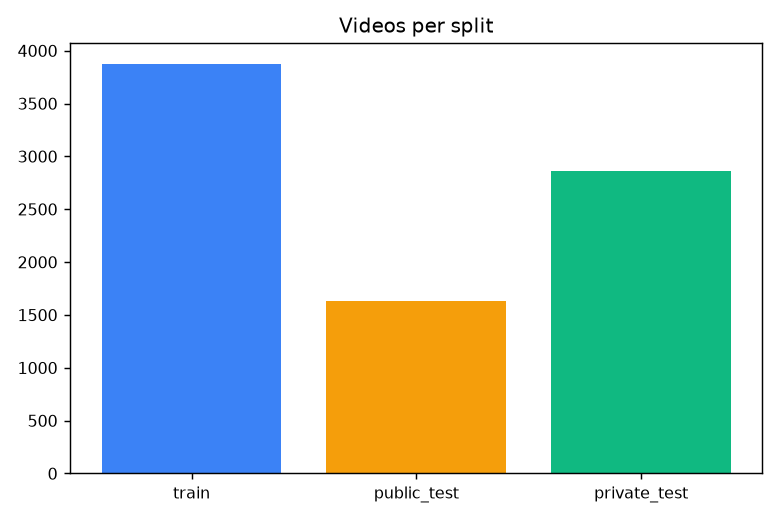
\includegraphics[width=0.6\textwidth]{split_sizes.png}
  \caption{Số lượng video trong ba tập \texttt{train}, \texttt{public\_test} và \texttt{private\_test}.}
  \label{fig:eda_split_sizes}
\end{figure}

\paragraph{Định dạng video} Toàn bộ 8.364 tệp đều là \texttt{.mp4} và đọc được; không có video nào có 0 khung hình. Độ phân giải đồng nhất tuyệt đối: 100\% video ở cả ba tập đều là $224\times224$ (Bảng~\ref{tab:eda_res}). Số khung hình gần như cố định ở mức 30 (chi tiết ở Mục~\ref{subsec:eda_uni}).

\begin{table}[H]
  \centering
  \caption{Thống kê độ phân giải video.}
  \label{tab:eda_res}
  \begin{tabular}{@{}lrrr@{}}
    \toprule
    \textbf{Tập} & \textbf{Độ phân giải} & \textbf{Số video} & \textbf{Tỷ lệ} \\
    \midrule
    train         & $224\times224$ & 3.875 & 100\% \\
    public\_test  & $224\times224$ & 1.630 & 100\% \\
    private\_test & $224\times224$ & 2.859 & 100\% \\
    \bottomrule
  \end{tabular}
\end{table}

\paragraph{Quan sát trực quan} Để kiểm chứng bằng mắt, nhóm trích 6--8 khung hình phân bố đều trong video (\texttt{cap.set(cv2.CAP\_\allowbreak PROP\_\allowbreak POS\_\allowbreak FRAMES, i)} với $i$ lấy từ \texttt{np.linspace}) và ghép thành lưới ảnh cho một số lớp (Hình~\ref{fig:eda_samples}). Các video được quay chính diện, người ký ngồi hoặc đứng giữa khung hình, thấy rõ phần thân trên, hai tay và khuôn mặt; nền chủ yếu là tường trơn với ánh sáng trong nhà. Sự đa dạng nằm ở người ký (giới tính, trang phục, kính), màu nền (be, xanh nhạt, trắng) và vị trí tay lúc bắt đầu. Ký hiệu thường chỉ chiếm một phần thời lượng: các khung đầu và cuối thường là tư thế nghỉ. Ở một số video xuất hiện các khung \emph{đơn sắc hoàn toàn} (hàng \textit{Phỏng vấn}, \textit{Uống}); hiện tượng này được định lượng ở Mục~\ref{subsec:eda_quality}.

\begin{figure}[H]
  \centering
  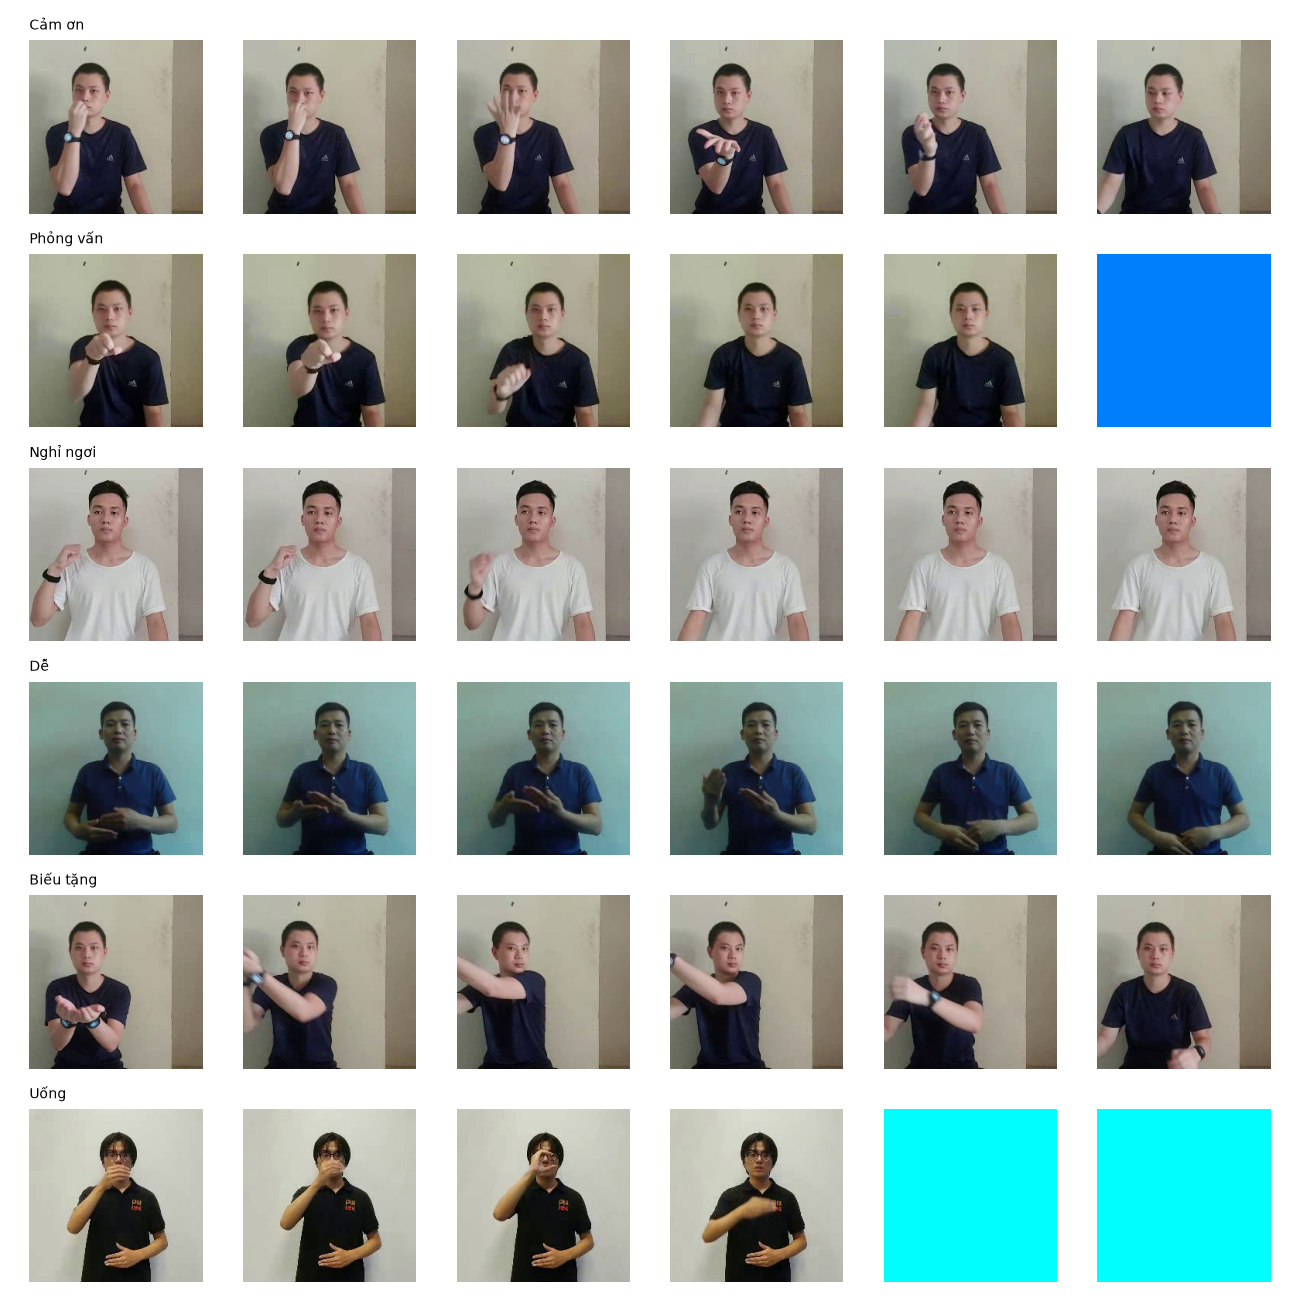
\includegraphics[width=0.85\textwidth]{sample_frames_6classes.png}
  \caption{Khung hình mẫu (lấy đều theo thời gian) của sáu lớp. Hàng \textit{Phỏng vấn} và \textit{Uống} có các khung đơn sắc ở cuối video.}
  \label{fig:eda_samples}
\end{figure}

\noindent\textit{Hệ quả:} khi gán nhãn số cho video phải chuẩn hoá tên lớp bằng \texttt{unicodedata.normalize(\textquotesingle NFC\textquotesingle, ...)} trước khi tra \texttt{label\_mapping.pkl}, nếu không phần lớn video sẽ không tìm được nhãn. Chỉ có tập \texttt{train} mang nhãn nên tập kiểm định (\textit{validation}) phải tách ra từ chính tập này; việc tách cần tính đến trùng lặp (Mục~\ref{subsec:eda_quality}). Thông tin phân biệt nằm ở hình dạng và chuyển động của bàn tay, khẩu hình và tư thế, nên các phép tăng cường không được làm đổi ngữ nghĩa không gian; đặc biệt \emph{không} dùng lật ngang (\textit{Horizontal Flip}) vì có thể đổi nghĩa tay trái/phải.

% =====================================================================
\subsubsection{Chất lượng dữ liệu}
\label{subsec:eda_quality}

\paragraph{Script và cách thực hiện}
\begin{itemize}
  \item \textbf{Script:} bốn script trong \texttt{02\_data\_quality/}, chạy theo thứ tự: \edafile{02\_data\_quality}{01\_integrity\_missing.py}, \edafile{02\_data\_quality}{02\_duplicates.py}, \edafile{02\_data\_quality}{03\_frame\_scan.py}, \edafile{02\_data\_quality}{04\_frame\_quality\_summary.py}. Kiểm tra bằng mắt dùng \edafile{07\_visual\_inspection}{02\_flagged\_videos.py}.
  \item \textbf{Cách khai thác dữ liệu:} 
  
  (i) \emph{Giá trị thiếu và lỗi đọc:} \texttt{01\_integrity\_missing.py} đếm ô trống (\texttt{isna}) theo cột và theo tập, đếm video có 0 khung, FPS hoặc kích thước bằng 0, rồi liệt kê các tệp có giá trị phi lý theo ngưỡng tuyệt đối (dưới 10~KB, dưới 16 khung, FPS dưới 5). 
  
  (ii) \emph{Trùng lặp:} \texttt{02\_duplicates.py} đọc toàn bộ byte của từng tệp, tính \texttt{hashlib.md5} một lần và lưu vào \texttt{file\_hashes.csv}; hai tệp cùng mã băm là cùng nội dung. Gom nhóm theo mã băm để đếm bản sao, tìm nhóm có nhiều hơn một nhãn (xung đột nhãn), lấy giao các tập mã băm giữa train, public test, private test, rồi giữ một tệp cho mỗi mã băm và đếm lại số video mỗi lớp. 
  
  (iii) \emph{Khung đơn sắc:} \texttt{03\_frame\_scan.py} giải mã \emph{từng} khung bằng \texttt{cap.read()}, tính độ lệch chuẩn điểm ảnh của từng kênh màu và coi khung là đơn sắc khi giá trị lớn nhất nhỏ hơn 3; đồng thời đếm số khung đơn sắc liên tiếp ở đầu video và tính độ chuyển động là trung bình $|f_t-f_{t-1}|$ trên ảnh xám. \texttt{04\_frame\_quality\_summary.py} đối chiếu số khung đọc được với metadata, bỏ các bản sao \texttt{\_N}, phân loại vị trí khung đơn sắc (đầu, cuối, giữa, toàn bộ) và mô phỏng việc lấy $T=16$ khung bằng \texttt{np.linspace} để đếm số khung đơn sắc bị lấy trúng. 
  
  (iv) \emph{Kiểm tra bằng mắt:} \texttt{02\_flagged\_videos.py} \emph{tự chọn} video cần xem từ kết quả hai bước trên, không dùng danh sách chọn tay. Tiêu chí chọn gồm: 6 video có tỷ lệ khung đơn sắc cao nhất trong số các video có từ 50\% khung đơn sắc trở lên; mọi video thuộc nhóm MD5 nằm ở hơn một lớp; một ví dụ cho mỗi dạng xuất hiện khung đơn sắc. Ngoại lai theo quy tắc Tukey được tính ở bước đơn biến (Mục~\ref{subsec:eda_uni}).
  \item \textbf{Đầu ra:} \texttt{integrity\_summary.txt}, \texttt{file\_hashes.csv}, \texttt{dups\_summary.txt}, \texttt{dedup\_summary.txt}, \texttt{class\_counts\_train\_unique\_vs\_all.csv}, \texttt{video\_quality\_flags.csv}, \texttt{solid\_frame\_summary.txt}, \texttt{class\_solid\_frame\_ratio.csv}; ở bước kiểm tra bằng mắt là \texttt{flagged\_videos\_info.txt}, \texttt{flagged\_videos\_check.png}, \texttt{solid\_frame\_patterns.png}.
\end{itemize}

Nhóm kiểm tra chất lượng dữ liệu theo các khía cạnh: giá trị thiếu, bản ghi trùng lặp, khung hình đơn sắc/video rỗng, giá trị ngoại lai, nhiễu nhãn và trùng lặp giữa các tập. Bảng~\ref{tab:eda_quality} tóm tắt các vấn đề phát hiện được.

\begin{table}[H]
  \centering
  \caption{Tóm tắt các vấn đề chất lượng dữ liệu.}
  \label{tab:eda_quality}
  \small
  \begin{tabular}{@{}p{0.26\textwidth}p{0.36\textwidth}p{0.30\textwidth}@{}}
    \toprule
    \textbf{Vấn đề} & \textbf{Số lượng} & \textbf{Ví dụ} \\
    \midrule
    Bản sao hậu tố \texttt{\_N} trong train & 1.069 tệp giống hệt bản gốc; còn 2.776 video duy nhất & \texttt{127824.mp4}, \texttt{127824\_1.mp4}, \texttt{127824\_2.mp4} \\
    Video có khung đơn sắc (train) & 758/3.875 tệp; 565/2.776 video duy nhất (20,4\%), ở 78/100 lớp & \texttt{Thất lạc/708519}, \texttt{Bộ y tế/523389} \\
    Video rỗng hoàn toàn & 2 video gốc (4 tệp kể cả bản sao) & \texttt{Biết/214576}, \texttt{Khai báo/885339} \\
    Nhiễu nhãn (cùng nội dung, khác lớp) & 2 nhóm nội dung, 5 tệp & \textit{Chậm lại} $\leftrightarrow$ \textit{Chào} \\
    Trùng train $\rightarrow$ public test & 157 video public giống hệt video train & -- \\
    Trùng public $\leftrightarrow$ private & 896 video & -- \\
    \bottomrule
  \end{tabular}
\end{table}

\paragraph{Giá trị thiếu và lỗi đọc} Bảng metadata không có giá trị thiếu ở bất kỳ thuộc tính nào (nhãn \texttt{cls} chỉ trống ở hai tập test vì các tập này vốn không có nhãn). Mọi video đều mở và giải mã được, và ở cả 8.364 video, số khung giải mã thực tế khớp với số khung ghi trong metadata. Như vậy không có vấn đề về tệp hỏng hay nhãn bị thiếu ở tập train.

\paragraph{Trùng lặp trong tập train} Nhóm tính mã băm MD5 nội dung từng tệp (\texttt{hashlib.md5}) rồi gom nhóm theo mã băm. Có 1.069/3.875 tệp mang hậu tố \texttt{\_1}, \texttt{\_2}, \texttt{\_3}\ldots{} So sánh từng cặp cho thấy cả 1.069 tệp này đều có bản gốc tồn tại, cùng lớp và \emph{giống hệt bản gốc từng byte} (cùng số khung, FPS, dung lượng): đây là bản sao, không phải biến thể tăng cường. Có 176 video gốc có 1 bản sao, 169 video có 2 và 185 video có 3. Tính cả các bản sao khác, tập train có 1.099 tệp dư thừa và chỉ còn \textbf{2.776 video duy nhất}. Các bản sao tập trung ở những lớp vốn đã nhiều mẫu (\textit{Chậm lại} và \textit{Trường học} cùng thêm 25 tệp, \textit{Rau} và \textit{Nhìn} thêm 23, \textit{Khóc} thêm 22\ldots), nên sau khi khử trùng lặp số video mỗi lớp còn từ 5 đến 51 (trung bình 27,8; tỷ lệ chênh $\approx$10,2 lần). Bảng trước/sau khử trùng lặp của từng lớp lưu ở \texttt{class\_counts\_train\_unique\_vs\_all.csv}. Hệ quả là nguy cơ rò rỉ dữ liệu (\textit{Data Leakage}): nếu chia train/validation ngẫu nhiên theo từng tệp, các bản sao của cùng một video rơi vào cả hai phần, làm điểm validation bị thổi phồng.

\paragraph{Khung hình đơn sắc và video rỗng} Nhóm đọc \emph{toàn bộ} khung hình của 8.364 video và tính độ lệch chuẩn giá trị điểm ảnh trên từng kênh màu; khung có độ lệch chuẩn lớn nhất giữa ba kênh nhỏ hơn 3 được coi là \emph{khung đơn sắc}. Kết quả tổng hợp ở Bảng~\ref{tab:eda_solid}.

\begin{table}[H]
  \centering
  \caption{Số video chứa khung hình đơn sắc theo từng tập.}
  \label{tab:eda_solid}
  \begin{tabular}{@{}lrrrr@{}}
    \toprule
    \textbf{Tập} & \textbf{Tổng video} & \textbf{Có $\geq$1 khung đơn sắc} & \textbf{Đơn sắc toàn bộ} & \textbf{Tỷ lệ} \\
    \midrule
    train (tất cả tệp)        & 3.875 & 758 & 4 & 19,6\% \\
    train (video duy nhất)    & 2.776 & 565 & 2 & 20,4\% \\
    public\_test              & 1.630 & 1   & 0 & 0,06\% \\
    private\_test             & 2.859 & 1   & 0 & 0,03\% \\
    \bottomrule
  \end{tabular}
\end{table}

Đây là phát hiện đáng chú ý nhất của EDA. Khoảng một phần năm số video duy nhất trong train (565/2.776, thuộc 78/100 lớp) chứa khung đơn sắc, và số khung này không nhỏ: trung bình 12,2 khung trên khoảng 30 khung mỗi video (trung vị 12, nhiều nhất 23). Các khung có màu thuần (đỏ, xanh lục, xanh lam, xanh lục lam, tím, vàng, trắng, đen, xám) và xuất hiện theo các dạng: chỉ ở đầu video (231 video), chỉ ở cuối (161), cả đầu và cuối (116), xen ở giữa (55) hoặc toàn bộ video (2) (Hình~\ref{fig:eda_solid_examples}). Lớp có tỷ lệ video bị ảnh hưởng cao nhất là \textit{Có thể} (6/15 video duy nhất), \textit{Xin lỗi} (5/14) và \textit{Thất lạc} (7/20) (chi tiết ở \texttt{class\_solid\_frame\_ratio.csv}).

\begin{figure}[H]
  \centering
  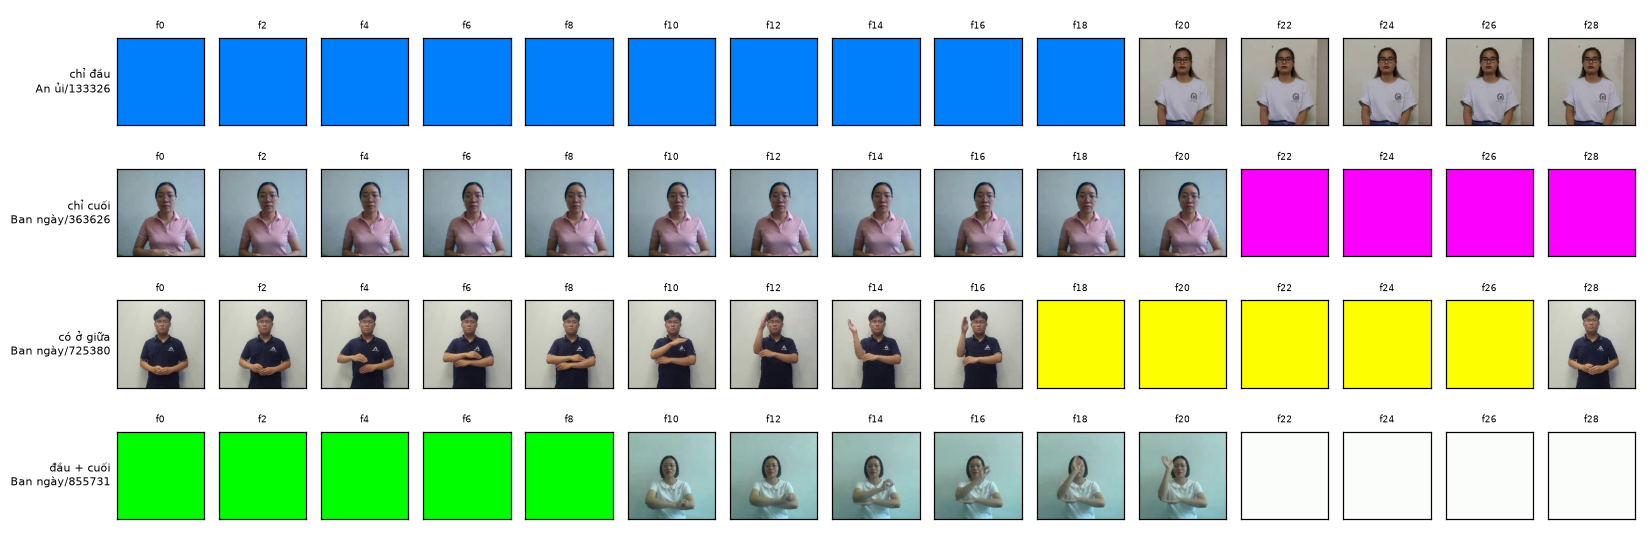
\includegraphics[width=\textwidth]{solid_frame_patterns.png}
  \caption{Bốn dạng khung đơn sắc trong tập train (khung chẵn $f_0$--$f_{28}$), mỗi dạng một video được chọn tự động: chỉ ở đầu (\textit{An ủi}/133326), chỉ ở cuối (\textit{Ban ngày}/363626), xen ở giữa (\textit{Ban ngày}/725380), cả đầu và cuối (\textit{Ban ngày}/855731).}
  \label{fig:eda_solid_examples}
\end{figure}

Hiện tượng này ảnh hưởng trực tiếp đến cách lấy mẫu: khi lấy $T=16$ khung đều nhau bằng \texttt{linspace} trên 565 video nói trên, trung bình có 6,4/16 khung được chọn là khung đơn sắc, và ở 224 video có từ 8/16 khung trở lên (ít nhất một nửa chuỗi đầu vào) là khung đơn sắc. Ngược lại, mỗi tập test chỉ có 1 video chứa đúng 1 khung đơn sắc. Như vậy khung đơn sắc là đặc điểm \emph{riêng của tập train}: nếu không xử lý, mô hình vừa mất thông tin ký hiệu, vừa có thể học các tín hiệu giả không tồn tại ở dữ liệu kiểm tra.

Sáu hàng đầu của Hình~\ref{fig:eda_suspicious} là các video có tỷ lệ khung đơn sắc cao nhất. Hai video được xác nhận bằng mắt là \textbf{rỗng hoàn toàn}: \texttt{Biết/214576.mp4} (2,5~KB, 16 khung, toàn màu xanh lục) và \texttt{Khai báo/885339.mp4} (2,7~KB, 23 khung, toàn màu xanh lam, kèm 2 bản sao \texttt{\_1}, \texttt{\_2}); cả hai không có người ký. Bốn video tiếp theo có 20--21/30 khung đơn sắc: \texttt{Nôn ói/915809}, \texttt{Thất lạc/708519}, \texttt{Chân/984642} và \texttt{Khai báo/362529}. Người ký chỉ xuất hiện trong khoảng 10 khung, ví dụ \texttt{Khai báo/362529} có 20 khung đỏ đầu tiên ($f_0$--$f_{19}$).

\paragraph{Giá trị ngoại lai} Nhóm dùng quy tắc Tukey (ngoài khoảng $[Q_1-1{,}5\,\mathrm{IQR},\,Q_3+1{,}5\,\mathrm{IQR}]$ tính trên tập train) cho thời lượng, dung lượng và FPS. Số lượng ngoại lai khá nhiều nhưng phần lớn chỉ lệch nhẹ (Mục~\ref{subsec:eda_uni}). Đáng chú ý là các ngoại lai cực đoan: thời lượng trên 5~s có 10 video train, 1 video public test và 3 video private test (lớn nhất 35,3~s ở train, 28,1~s ở private test); FPS dưới 5 có 9 video train và 2 video private test; dung lượng dưới 10~KB có 4 tệp train, đều là các video rỗng nói trên. Các ngoại lai này không nhất thiết là lỗi mà phản ánh việc video được lấy mẫu lại về $\approx$30 khung từ các clip gốc có độ dài rất khác nhau.

\paragraph{Nhiễu nhãn} Khi gom nhóm theo MD5, có hai nhóm nội dung giống hệt nhau nhưng nằm ở \emph{hai lớp khác nhau}: \texttt{Chậm lại/284430.mp4} trùng với \texttt{Chào/392683.mp4} và \texttt{Chào/468203.mp4}; \texttt{Chậm lại/254739.mp4} trùng với \texttt{Chào/792094.mp4}. Nhóm đã xem trực tiếp (Hình~\ref{fig:eda_suspicious}, năm hàng cuối) và xác nhận chúng có cùng người ký, cùng chuỗi động tác. Một video không thể đồng thời mang hai nghĩa nên ít nhất một trong hai nhãn là sai; tuy nhiên việc xác định nhãn đúng cần người am hiểu ngôn ngữ ký hiệu Việt Nam, nên báo cáo chỉ ghi nhận đây là \emph{xung đột nhãn}.

\begin{figure}[H]
  \centering
  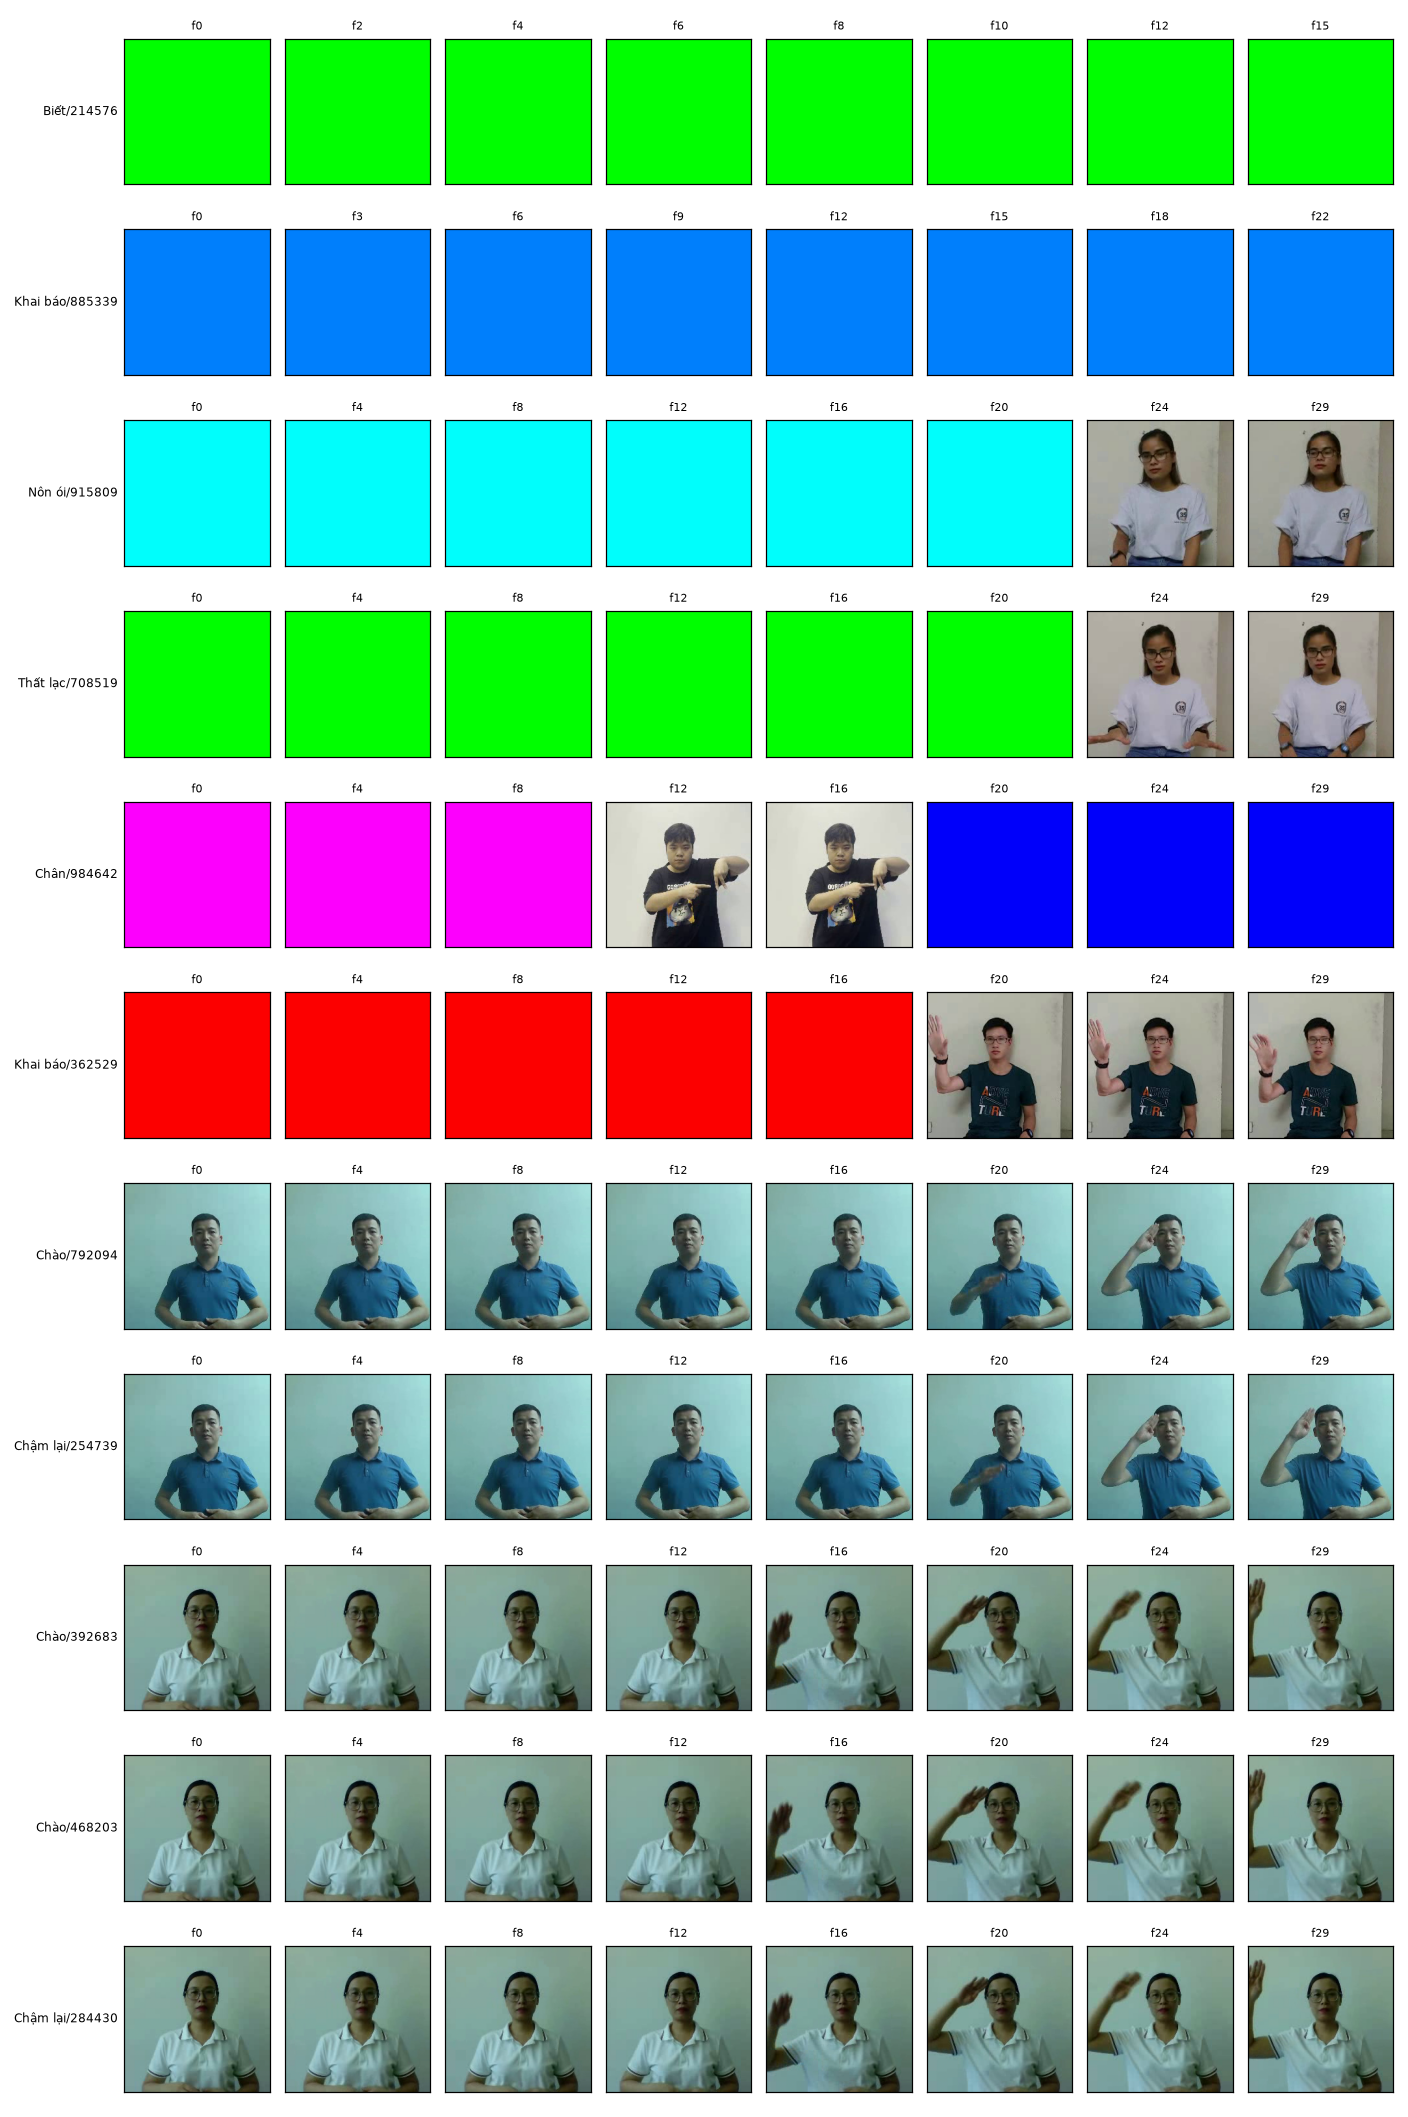
\includegraphics[width=0.9\textwidth,height=0.72\textheight,keepaspectratio]{flagged_videos_check.png}
  \caption{Kiểm tra bằng mắt các video do bước kiểm tra chất lượng tự đánh dấu. Sáu hàng đầu là các video có tỷ lệ khung đơn sắc cao nhất, gồm hai video rỗng hoàn toàn (\textit{Biết}/214576, \textit{Khai báo}/885339). Năm hàng cuối là hai nhóm video trùng nội dung nhưng khác nhãn (\textit{Chậm lại} $\leftrightarrow$ \textit{Chào}).}
  \label{fig:eda_suspicious}
\end{figure}

\paragraph{Trùng lặp giữa các tập} Public test có 8 bản trùng nội bộ (1.622 video duy nhất) và \textbf{157 video giống hệt video trong train}; private test có 2.782 video duy nhất, không trùng với train, nhưng có 896 video trùng với public test. Ngoài ra, 2.806 tên tệp trong private test trùng với tên tệp trong train nhưng nội dung hoàn toàn khác (MD5 khác, chênh lệch điểm ảnh lớn), nên đây chỉ là trùng cách đặt mã số; nguyên nhân chưa rõ và tên tệp \emph{không} được dùng để suy luận nhãn.

\noindent\textit{Hệ quả:} dữ liệu train chưa sạch; trước khi huấn luyện cần khử trùng lặp, loại video rỗng, xử lý khung đơn sắc và rà soát các nhãn xung đột. Điểm trên public test có thể bị ảnh hưởng một phần bởi 157 video đã có trong train.

% =====================================================================
\subsubsection{Phân tích đơn biến}
\label{subsec:eda_uni}

\paragraph{Script và cách thực hiện}
\begin{itemize}
  \item \textbf{Script:} \edafile{03\_univariate}{01\_numeric\_attributes.py}.
  \item \textbf{Cách khai thác dữ liệu:} với mỗi thuộc tính số (\texttt{frames}, \texttt{fps}, \texttt{dur}, \texttt{size\_kb}), script tính \texttt{groupby(\textquotesingle split\textquotesingle).describe()} (trung bình, độ lệch chuẩn, min, các tứ phân vị, max), hệ số lệch (\textit{skewness}) và các giá trị phổ biến nhất. Ngoại lai được xác định theo quy tắc Tukey với ngưỡng tính trên train rồi áp lên cả ba tập. Script vẽ histogram của từng thuộc tính cho ba tập trên cùng trục; histogram FPS và dung lượng dùng mật độ (\texttt{density=True}) để so sánh được các tập có kích thước khác nhau.
  \item \textbf{Đầu ra:} \texttt{desc\_by\_split.csv} (Bảng~\ref{tab:eda_desc}), \texttt{univariate\_summary.txt}, \texttt{frames\_hist\_by\_split.png}, \texttt{fps\_hist\_by\_split.png}, \texttt{filesize\_hist\_by\_split.png}.
\end{itemize}

Mục này khảo sát phân phối của từng thuộc tính số: số khung hình, FPS, thời lượng và dung lượng, tính trên từng tập (Bảng~\ref{tab:eda_desc}). Độ phân giải đã được trình bày ở Bảng~\ref{tab:eda_res}.

\begin{table}[H]
  \centering
  \caption{Thống kê mô tả các thuộc tính số theo từng tập.}
  \label{tab:eda_desc}
  \small
  \begin{tabular}{@{}llrrrrrrr@{}}
    \toprule
    \textbf{Thuộc tính} & \textbf{Tập} & \textbf{Mean} & \textbf{Std} & \textbf{Min} & \textbf{Q1} & \textbf{Median} & \textbf{Q3} & \textbf{Max} \\
    \midrule
    \multirow{3}{*}{Số khung}
      & train   & 29,88 & 1,26 & 16 & 30 & 30 & 30 & 30 \\
      & public  & 29,96 & 0,66 & 16 & 30 & 30 & 30 & 30 \\
      & private & 29,98 & 0,44 & 21 & 30 & 30 & 30 & 30 \\
    \midrule
    \multirow{3}{*}{FPS}
      & train   & 12,94 & 3,11 & 0,85 & 10,98 & 12,34 & 14,06 & 30,02 \\
      & public  & 12,97 & 3,00 & 5,93 & 10,98 & 12,50 & 13,85 & 30,00 \\
      & private & 13,32 & 3,69 & 1,07 & 10,84 & 12,50 & 14,06 & 30,02 \\
    \midrule
    \multirow{3}{*}{Thời lượng (s)}
      & train   & 2,48 & 1,36 & 0,70 & 2,13 & 2,43 & 2,73 & 35,29 \\
      & public  & 2,42 & 0,51 & 0,70 & 2,17 & 2,40 & 2,73 & 5,06 \\
      & private & 2,42 & 0,82 & 0,70 & 2,13 & 2,40 & 2,77 & 28,14 \\
    \midrule
    \multirow{3}{*}{Dung lượng (KB)}
      & train   & 85,5  & 38,5 & 2,5  & 60,2 & 80,6 & 103,0 & 263,8 \\
      & public  & 113,6 & 77,5 & 26,2 & 76,1 & 91,0 & 125,8 & 483,2 \\
      & private & 116,3 & 77,7 & 42,2 & 77,7 & 94,6 & 126,0 & 488,0 \\
    \bottomrule
  \end{tabular}
\end{table}

\paragraph{Số khung hình} Hầu hết video có đúng 30 khung: 3.832/3.875 video train (98,9\%), 1.623/1.630 public test và 2.850/2.859 private test; ở train có 26 video chỉ có 16 khung. Không video nào ngắn hơn 16 khung (Hình~\ref{fig:eda_frames_hist}), nên không cần đệm khung thực sự khi lấy $T=16$.

\begin{figure}[H]
  \centering
  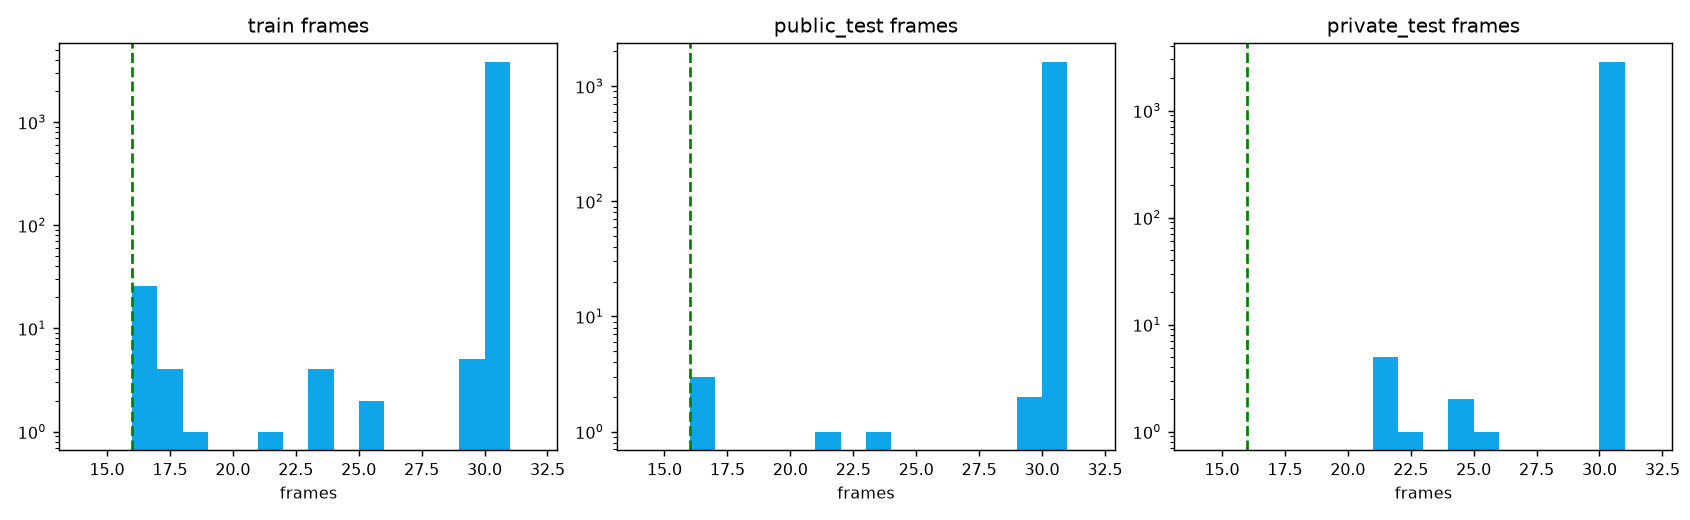
\includegraphics[width=\textwidth]{frames_hist_by_split.png}
  \caption{Histogram số khung hình mỗi video theo tập (trục tung thang log). Đường đứt nét đánh dấu $T=16$.}
  \label{fig:eda_frames_hist}
\end{figure}

\paragraph{FPS và thời lượng} Dù số khung gần như cố định, FPS biến thiên mạnh: train có 961 giá trị FPS khác nhau, từ 0,85 đến 30,02 (trung vị 12,3), phân phối lệch phải với đuôi dài (hệ số lệch 1,01 ở train; Hình~\ref{fig:eda_fps_hist}). Vì thời lượng $=\texttt{frames}/\texttt{fps}$ nên thời lượng thực của cùng 30 khung dao động lớn: trung vị khoảng 2,4~s nhưng có video tới 35,3~s ở train và 28,1~s ở private test, trong khi 99\% video đều ngắn hơn khoảng 4~s. Điều này cho thấy video đã được lấy mẫu lại về khoảng 30 khung bất kể độ dài clip gốc.

\begin{figure}[H]
  \centering
  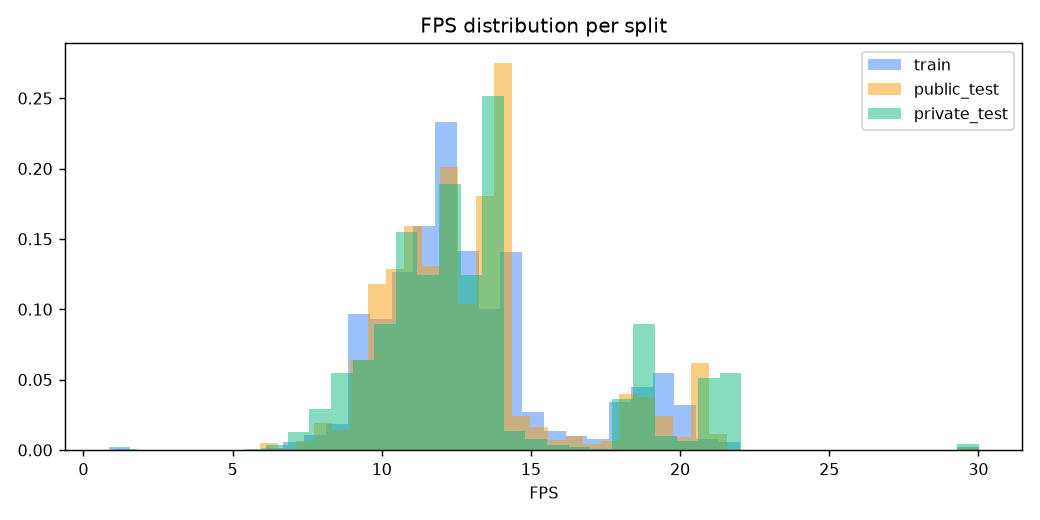
\includegraphics[width=0.85\textwidth]{fps_hist_by_split.png}
  \caption{Phân phối FPS theo từng tập.}
  \label{fig:eda_fps_hist}
\end{figure}

\paragraph{Dung lượng tệp} Dung lượng train có trung vị 80,6~KB (trung bình 85,5; từ 2,5 đến 263,8~KB). Hai tập test có phân phối lệch phải hơn hẳn: trung bình 113,6--116,3~KB, lớn nhất tới 483--488~KB (Hình~\ref{fig:eda_size_hist}); khác biệt này được phân tích ở Mục~\ref{subsec:eda_shift}.

\begin{figure}[H]
  \centering
  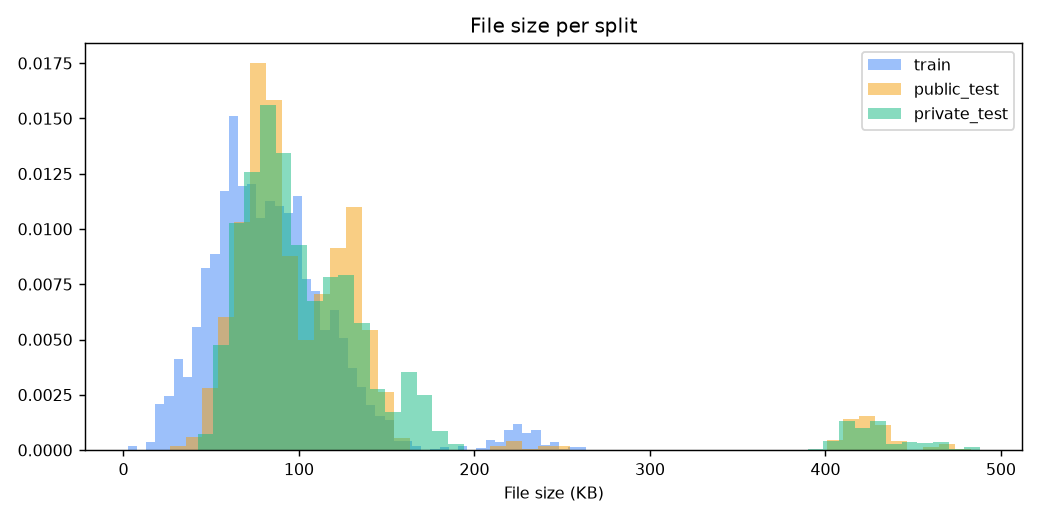
\includegraphics[width=0.85\textwidth]{filesize_hist_by_split.png}
  \caption{Phân phối dung lượng tệp (KB) theo từng tập.}
  \label{fig:eda_size_hist}
\end{figure}

\noindent\textit{Hệ quả:} (i) không cần đổi kích thước khung hình, tuy kiến trúc CRNN với \texttt{Adaptive\allowbreak AvgPool2d} vẫn đảm bảo tính tổng quát nếu gặp video khác độ phân giải; (ii) vì mọi video có ít nhất 16 khung, lấy mẫu $T=16$ khung đều nhau bằng \texttt{linspace} (\textit{Frame Downsampling}) là đủ, lặp khung (\textit{repeat padding}) chỉ giữ làm phương án dự phòng; (iii) phân phối FPS và dung lượng lệch phải với nhiều ngoại lai nên nên dùng trung vị thay vì trung bình khi mô tả.

% =====================================================================
\subsubsection{Phân tích biến mục tiêu}
\label{subsec:eda_class}

\paragraph{Script và cách thực hiện}
\begin{itemize}
  \item \textbf{Script:} \edafile{04\_target\_analysis}{01\_class\_distribution.py}.
  \item \textbf{Cách khai thác dữ liệu:} lọc các dòng của tập train trong \texttt{video\_metadata.csv}, đếm số video mỗi nhãn bằng \texttt{value\_counts()}, sau đó tính trung bình, trung vị, độ lệch chuẩn, tỷ lệ lớp lớn nhất/nhỏ nhất và số lớp có không quá 25 hoặc từ 50 video trở lên. Số video mỗi lớp sau khử trùng lặp lấy từ \texttt{class\_counts\_train\_unique\_vs\_all.csv} của bước \texttt{02\_data\_quality}.
  \item \textbf{Đầu ra:} \texttt{class\_summary.txt}, \texttt{class\_counts\_train.csv}, \texttt{class\_distribution\_all.png}, \texttt{class\_top\_bottom10.png}, \texttt{samples\_per\_class\_hist.png}.
\end{itemize}

Nhóm dùng \texttt{value\_counts()} trên cột nhãn của tập \texttt{train} để đếm số video mỗi lớp, rồi vẽ biểu đồ cho cả 100 lớp (Hình~\ref{fig:eda_class_dist}), 10 lớp nhiều nhất/ít nhất (Hình~\ref{fig:eda_top_bottom}) và histogram số video mỗi lớp (Hình~\ref{fig:eda_spc_hist}).

\begin{figure}[H]
  \centering
  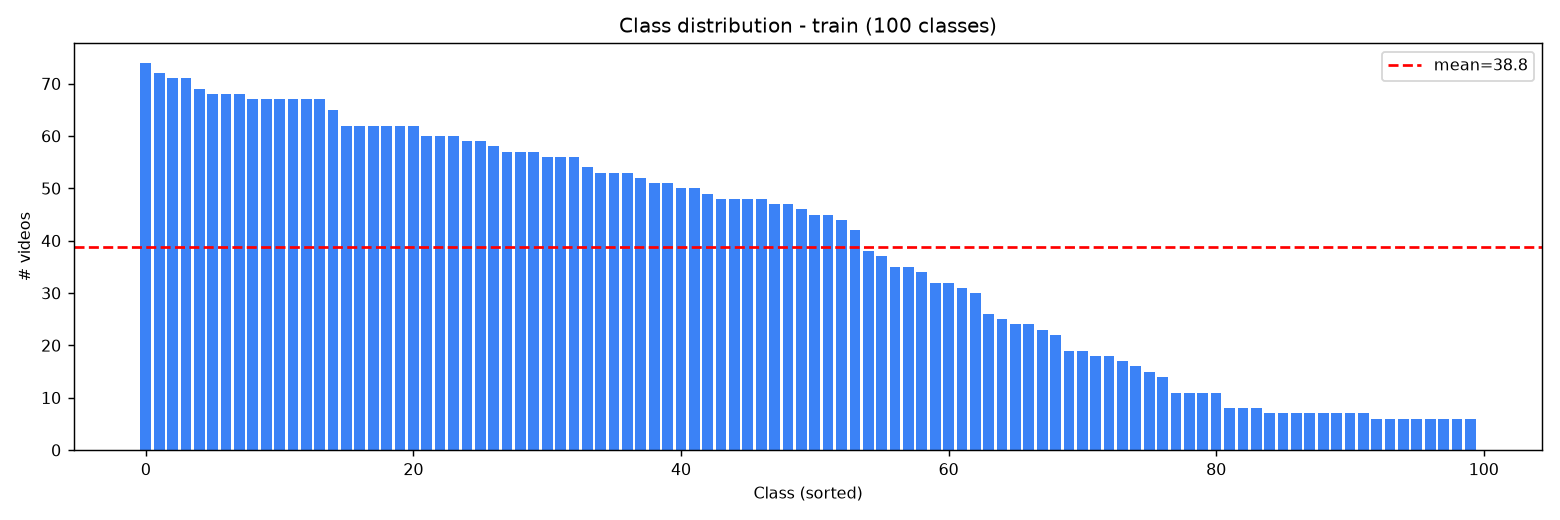
\includegraphics[width=\textwidth]{class_distribution_all.png}
  \caption{Phân phối số video theo lớp trong tập huấn luyện (100 lớp, sắp xếp giảm dần).}
  \label{fig:eda_class_dist}
\end{figure}

Tập huấn luyện gồm 3.875 video nhưng phân bố không đồng đều: trung bình 38,75 video/lớp, trung vị 45,5, độ lệch chuẩn 22,78. Lớp nhiều nhất (\textit{Trường học}) có 74 video, trong khi mười lớp chỉ có 6--7 video; tỷ lệ chênh giữa lớp lớn nhất và nhỏ nhất xấp xỉ $12{,}3$ lần (Bảng~\ref{tab:eda_top_bottom}). Có 36/100 lớp có không quá 25 video và 42/100 lớp có từ 50 video trở lên, tức phân phối có dạng hai đỉnh: nhóm lớp ``giàu'' (khoảng 45--74 video) và nhóm lớp ``nghèo'' (khoảng 6--11 video). Nhiều lớp ít mẫu thuộc nhóm từ vựng y tế -- dịch bệnh.

\begin{table}[H]
  \centering
  \caption{Mười lớp nhiều mẫu nhất và mười lớp ít mẫu nhất trong tập huấn luyện.}
  \label{tab:eda_top_bottom}
  \begin{tabular}{@{}lr@{\hspace{2.5em}}lr@{}}
    \toprule
    \multicolumn{2}{c}{\textbf{Nhiều nhất}} & \multicolumn{2}{c}{\textbf{Ít nhất}} \\
    \cmidrule(r){1-2}\cmidrule(l){3-4}
    \textbf{Lớp} & \textbf{Số video} & \textbf{Lớp} & \textbf{Số video} \\
    \midrule
    Trường học & 74 & Nhầm      & 7 \\
    Rau        & 72 & Virus     & 7 \\
    Nhà        & 71 & Bệnh nhân & 6 \\
    Áp dụng    & 71 & Cách ly   & 6 \\
    Chậm lại   & 69 & Cơ thể    & 6 \\
    Cám dỗ     & 68 & Ho        & 6 \\
    Nghe       & 68 & Phục hồi  & 6 \\
    Nói xấu    & 68 & Sốt       & 6 \\
    Biết       & 67 & Xe máy    & 6 \\
    Chạy       & 67 & Ủng hộ    & 6 \\
    \bottomrule
  \end{tabular}
\end{table}

\begin{figure}[H]
  \centering
  \begin{minipage}{0.56\textwidth}
    \centering
    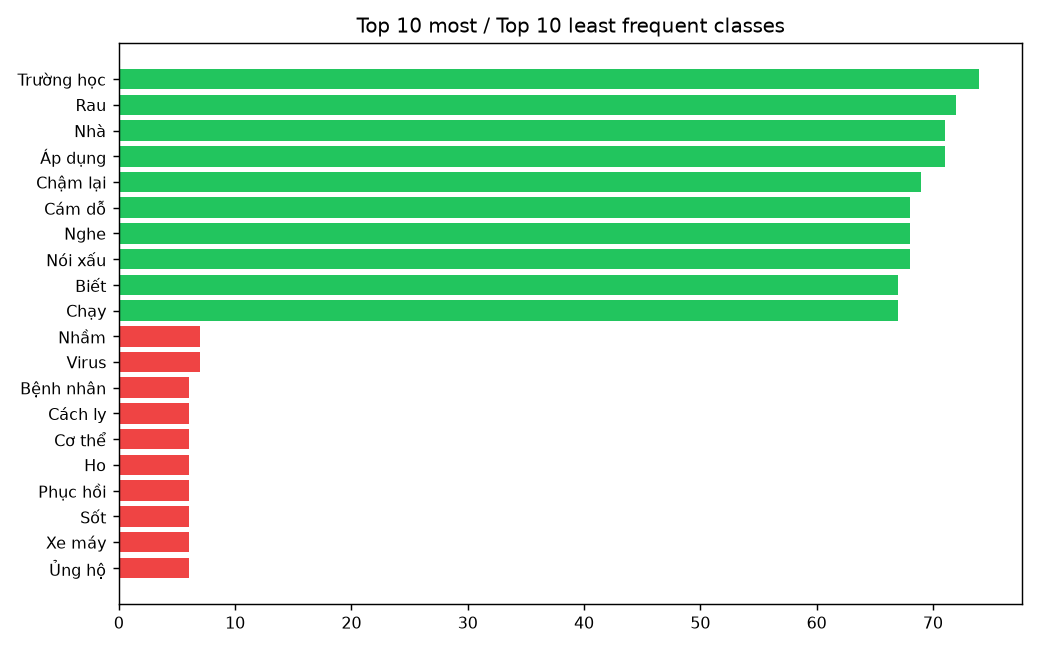
\includegraphics[width=\textwidth]{class_top_bottom10.png}
    \caption{Mười lớp nhiều nhất (xanh) và ít nhất (đỏ).}
    \label{fig:eda_top_bottom}
  \end{minipage}\hfill
  \begin{minipage}{0.42\textwidth}
    \centering
    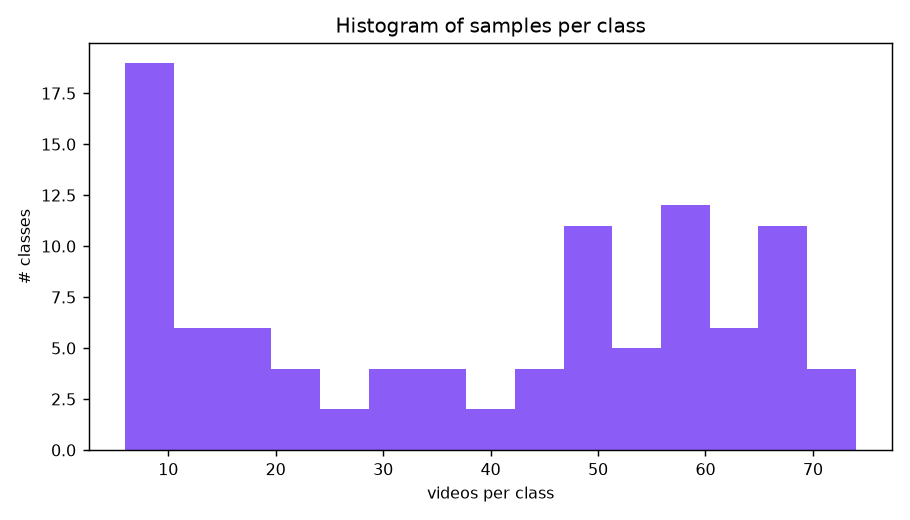
\includegraphics[width=\textwidth]{samples_per_class_hist.png}
    \caption{Histogram số video mỗi lớp.}
    \label{fig:eda_spc_hist}
  \end{minipage}
\end{figure}

Các con số trên tính trên tệp gốc, \emph{chưa} khử trùng lặp.

\noindent\textit{Hệ quả:} dữ liệu bị mất cân bằng lớp (\textit{Class Imbalance}) rõ rệt. Nếu đánh giá bằng Accuracy, mô hình có thể thiên về lớp phổ biến mà vẫn đạt điểm cao; vì vậy dùng Macro F1 (cũng là thước đo chính thức) và cần biện pháp xử lý mất cân bằng ở bước tiền xử lý/huấn luyện.

% =====================================================================
\subsubsection{Phân tích hai biến và đa biến}
\label{subsec:eda_multi}

\paragraph{Script và cách thực hiện}
\begin{itemize}
  \item \textbf{Script:} \edafile{05\_bivariate\_multivariate}{01\_correlation\_and\_label\_association.py}.
  \item \textbf{Cách khai thác dữ liệu:} ghép \texttt{video\_metadata.csv} với \texttt{video\_quality\_flags.csv} theo khoá (tập, lớp, tên tệp); bỏ các bản sao \texttt{\_N} để chỉ giữ 2.776 video duy nhất của train. Tính ma trận tương quan Pearson và Spearman (tương quan hạng, ít nhạy với ngoại lai) giữa các thuộc tính số; với từng thuộc tính, chia giá trị theo 100 lớp rồi chạy kiểm định Kruskal--Wallis (\texttt{scipy.stats.kruskal}) và tính $\eta^2 = SS_{\text{giữa lớp}}/SS_{\text{tổng}}$. Trung vị và tứ phân vị FPS của từng lớp được sắp xếp tăng dần để vẽ.
  \item \textbf{Đầu ra:} \texttt{multivariate\_summary.txt}, \texttt{corr\_heatmap.png}, \texttt{fps\_by\_class.png}, \texttt{size\_vs\_solid.png}.
\end{itemize}

Vì dữ liệu video không có đặc trưng dạng bảng, phân tích hai biến và đa biến tập trung vào mối quan hệ giữa các thuộc tính metadata với nhau và với nhãn lớp. Để tránh bản sao làm lệch kết quả, các phép tính dưới đây dùng 2.776 video duy nhất của tập train.

\paragraph{Tương quan giữa các thuộc tính} Hình~\ref{fig:eda_corr} cho thấy hệ số tương quan Pearson giữa số khung, FPS, dung lượng, tỷ lệ khung đơn sắc và độ chuyển động. (Thời lượng không đưa vào vì $\texttt{dur}=\texttt{frames}/\texttt{fps}$ nên phụ thuộc hoàn toàn vào hai biến còn lại.) Hầu hết các cặp có tương quan yếu ($|r|<0{,}35$); hai quan hệ rõ nhất là dung lượng -- tỷ lệ khung đơn sắc ($r\approx-0{,}45$; Spearman $\rho\approx-0{,}51$) và FPS -- chuyển động ($r\approx-0{,}34$; $\rho\approx-0{,}30$). Tương quan Spearman cho cùng chiều và độ lớn tương tự, nên các quan hệ này không phải do ngoại lai tạo ra. Quan hệ đầu là hợp lý: khung đơn sắc nén rất nhỏ nên video chứa nhiều khung đơn sắc có dung lượng thấp (Hình~\ref{fig:eda_size_solid}). Quan hệ sau cho thấy video có FPS thấp (clip gốc dài hơn) có độ chuyển động giữa các khung liên tiếp lớn hơn. Số khung gần như không liên quan tới các biến khác vì hầu như không đổi.

\begin{figure}[H]
  \centering
  \begin{minipage}{0.48\textwidth}
    \centering
    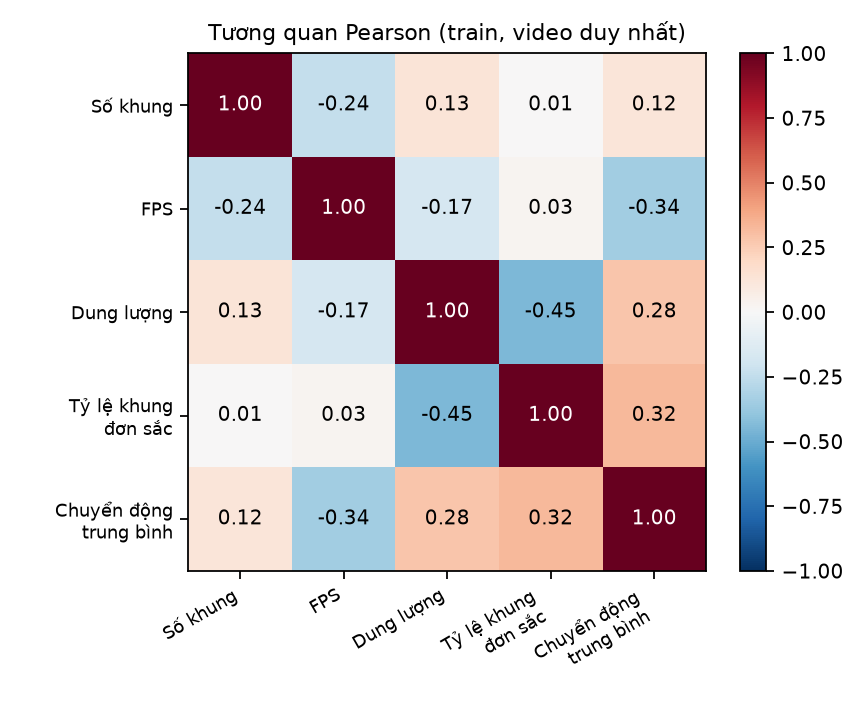
\includegraphics[width=\textwidth]{corr_heatmap.png}
    \caption{Ma trận tương quan Pearson giữa các thuộc tính (train, video duy nhất).}
    \label{fig:eda_corr}
  \end{minipage}\hfill
  \begin{minipage}{0.48\textwidth}
    \centering
    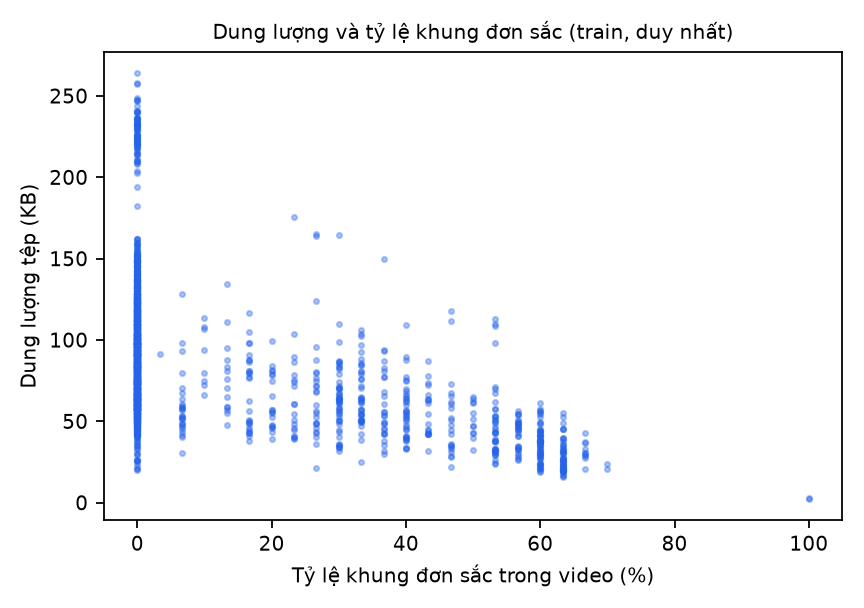
\includegraphics[width=\textwidth]{size_vs_solid.png}
    \caption{Dung lượng tệp theo tỷ lệ khung đơn sắc.}
    \label{fig:eda_size_solid}
  \end{minipage}
\end{figure}

\paragraph{Quan hệ giữa thuộc tính và nhãn lớp} Nhóm so sánh phân phối của từng thuộc tính giữa 100 lớp bằng kiểm định Kruskal--Wallis và hệ số $\eta^2$ (tỷ lệ phương sai giải thích bởi nhãn). Kết quả: FPS có $\eta^2\approx0{,}28$, dung lượng $\eta^2\approx0{,}15$, số khung $\eta^2\approx0{,}08$; cả ba đều có $p<10^{-10}$. Nói cách khác, FPS của video khác nhau rõ rệt giữa các lớp: trung vị FPS của lớp dao động từ khoảng 9,4 (\textit{Ngón tay}) đến khoảng 19,2 (\textit{Ho}), trong khi trung vị toàn tập là 12,4 (Hình~\ref{fig:eda_fps_class}). Điều này gợi ý rằng thời lượng clip gốc (và do đó FPS sau khi lấy mẫu lại) có liên hệ với từ được ký -- có thể vì các từ khác nhau có độ dài tự nhiên khác nhau -- hoặc vì cách thu thập dữ liệu theo từng lớp. Nhóm chưa xác định được nguyên nhân.

\begin{figure}[H]
  \centering
  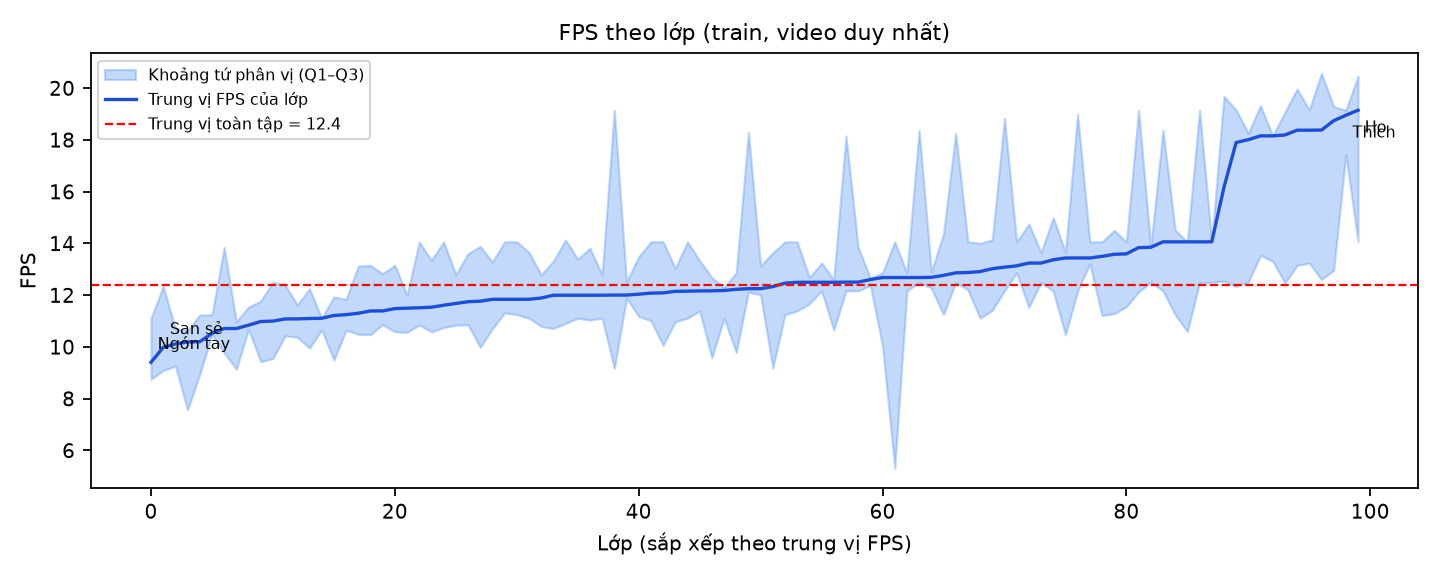
\includegraphics[width=0.95\textwidth]{fps_by_class.png}
  \caption{Trung vị và khoảng tứ phân vị của FPS theo lớp (train, video duy nhất), các lớp sắp xếp theo trung vị.}
  \label{fig:eda_fps_class}
\end{figure}

\paragraph{Khung đơn sắc theo lớp} Khung đơn sắc không phân bố đều: 78/100 lớp có ít nhất một video bị ảnh hưởng, và có lớp có tới 30--40\% video duy nhất chứa khung đơn sắc (\textit{Có thể}, \textit{Xin lỗi}, \textit{Thất lạc}, \textit{Mua}). Do đó việc loại bỏ khung đơn sắc sẽ tác động không đồng đều lên các lớp.

\noindent\textit{Hệ quả:} (i) các thuộc tính metadata phần lớn độc lập nhau nên không có cặp đặc trưng dư thừa cần loại bỏ; (ii) vì FPS và dung lượng có quan hệ thống kê với nhãn, chúng có thể trở thành ``đường tắt'' (\textit{shortcut}) mà mô hình học được thay vì học ký hiệu, nên không nên đưa FPS hoặc dung lượng làm đặc trưng đầu vào và cần theo dõi nguy cơ này khi đánh giá; (iii) cần kiểm tra lại phân phối nhãn sau khi loại khung đơn sắc.

% =====================================================================
\subsubsection{So sánh phân phối giữa các tập}
\label{subsec:eda_shift}

\paragraph{Script và cách thực hiện}
\begin{itemize}
  \item \textbf{Script:} \edafile{06\_split\_comparison}{01\_split\_shift.py}.
  \item \textbf{Cách khai thác dữ liệu:} với train chỉ giữ video duy nhất, để các bản sao không làm lệch phân phối. Với mỗi thuộc tính (\texttt{frames}, \texttt{fps}, \texttt{dur}, \texttt{size\_kb}, \texttt{motion}), script tính trung vị từng tập và chạy kiểm định Kolmogorov--Smirnov hai mẫu (\texttt{scipy.stats.ks\_2samp}) cho từng cặp tập. Thống kê $D$ là khoảng cách lớn nhất giữa hai hàm phân phối tích luỹ thực nghiệm (ECDF); $D$ càng lớn thì hai phân phối càng khác nhau. Script cũng tính tỷ lệ video có khung đơn sắc ở từng tập và số video trùng nội dung giữa các tập (theo \texttt{file\_hashes.csv}). Ngưỡng ngoại lai trên của dung lượng (167~KB, tính từ train) lấy từ bước đơn biến.
  \item \textbf{Đầu ra:} \texttt{split\_shift\_summary.txt}, \texttt{ecdf\_by\_split.png}.
\end{itemize}

Nhóm so sánh phân phối các thuộc tính giữa ba tập trên cùng trục (Bảng~\ref{tab:eda_desc}, Bảng~\ref{tab:eda_ks}, Hình~\ref{fig:eda_ecdf}) để tìm dấu hiệu khác biệt miền (\textit{Domain Shift}).

\begin{table}[H]
  \centering
  \caption{Kiểm định Kolmogorov--Smirnov hai mẫu giữa các tập (train: video duy nhất). Giá trị là thống kê $D$, trong ngoặc là $p$-value.}
  \label{tab:eda_ks}
  \small
  \begin{tabular}{@{}lccc@{}}
    \toprule
    \textbf{Thuộc tính} & \textbf{train -- public} & \textbf{train -- private} & \textbf{public -- private} \\
    \midrule
    Số khung        & 0,005 (1)                 & 0,007 (1)                 & 0,002 (1) \\
    FPS             & 0,075 ($1{,}7\cdot10^{-5}$) & 0,069 ($2{,}9\cdot10^{-6}$) & 0,094 ($1{,}7\cdot10^{-8}$) \\
    Thời lượng      & 0,075 ($1{,}7\cdot10^{-5}$) & 0,068 ($4{,}5\cdot10^{-6}$) & 0,094 ($1{,}7\cdot10^{-8}$) \\
    Dung lượng      & \textbf{0,230} ($2\cdot10^{-48}$) & \textbf{0,237} ($4\cdot10^{-70}$) & 0,059 (0,0013) \\
    Chuyển động     & 0,059 (0,0015)            & 0,079 ($4{,}8\cdot10^{-8}$) & 0,035 (0,15) \\
    \bottomrule
  \end{tabular}
\end{table}

\begin{figure}[H]
  \centering
  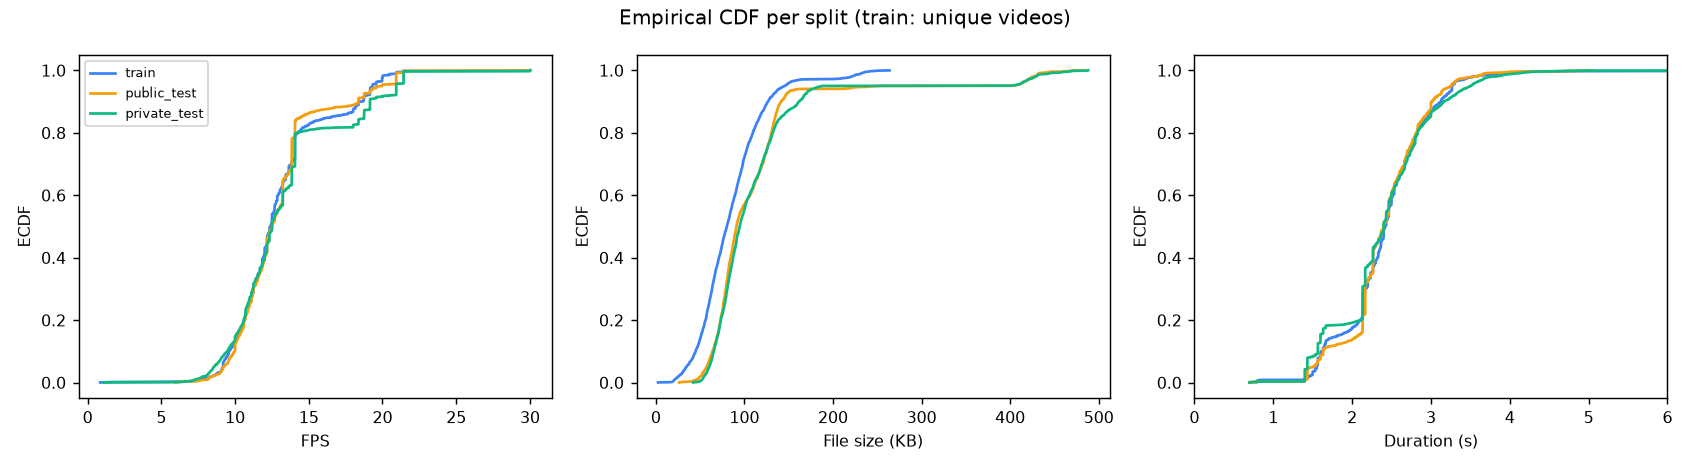
\includegraphics[width=\textwidth]{ecdf_by_split.png}
  \caption{Hàm phân phối tích luỹ thực nghiệm của FPS, dung lượng và thời lượng theo tập (train: video duy nhất). Đường dung lượng của train tách hẳn khỏi hai tập test.}
  \label{fig:eda_ecdf}
\end{figure}

Vì cỡ mẫu lớn nên mọi khác biệt dù nhỏ đều có $p$ rất bé; nhóm đánh giá chủ yếu theo độ lớn của $D$. Số khung hình giống nhau ở cả ba tập ($D<0{,}01$), độ phân giải cũng vậy. FPS, thời lượng và độ chuyển động khác biệt nhỏ ($D<0{,}1$). Riêng dung lượng khác biệt rõ giữa train và hai tập test ($D\approx0{,}23$--$0{,}24$), trong khi hai tập test gần nhau ($D\approx0{,}06$). Cụ thể:

\begin{itemize}
  \item \textbf{Dung lượng:} video test nặng hơn đáng kể (trung bình 113,6--116,3~KB so với 85,5~KB; trung vị 91,0--94,6~KB so với 80,6~KB). Tỷ lệ video vượt 167~KB (ngưỡng ngoại lai của train) là 3,1\% ở train nhưng 6,0\% ở public và 8,2\% ở private. Một phần chênh lệch có thể giải thích bởi khung đơn sắc (nén rất nhỏ) chỉ có ở train: trung vị dung lượng của video train có khung đơn sắc là 49,0~KB, còn của video train không có khung đơn sắc là 87,6~KB, gần mức của test. Tuy nhiên đuôi dài tới 488~KB ở test không xuất hiện ở train (lớn nhất 263,8~KB), cho thấy test có thể chứa các video chi tiết hoặc nhiễu hơn.
  \item \textbf{FPS:} trung vị gần như nhau (12,4 ở train, 12,5 ở hai tập test), nhưng private test có độ lệch chuẩn lớn hơn (3,69 so với 3,11 ở train) và đuôi dài hơn.
  \item \textbf{Khung đơn sắc:} khoảng 20\% video train nhưng gần như không có ở test (Bảng~\ref{tab:eda_solid}).
  \item \textbf{Người ký, nền, ánh sáng:} có thể khác giữa train và test; nhóm chưa định lượng được yếu tố này.
\end{itemize}

\noindent\textit{Hệ quả:} cần các phép tăng cường giúp mô hình bền vững với thay đổi màu sắc, độ sáng và khung cắt (\textit{ColorJitter}, \textit{Random Resized Crop}); việc loại bỏ khung đơn sắc ở train đồng thời giúp thu hẹp khoảng cách giữa phân phối train và test.

% =====================================================================
\subsubsection{Kết luận EDA và khuyến nghị cho bước tiền xử lý}
\label{subsec:eda_conclusion}

Bảng~\ref{tab:eda_reco} tổng hợp các vấn đề phát hiện được, bằng chứng và khuyến nghị cho bước tiền xử lý (Mục~\ref{sec:preprocess}) cũng như huấn luyện.

\begin{table}[H]
  \centering
  \caption{Tổng hợp vấn đề, bằng chứng và khuyến nghị cho bước tiền xử lý.}
  \label{tab:eda_reco}
  \small
  \begin{tabular}{@{}p{0.2\textwidth}p{0.36\textwidth}p{0.38\textwidth}@{}}
    \toprule
    \textbf{Vấn đề} & \textbf{Bằng chứng} & \textbf{Khuyến nghị} \\
    \midrule
    Tên lớp khác dạng Unicode & Khoá trong \texttt{label\_mapping.pkl} ở dạng NFD, thư mục lớp ở dạng NFC; 91/100 lớp không khớp nếu so nguyên văn & Chuẩn hoá NFC cả hai phía trước khi tra nhãn \\
    \addlinespace
    Video trùng lặp (\texttt{\_N}) & 1.069 tệp \texttt{\_N} giống hệt bản gốc; chỉ còn 2.776 video duy nhất & Khử trùng lặp theo MD5; chia train/validation theo ID gốc (bỏ hậu tố \texttt{\_N}) bằng \texttt{StratifiedGroupKFold} để tránh rò rỉ \\
    \addlinespace
    Mất cân bằng lớp & 6--74 video/lớp (sau khử trùng lặp: 5--51), 36/100 lớp có $\leq$25 video & Dùng Macro F1; trọng số lớp hoặc \texttt{WeightedRandomSampler}; oversample kèm tăng cường cho lớp ít mẫu; có thể dùng label smoothing \\
    \addlinespace
    Khung đơn sắc & 565/2.776 video duy nhất (20,4\%) chứa trung bình 12,2 khung đơn sắc; test gần như không có & Loại bỏ khung đơn sắc (độ lệch chuẩn điểm ảnh $<3$) \emph{trước} khi lấy mẫu $T=16$; nếu còn ít hơn 16 khung hợp lệ thì lặp khung \\
    \addlinespace
    Video rỗng & \texttt{Biết/214576}, \texttt{Khai báo/885339} (cùng 2 bản sao) đơn sắc toàn bộ & Loại khỏi tập huấn luyện \\
    \addlinespace
    Xung đột nhãn & 2 nhóm nội dung giống hệt nhưng thuộc \textit{Chậm lại} và \textit{Chào} & Xác minh nhãn đúng; nếu không xác minh được thì loại bỏ \\
    \addlinespace
    Độ dài không đồng nhất & 98,9\% video có 30 khung, tối thiểu 16 khung; thời lượng tới 35,3~s & Lấy mẫu $T=16$ khung đều bằng \texttt{linspace} \\
    \addlinespace
    FPS/dung lượng liên hệ với nhãn & $\eta^2\approx0{,}28$ (FPS), $0{,}15$ (dung lượng) giữa các lớp & Không dùng FPS, dung lượng làm đặc trưng; theo dõi nguy cơ shortcut \\
    \addlinespace
    Khác biệt miền train--test & Test nặng hơn (trung bình 114--116~KB so với 85,5~KB; KS $D\approx0{,}23$); khung đơn sắc chỉ có ở train & ColorJitter, Random Resized Crop, chuẩn hoá ImageNet; \emph{không} lật ngang \\
    \addlinespace
    Trùng train--public test & 157 video public giống hệt video train & Lưu ý khi diễn giải điểm public test \\
    \bottomrule
  \end{tabular}
\end{table}

Tóm lại, bộ dữ liệu có định dạng rất đồng nhất (100\% video $224\times224$, gần như đều 30 khung), nên khâu đọc và lấy mẫu khung đơn giản. Tuy nhiên dữ liệu huấn luyện có ba vấn đề cần xử lý trước khi huấn luyện: mất cân bằng lớp, khoảng 28\% tệp là bản sao gây nguy cơ rò rỉ dữ liệu, và khoảng 20\% video chứa khung đơn sắc vốn không xuất hiện ở dữ liệu kiểm tra. Đây là những yếu tố có thể khiến điểm validation cao hơn đáng kể so với điểm thực tế trên tập kiểm tra nếu không được xử lý.

\paragraph{Hạn chế của phân tích} FPS và thời lượng đọc từ metadata của container nên có thể không phản ánh tốc độ quay thực. Ngưỡng độ lệch chuẩn $<3$ chỉ phát hiện khung đơn sắc hoàn toàn, chưa phát hiện khung mờ hoặc chỉ có nền. Nhóm chưa định lượng sự khác biệt về người ký và bối cảnh giữa train và test, chưa xác định được nguyên nhân FPS liên hệ với nhãn, và chưa xác định được nhãn đúng cho các video xung đột.
]
% Cấu trúc theo khung EDA chuẩn:
%   3.1.1 Mục tiêu và tổng quan dữ liệu
%   3.1.2 Cấu trúc dữ liệu
%   3.1.3 Chất lượng dữ liệu
%   3.1.4 Phân tích đơn biến
%   3.1.5 Phân tích biến mục tiêu
%   3.1.6 Phân tích hai biến và đa biến
%   3.1.7 So sánh phân phối giữa các tập
%   3.1.8 Kết luận và khuyến nghị
% Gói cần: graphicx, booktabs, float, caption, amsmath
% =====================================================================

\subsection{Phân tích dữ liệu (EDA)}
\label{sec:eda}

% \edafile{thư mục}{tệp}: in đường dẫn script, cho phép xuống dòng sau dấu /
\newcommand{\edafile}[2]{\texttt{#1/}\allowbreak\texttt{#2}}
% Cho phép xuống dòng sau dấu gạch dưới trong tên tệp dài (vd. class\_counts\_train\_unique\_vs\_all.csv)
\let\edaOrigUS\_
\renewcommand{\_}{\edaOrigUS\allowbreak}
\sloppy

Mục này trình bày kết quả phân tích khám phá dữ liệu (\textit{Exploratory Data Analysis -- EDA}) trên bộ dữ liệu video ngôn ngữ ký hiệu. EDA chỉ nhằm \emph{quan sát} xu hướng, phân phối và chất lượng dữ liệu. Nhóm sử dụng Python làm công cụ để thực hiện EDA (\texttt{os}, \texttt{pickle}, \texttt{pandas}, \texttt{OpenCV}, \texttt{numpy}, \texttt{hashlib}, \texttt{matplotlib}).

Phần phân tích được tổ chức theo trình tự quy trình EDA: tổng quan và cấu trúc dữ liệu (Mục~\ref{subsec:eda_overview}--\ref{subsec:eda_structure}), chất lượng dữ liệu (Mục~\ref{subsec:eda_quality}), phân tích đơn biến (Mục~\ref{subsec:eda_uni}), phân tích biến mục tiêu (Mục~\ref{subsec:eda_class}), phân tích hai biến và đa biến (Mục~\ref{subsec:eda_multi}), so sánh giữa các tập (Mục~\ref{subsec:eda_shift}) và cuối cùng là kết luận kèm khuyến nghị (Mục~\ref{subsec:eda_conclusion}).

\begin{table}[H]
  \centering
  \caption{Các script EDA, thứ tự chạy và mục sử dụng kết quả.}
  \label{tab:eda_scripts}
  \small
  \begin{tabular}{@{}p{0.17\textwidth}p{0.26\textwidth}p{0.27\textwidth}p{0.18\textwidth}@{}}
    \toprule
    \textbf{Bước (thư mục)} & \textbf{Script -- câu hỏi} & \textbf{Kết quả chính} & \textbf{Dùng ở} \\
    \midrule
    \texttt{01\_overview} & \texttt{01\_scan\_metadata.py} -- dữ liệu gồm những gì? & \texttt{video\_metadata.csv} & 3.1.1 \\
      & \texttt{02\_dataset\_structure.py} -- chia tập, định dạng, tệp nhãn & \texttt{structure\_summary.txt} \newline \texttt{split\_sizes.png} & 3.1.2 \\
    \midrule
    \texttt{02\_data\_quality} & \texttt{01\_integrity\_missing.py} -- giá trị thiếu, tệp lỗi & \texttt{integrity\_summary.txt} & 3.1.3 \\
      & \texttt{02\_duplicates.py} -- trùng lặp, xung đột nhãn, trùng giữa các tập & \texttt{file\_hashes.csv} \newline \texttt{dups\_summary.txt} \newline \texttt{dedup\_summary.txt} \newline \texttt{class\_counts\_train\_unique\_vs\_all.csv} & 3.1.3, 3.1.5 \\
      & \texttt{03\_frame\_scan.py} -- quét nội dung từng khung & \texttt{video\_quality\_flags.csv} & 3.1.3, 3.1.6, 3.1.7 \\
      & \texttt{04\_frame\_quality\_summary.py} -- tổng hợp khung đơn sắc & \texttt{solid\_frame\_summary.txt} \newline \texttt{class\_solid\_frame\_ratio.csv} & 3.1.3, 3.1.6 \\
    \midrule
    \texttt{03\_univariate} & \texttt{01\_numeric\_attributes.py} -- phân phối, ngoại lai & \texttt{desc\_by\_split.csv} \newline \texttt{univariate\_summary.txt} \newline 3 histogram & 3.1.3, 3.1.4 \\
    \midrule
    \texttt{04\_target\_analysis} & \texttt{01\_class\_distribution.py} -- phân phối nhãn & \texttt{class\_summary.txt} \newline \texttt{class\_counts\_train.csv} \newline 3 hình & 3.1.5 \\
    \midrule
    \texttt{05\_bivariate\_multivariate} & \texttt{01\_correlation\_and\_label\_association.py} & \texttt{multivariate\_summary.txt} \newline 3 hình & 3.1.6 \\
    \midrule
    \texttt{06\_split\_comparison} & \texttt{01\_split\_shift.py} -- khác biệt phân phối giữa các tập & \texttt{split\_shift\_summary.txt} \newline \texttt{ecdf\_by\_split.png} & 3.1.7 \\
    \midrule
    \texttt{07\_visual\_inspection} & \texttt{01\_sample\_frames.py} -- khung hình mẫu & 2 lưới khung hình & 3.1.2 \\
      & \texttt{02\_flagged\_videos.py} -- xem lại video bị đánh dấu & \texttt{flagged\_videos\_info.txt} \newline 2 hình & 3.1.3 \\
    \bottomrule
  \end{tabular}
\end{table}

% =====================================================================
\subsubsection{Mục tiêu và tổng quan dữ liệu}
\label{subsec:eda_overview}

\paragraph{Bài toán và thước đo} Bài toán là phân loại video ngôn ngữ ký hiệu (\textit{Sign Language Video Classification}) thành $N=100$ lớp từ vựng tiếng Việt. Đầu vào là một video ghi cử chỉ của một người, được tiền xử lý thành chuỗi $T=16$ khung hình RGB; đầu ra là nhãn dự đoán. Thước đo chính thức là Macro F1-Score. Biến mục tiêu là nhãn lớp (biến phân loại, 100 giá trị), còn các thuộc tính mô tả video (số khung hình, FPS, dung lượng\ldots) chỉ đóng vai trò thông tin phụ trợ cho phân tích.

\paragraph{Nguồn dữ liệu} Bộ dữ liệu là đề chính thức của cuộc thi \textit{Olympic Trí tuệ Nhân tạo Sinh viên 2025 -- Vòng Sơ loại} do Khoa Trí tuệ Nhân tạo, Học viện Công nghệ Bưu chính Viễn thông (PTIT) tổ chức. Các lớp thuộc nhiều nhóm chủ đề: y tế -- dịch bệnh (\textit{Bệnh viện}, \textit{Cách ly}, \textit{Khẩu trang}, \textit{Virus}, \textit{Sốt}, \textit{Ho}\ldots), cảm xúc (\textit{Lo lắng}, \textit{Xúc động}, \textit{Thương}, \textit{Ghét}\ldots), hành động thường ngày (\textit{Ăn}, \textit{Uống}, \textit{Chạy}, \textit{Đi}, \textit{Mua}\ldots), thời gian -- vị trí (\textit{Ban ngày}, \textit{Trưa}, \textit{Hôm nay}, \textit{Phía sau}, \textit{Rẽ trái}\ldots) và phương tiện (\textit{Ô tô}, \textit{Xe máy}, \textit{Xe đạp}).

\paragraph{Từ điển dữ liệu} Vì dữ liệu là video nên không có bảng thuộc tính sẵn. Nhóm duyệt cây thư mục, mở từng video bằng \texttt{cv2.VideoCapture} và gom thông tin vào một bảng metadata duy nhất (\texttt{01\_overview/video\_metadata.csv}, 8.364 dòng). Mã băm MD5 được lưu ở \texttt{02\_data\_quality/file\_hashes.csv}, còn các thuộc tính suy ra từ nội dung khung hình (khung đơn sắc, chuyển động) được lưu ở \texttt{02\_data\_quality/video\_quality\_flags.csv}. Ba bảng có chung khoá (tập, lớp, tên tệp). Bảng~\ref{tab:eda_dict} liệt kê ý nghĩa từng thuộc tính; mọi thống kê phía sau chỉ là phép ghép và \texttt{groupby} trên ba bảng này.

\begin{table}[H]
  \centering
  \caption{Từ điển các thuộc tính dùng trong phân tích.}
  \label{tab:eda_dict}
  \small
  \begin{tabular}{@{}p{0.22\textwidth}p{0.17\textwidth}p{0.5\textwidth}@{}}
    \toprule
    \textbf{Thuộc tính} & \textbf{Kiểu} & \textbf{Ý nghĩa / cách tính} \\
    \midrule
    \texttt{split}        & phân loại & Tập chứa video: \texttt{train}, \texttt{public\_test}, \texttt{private\_test} \\
    \texttt{cls}          & phân loại & Nhãn lớp, lấy từ tên thư mục con của \texttt{train} (không có ở hai tập test) \\
    \texttt{file}         & chuỗi     & Tên tệp \texttt{.mp4}; hậu tố \texttt{\_N} biểu thị bản sao \\
    \texttt{frames}       & số nguyên & Số khung hình (\texttt{CAP\_\allowbreak PROP\_\allowbreak FRAME\_\allowbreak COUNT}) \\
    \texttt{fps}          & số thực   & Tốc độ khung hình ghi trong container \\
    \texttt{w}, \texttt{h}& số nguyên & Chiều rộng, chiều cao khung hình (pixel) \\
    \texttt{dur}          & số thực   & Thời lượng (giây) $=\texttt{frames}/\texttt{fps}$ \\
    \texttt{size\_kb}     & số thực   & Dung lượng tệp (KB) \\
    \texttt{md5}          & chuỗi     & Mã băm nội dung tệp, dùng phát hiện video trùng (lưu trong \texttt{file\_hashes.csv}) \\
    \texttt{solid\_ratio} & số thực   & Tỷ lệ khung đơn sắc trong video (khung có độ lệch chuẩn điểm ảnh $<3$) \\
    \texttt{motion}       & số thực   & Độ chuyển động trung bình $\overline{|f_t-f_{t-1}|}$ giữa các khung liên tiếp (ảnh xám) \\
    \bottomrule
  \end{tabular}
\end{table}

% =====================================================================
\subsubsection{Cấu trúc dữ liệu}
\label{subsec:eda_structure}

\paragraph{Quy mô và cách chia} Sau khi giải nén \texttt{dataset.zip} (khoảng 864~MB), dữ liệu gồm ba tập video và một tệp ánh xạ nhãn (Bảng~\ref{tab:eda_splits}, Hình~\ref{fig:eda_split_sizes}). Tệp \texttt{label\_mapping.pkl} là một \texttt{dict[str, int]} chứa đúng 100 lớp, đánh chỉ số 0--99 theo thứ tự bảng chữ cái tiếng Việt (\textit{An ủi}~$=0$, \textit{Áp dụng}~$=1$, \textit{Ăn}~$=2$, \ldots, \textit{Đồng ý}~$=99$). Khi đối chiếu với tên thư mục lớp, nhóm phát hiện hai bên dùng \emph{hai dạng chuẩn hoá Unicode khác nhau}: khoá trong \texttt{label\_mapping.pkl} ở dạng NFD (dấu tách rời khỏi chữ cái), còn tên thư mục ở dạng NFC (dấu dựng sẵn). Vì vậy 91/100 tên lớp (mọi lớp có dấu) không khớp nếu so nguyên văn, dù hiển thị giống hệt nhau; sau khi chuẩn hoá cả hai về NFC thì 100 lớp khớp hoàn toàn và chỉ số liên tục 0--99 không trùng.

\begin{table}[H]
  \centering
  \caption{Cấu trúc và quy mô các tập dữ liệu.}
  \label{tab:eda_splits}
  \begin{tabular}{@{}lp{0.42\textwidth}rr@{}}
    \toprule
    \textbf{Thành phần} & \textbf{Nội dung} & \textbf{Số video} & \textbf{Dung lượng} \\
    \midrule
    \texttt{train/}         & 100 thư mục con, mỗi thư mục là một lớp (có nhãn) & 3.875 & 323~MB \\
    \texttt{public\_test/}  & Video không nhãn, dùng cho bảng xếp hạng công khai & 1.630 & 181~MB \\
    \texttt{private\_test/} & Video không nhãn, dùng cho xếp hạng cuối cùng      & 2.859 & 325~MB \\
    \texttt{label\_mapping.pkl} & \texttt{dict[str, int]}: tên lớp (Unicode NFD) $\rightarrow$ chỉ số 0--99 & -- & -- \\
    \midrule
    \textbf{Tổng} & & \textbf{8.364} & $\approx$\textbf{829~MB} \\
    \bottomrule
  \end{tabular}
\end{table}

\begin{figure}[H]
  \centering
  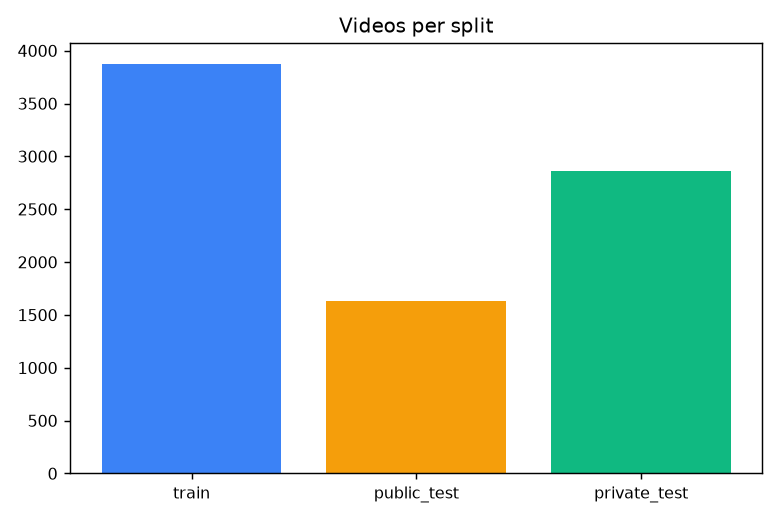
\includegraphics[width=0.6\textwidth]{split_sizes.png}
  \caption{Số lượng video trong ba tập \texttt{train}, \texttt{public\_test} và \texttt{private\_test}.}
  \label{fig:eda_split_sizes}
\end{figure}

\paragraph{Định dạng video} Toàn bộ 8.364 tệp đều là \texttt{.mp4} và đọc được; không có video nào có 0 khung hình. Độ phân giải đồng nhất tuyệt đối: 100\% video ở cả ba tập đều là $224\times224$ (Bảng~\ref{tab:eda_res}). Số khung hình gần như cố định ở mức 30 (chi tiết ở Mục~\ref{subsec:eda_uni}).

\begin{table}[H]
  \centering
  \caption{Thống kê độ phân giải video.}
  \label{tab:eda_res}
  \begin{tabular}{@{}lrrr@{}}
    \toprule
    \textbf{Tập} & \textbf{Độ phân giải} & \textbf{Số video} & \textbf{Tỷ lệ} \\
    \midrule
    train         & $224\times224$ & 3.875 & 100\% \\
    public\_test  & $224\times224$ & 1.630 & 100\% \\
    private\_test & $224\times224$ & 2.859 & 100\% \\
    \bottomrule
  \end{tabular}
\end{table}

\paragraph{Quan sát trực quan} Để kiểm chứng bằng mắt, nhóm trích 6--8 khung hình phân bố đều trong video (\texttt{cap.set(cv2.CAP\_\allowbreak PROP\_\allowbreak POS\_\allowbreak FRAMES, i)} với $i$ lấy từ \texttt{np.linspace}) và ghép thành lưới ảnh cho một số lớp (Hình~\ref{fig:eda_samples}). Các video được quay chính diện, người ký ngồi hoặc đứng giữa khung hình, thấy rõ phần thân trên, hai tay và khuôn mặt; nền chủ yếu là tường trơn với ánh sáng trong nhà. Sự đa dạng nằm ở người ký (giới tính, trang phục, kính), màu nền (be, xanh nhạt, trắng) và vị trí tay lúc bắt đầu. Ký hiệu thường chỉ chiếm một phần thời lượng: các khung đầu và cuối thường là tư thế nghỉ. Ở một số video xuất hiện các khung \emph{đơn sắc hoàn toàn} (hàng \textit{Phỏng vấn}, \textit{Uống}); hiện tượng này được định lượng ở Mục~\ref{subsec:eda_quality}.

\begin{figure}[H]
  \centering
  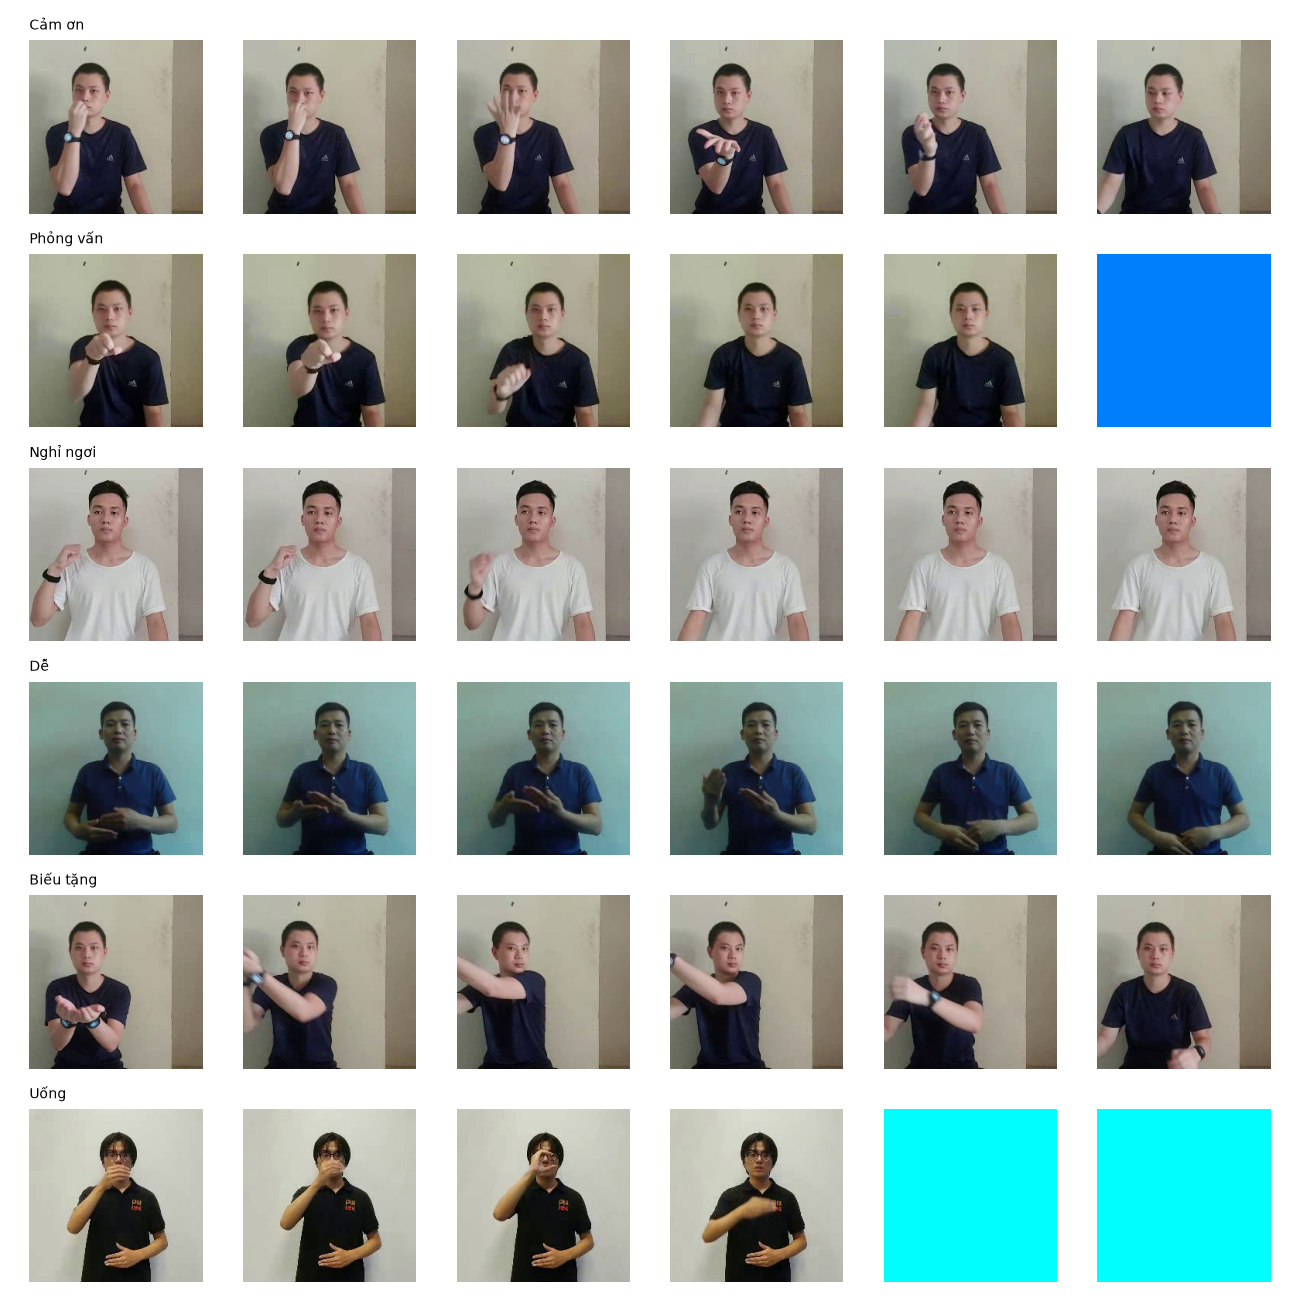
\includegraphics[width=0.85\textwidth]{sample_frames_6classes.png}
  \caption{Khung hình mẫu (lấy đều theo thời gian) của sáu lớp. Hàng \textit{Phỏng vấn} và \textit{Uống} có các khung đơn sắc ở cuối video.}
  \label{fig:eda_samples}
\end{figure}

\noindent\textit{Hệ quả:} khi gán nhãn số cho video phải chuẩn hoá tên lớp bằng \texttt{unicodedata.normalize(\textquotesingle NFC\textquotesingle, ...)} trước khi tra \texttt{label\_mapping.pkl}, nếu không phần lớn video sẽ không tìm được nhãn. Chỉ có tập \texttt{train} mang nhãn nên tập kiểm định (\textit{validation}) phải tách ra từ chính tập này; việc tách cần tính đến trùng lặp (Mục~\ref{subsec:eda_quality}). Thông tin phân biệt nằm ở hình dạng và chuyển động của bàn tay, khẩu hình và tư thế, nên các phép tăng cường không được làm đổi ngữ nghĩa không gian; đặc biệt \emph{không} dùng lật ngang (\textit{Horizontal Flip}) vì có thể đổi nghĩa tay trái/phải.

% =====================================================================
\subsubsection{Chất lượng dữ liệu}
\label{subsec:eda_quality}

\paragraph{Script và cách thực hiện}
\begin{itemize}
  \item \textbf{Script:} bốn script trong \texttt{02\_data\_quality/}, chạy theo thứ tự: \edafile{02\_data\_quality}{01\_integrity\_missing.py}, \edafile{02\_data\_quality}{02\_duplicates.py}, \edafile{02\_data\_quality}{03\_frame\_scan.py}, \edafile{02\_data\_quality}{04\_frame\_quality\_summary.py}. Kiểm tra bằng mắt dùng \edafile{07\_visual\_inspection}{02\_flagged\_videos.py}.
  \item \textbf{Cách khai thác dữ liệu:} 
  
  (i) \emph{Giá trị thiếu và lỗi đọc:} \texttt{01\_integrity\_missing.py} đếm ô trống (\texttt{isna}) theo cột và theo tập, đếm video có 0 khung, FPS hoặc kích thước bằng 0, rồi liệt kê các tệp có giá trị phi lý theo ngưỡng tuyệt đối (dưới 10~KB, dưới 16 khung, FPS dưới 5). 
  
  (ii) \emph{Trùng lặp:} \texttt{02\_duplicates.py} đọc toàn bộ byte của từng tệp, tính \texttt{hashlib.md5} một lần và lưu vào \texttt{file\_hashes.csv}; hai tệp cùng mã băm là cùng nội dung. Gom nhóm theo mã băm để đếm bản sao, tìm nhóm có nhiều hơn một nhãn (xung đột nhãn), lấy giao các tập mã băm giữa train, public test, private test, rồi giữ một tệp cho mỗi mã băm và đếm lại số video mỗi lớp. 
  
  (iii) \emph{Khung đơn sắc:} \texttt{03\_frame\_scan.py} giải mã \emph{từng} khung bằng \texttt{cap.read()}, tính độ lệch chuẩn điểm ảnh của từng kênh màu và coi khung là đơn sắc khi giá trị lớn nhất nhỏ hơn 3; đồng thời đếm số khung đơn sắc liên tiếp ở đầu video và tính độ chuyển động là trung bình $|f_t-f_{t-1}|$ trên ảnh xám. \texttt{04\_frame\_quality\_summary.py} đối chiếu số khung đọc được với metadata, bỏ các bản sao \texttt{\_N}, phân loại vị trí khung đơn sắc (đầu, cuối, giữa, toàn bộ) và mô phỏng việc lấy $T=16$ khung bằng \texttt{np.linspace} để đếm số khung đơn sắc bị lấy trúng. 
  
  (iv) \emph{Kiểm tra bằng mắt:} \texttt{02\_flagged\_videos.py} \emph{tự chọn} video cần xem từ kết quả hai bước trên, không dùng danh sách chọn tay. Tiêu chí chọn gồm: 6 video có tỷ lệ khung đơn sắc cao nhất trong số các video có từ 50\% khung đơn sắc trở lên; mọi video thuộc nhóm MD5 nằm ở hơn một lớp; một ví dụ cho mỗi dạng xuất hiện khung đơn sắc. Ngoại lai theo quy tắc Tukey được tính ở bước đơn biến (Mục~\ref{subsec:eda_uni}).
  \item \textbf{Đầu ra:} \texttt{integrity\_summary.txt}, \texttt{file\_hashes.csv}, \texttt{dups\_summary.txt}, \texttt{dedup\_summary.txt}, \texttt{class\_counts\_train\_unique\_vs\_all.csv}, \texttt{video\_quality\_flags.csv}, \texttt{solid\_frame\_summary.txt}, \texttt{class\_solid\_frame\_ratio.csv}; ở bước kiểm tra bằng mắt là \texttt{flagged\_videos\_info.txt}, \texttt{flagged\_videos\_check.png}, \texttt{solid\_frame\_patterns.png}.
\end{itemize}

Nhóm kiểm tra chất lượng dữ liệu theo các khía cạnh: giá trị thiếu, bản ghi trùng lặp, khung hình đơn sắc/video rỗng, giá trị ngoại lai, nhiễu nhãn và trùng lặp giữa các tập. Bảng~\ref{tab:eda_quality} tóm tắt các vấn đề phát hiện được.

\begin{table}[H]
  \centering
  \caption{Tóm tắt các vấn đề chất lượng dữ liệu.}
  \label{tab:eda_quality}
  \small
  \begin{tabular}{@{}p{0.26\textwidth}p{0.36\textwidth}p{0.30\textwidth}@{}}
    \toprule
    \textbf{Vấn đề} & \textbf{Số lượng} & \textbf{Ví dụ} \\
    \midrule
    Bản sao hậu tố \texttt{\_N} trong train & 1.069 tệp giống hệt bản gốc; còn 2.776 video duy nhất & \texttt{127824.mp4}, \texttt{127824\_1.mp4}, \texttt{127824\_2.mp4} \\
    Video có khung đơn sắc (train) & 758/3.875 tệp; 565/2.776 video duy nhất (20,4\%), ở 78/100 lớp & \texttt{Thất lạc/708519}, \texttt{Bộ y tế/523389} \\
    Video rỗng hoàn toàn & 2 video gốc (4 tệp kể cả bản sao) & \texttt{Biết/214576}, \texttt{Khai báo/885339} \\
    Nhiễu nhãn (cùng nội dung, khác lớp) & 2 nhóm nội dung, 5 tệp & \textit{Chậm lại} $\leftrightarrow$ \textit{Chào} \\
    Trùng train $\rightarrow$ public test & 157 video public giống hệt video train & -- \\
    Trùng public $\leftrightarrow$ private & 896 video & -- \\
    \bottomrule
  \end{tabular}
\end{table}

\paragraph{Giá trị thiếu và lỗi đọc} Bảng metadata không có giá trị thiếu ở bất kỳ thuộc tính nào (nhãn \texttt{cls} chỉ trống ở hai tập test vì các tập này vốn không có nhãn). Mọi video đều mở và giải mã được, và ở cả 8.364 video, số khung giải mã thực tế khớp với số khung ghi trong metadata. Như vậy không có vấn đề về tệp hỏng hay nhãn bị thiếu ở tập train.

\paragraph{Trùng lặp trong tập train} Nhóm tính mã băm MD5 nội dung từng tệp (\texttt{hashlib.md5}) rồi gom nhóm theo mã băm. Có 1.069/3.875 tệp mang hậu tố \texttt{\_1}, \texttt{\_2}, \texttt{\_3}\ldots{} So sánh từng cặp cho thấy cả 1.069 tệp này đều có bản gốc tồn tại, cùng lớp và \emph{giống hệt bản gốc từng byte} (cùng số khung, FPS, dung lượng): đây là bản sao, không phải biến thể tăng cường. Có 176 video gốc có 1 bản sao, 169 video có 2 và 185 video có 3. Tính cả các bản sao khác, tập train có 1.099 tệp dư thừa và chỉ còn \textbf{2.776 video duy nhất}. Các bản sao tập trung ở những lớp vốn đã nhiều mẫu (\textit{Chậm lại} và \textit{Trường học} cùng thêm 25 tệp, \textit{Rau} và \textit{Nhìn} thêm 23, \textit{Khóc} thêm 22\ldots), nên sau khi khử trùng lặp số video mỗi lớp còn từ 5 đến 51 (trung bình 27,8; tỷ lệ chênh $\approx$10,2 lần). Bảng trước/sau khử trùng lặp của từng lớp lưu ở \texttt{class\_counts\_train\_unique\_vs\_all.csv}. Hệ quả là nguy cơ rò rỉ dữ liệu (\textit{Data Leakage}): nếu chia train/validation ngẫu nhiên theo từng tệp, các bản sao của cùng một video rơi vào cả hai phần, làm điểm validation bị thổi phồng.

\paragraph{Khung hình đơn sắc và video rỗng} Nhóm đọc \emph{toàn bộ} khung hình của 8.364 video và tính độ lệch chuẩn giá trị điểm ảnh trên từng kênh màu; khung có độ lệch chuẩn lớn nhất giữa ba kênh nhỏ hơn 3 được coi là \emph{khung đơn sắc}. Kết quả tổng hợp ở Bảng~\ref{tab:eda_solid}.

\begin{table}[H]
  \centering
  \caption{Số video chứa khung hình đơn sắc theo từng tập.}
  \label{tab:eda_solid}
  \begin{tabular}{@{}lrrrr@{}}
    \toprule
    \textbf{Tập} & \textbf{Tổng video} & \textbf{Có $\geq$1 khung đơn sắc} & \textbf{Đơn sắc toàn bộ} & \textbf{Tỷ lệ} \\
    \midrule
    train (tất cả tệp)        & 3.875 & 758 & 4 & 19,6\% \\
    train (video duy nhất)    & 2.776 & 565 & 2 & 20,4\% \\
    public\_test              & 1.630 & 1   & 0 & 0,06\% \\
    private\_test             & 2.859 & 1   & 0 & 0,03\% \\
    \bottomrule
  \end{tabular}
\end{table}

Đây là phát hiện đáng chú ý nhất của EDA. Khoảng một phần năm số video duy nhất trong train (565/2.776, thuộc 78/100 lớp) chứa khung đơn sắc, và số khung này không nhỏ: trung bình 12,2 khung trên khoảng 30 khung mỗi video (trung vị 12, nhiều nhất 23). Các khung có màu thuần (đỏ, xanh lục, xanh lam, xanh lục lam, tím, vàng, trắng, đen, xám) và xuất hiện theo các dạng: chỉ ở đầu video (231 video), chỉ ở cuối (161), cả đầu và cuối (116), xen ở giữa (55) hoặc toàn bộ video (2) (Hình~\ref{fig:eda_solid_examples}). Lớp có tỷ lệ video bị ảnh hưởng cao nhất là \textit{Có thể} (6/15 video duy nhất), \textit{Xin lỗi} (5/14) và \textit{Thất lạc} (7/20) (chi tiết ở \texttt{class\_solid\_frame\_ratio.csv}).

\begin{figure}[H]
  \centering
  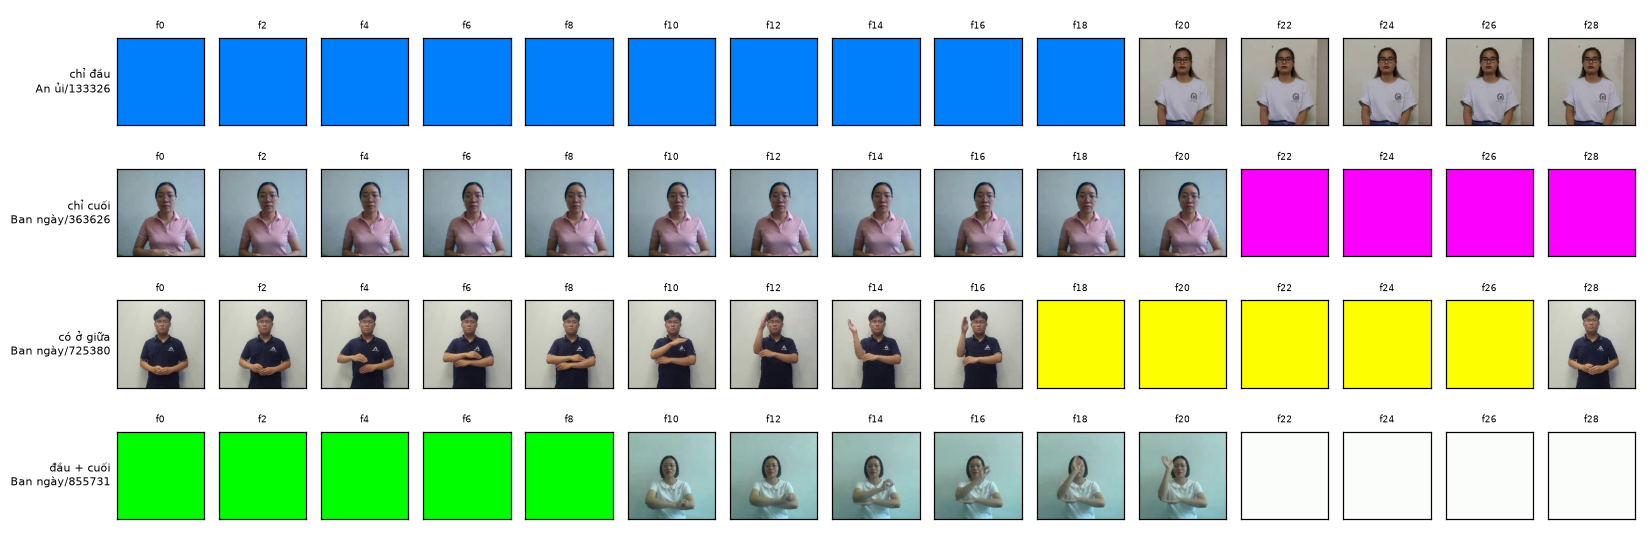
\includegraphics[width=\textwidth]{solid_frame_patterns.png}
  \caption{Bốn dạng khung đơn sắc trong tập train (khung chẵn $f_0$--$f_{28}$), mỗi dạng một video được chọn tự động: chỉ ở đầu (\textit{An ủi}/133326), chỉ ở cuối (\textit{Ban ngày}/363626), xen ở giữa (\textit{Ban ngày}/725380), cả đầu và cuối (\textit{Ban ngày}/855731).}
  \label{fig:eda_solid_examples}
\end{figure}

Hiện tượng này ảnh hưởng trực tiếp đến cách lấy mẫu: khi lấy $T=16$ khung đều nhau bằng \texttt{linspace} trên 565 video nói trên, trung bình có 6,4/16 khung được chọn là khung đơn sắc, và ở 224 video có từ 8/16 khung trở lên (ít nhất một nửa chuỗi đầu vào) là khung đơn sắc. Ngược lại, mỗi tập test chỉ có 1 video chứa đúng 1 khung đơn sắc. Như vậy khung đơn sắc là đặc điểm \emph{riêng của tập train}: nếu không xử lý, mô hình vừa mất thông tin ký hiệu, vừa có thể học các tín hiệu giả không tồn tại ở dữ liệu kiểm tra.

Sáu hàng đầu của Hình~\ref{fig:eda_suspicious} là các video có tỷ lệ khung đơn sắc cao nhất. Hai video được xác nhận bằng mắt là \textbf{rỗng hoàn toàn}: \texttt{Biết/214576.mp4} (2,5~KB, 16 khung, toàn màu xanh lục) và \texttt{Khai báo/885339.mp4} (2,7~KB, 23 khung, toàn màu xanh lam, kèm 2 bản sao \texttt{\_1}, \texttt{\_2}); cả hai không có người ký. Bốn video tiếp theo có 20--21/30 khung đơn sắc: \texttt{Nôn ói/915809}, \texttt{Thất lạc/708519}, \texttt{Chân/984642} và \texttt{Khai báo/362529}. Người ký chỉ xuất hiện trong khoảng 10 khung, ví dụ \texttt{Khai báo/362529} có 20 khung đỏ đầu tiên ($f_0$--$f_{19}$).

\paragraph{Giá trị ngoại lai} Nhóm dùng quy tắc Tukey (ngoài khoảng $[Q_1-1{,}5\,\mathrm{IQR},\,Q_3+1{,}5\,\mathrm{IQR}]$ tính trên tập train) cho thời lượng, dung lượng và FPS. Số lượng ngoại lai khá nhiều nhưng phần lớn chỉ lệch nhẹ (Mục~\ref{subsec:eda_uni}). Đáng chú ý là các ngoại lai cực đoan: thời lượng trên 5~s có 10 video train, 1 video public test và 3 video private test (lớn nhất 35,3~s ở train, 28,1~s ở private test); FPS dưới 5 có 9 video train và 2 video private test; dung lượng dưới 10~KB có 4 tệp train, đều là các video rỗng nói trên. Các ngoại lai này không nhất thiết là lỗi mà phản ánh việc video được lấy mẫu lại về $\approx$30 khung từ các clip gốc có độ dài rất khác nhau.

\paragraph{Nhiễu nhãn} Khi gom nhóm theo MD5, có hai nhóm nội dung giống hệt nhau nhưng nằm ở \emph{hai lớp khác nhau}: \texttt{Chậm lại/284430.mp4} trùng với \texttt{Chào/392683.mp4} và \texttt{Chào/468203.mp4}; \texttt{Chậm lại/254739.mp4} trùng với \texttt{Chào/792094.mp4}. Nhóm đã xem trực tiếp (Hình~\ref{fig:eda_suspicious}, năm hàng cuối) và xác nhận chúng có cùng người ký, cùng chuỗi động tác. Một video không thể đồng thời mang hai nghĩa nên ít nhất một trong hai nhãn là sai; tuy nhiên việc xác định nhãn đúng cần người am hiểu ngôn ngữ ký hiệu Việt Nam, nên báo cáo chỉ ghi nhận đây là \emph{xung đột nhãn}.

\begin{figure}[H]
  \centering
  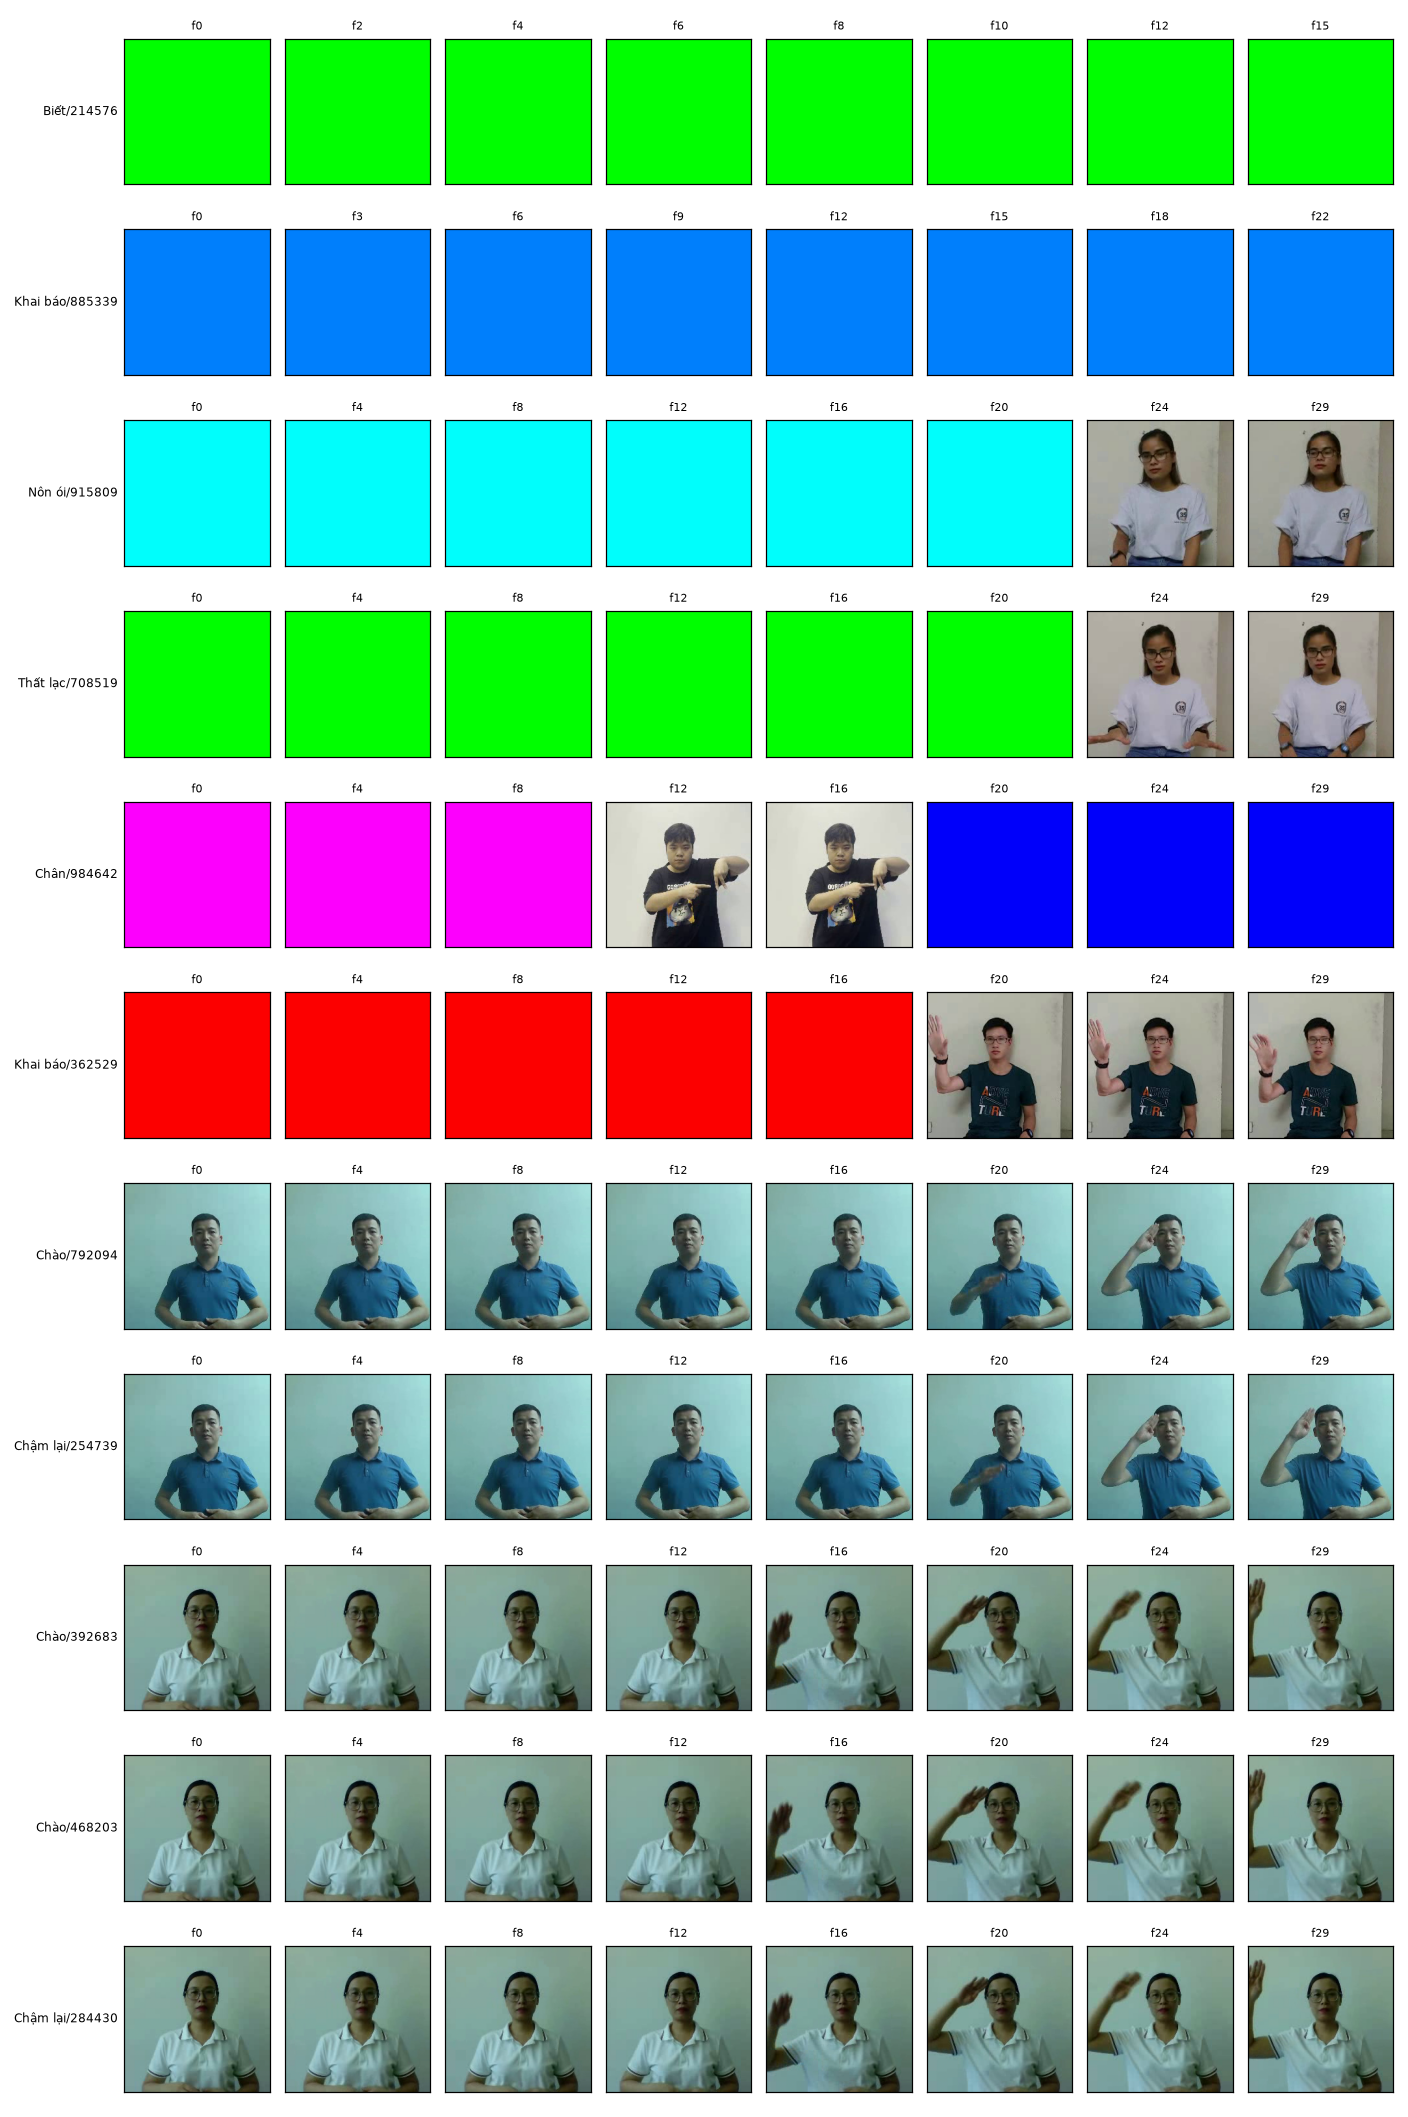
\includegraphics[width=0.9\textwidth,height=0.72\textheight,keepaspectratio]{flagged_videos_check.png}
  \caption{Kiểm tra bằng mắt các video do bước kiểm tra chất lượng tự đánh dấu. Sáu hàng đầu là các video có tỷ lệ khung đơn sắc cao nhất, gồm hai video rỗng hoàn toàn (\textit{Biết}/214576, \textit{Khai báo}/885339). Năm hàng cuối là hai nhóm video trùng nội dung nhưng khác nhãn (\textit{Chậm lại} $\leftrightarrow$ \textit{Chào}).}
  \label{fig:eda_suspicious}
\end{figure}

\paragraph{Trùng lặp giữa các tập} Public test có 8 bản trùng nội bộ (1.622 video duy nhất) và \textbf{157 video giống hệt video trong train}; private test có 2.782 video duy nhất, không trùng với train, nhưng có 896 video trùng với public test. Ngoài ra, 2.806 tên tệp trong private test trùng với tên tệp trong train nhưng nội dung hoàn toàn khác (MD5 khác, chênh lệch điểm ảnh lớn), nên đây chỉ là trùng cách đặt mã số; nguyên nhân chưa rõ và tên tệp \emph{không} được dùng để suy luận nhãn.

\noindent\textit{Hệ quả:} dữ liệu train chưa sạch; trước khi huấn luyện cần khử trùng lặp, loại video rỗng, xử lý khung đơn sắc và rà soát các nhãn xung đột. Điểm trên public test có thể bị ảnh hưởng một phần bởi 157 video đã có trong train.

% =====================================================================
\subsubsection{Phân tích đơn biến}
\label{subsec:eda_uni}

\paragraph{Script và cách thực hiện}
\begin{itemize}
  \item \textbf{Script:} \edafile{03\_univariate}{01\_numeric\_attributes.py}.
  \item \textbf{Cách khai thác dữ liệu:} với mỗi thuộc tính số (\texttt{frames}, \texttt{fps}, \texttt{dur}, \texttt{size\_kb}), script tính \texttt{groupby(\textquotesingle split\textquotesingle).describe()} (trung bình, độ lệch chuẩn, min, các tứ phân vị, max), hệ số lệch (\textit{skewness}) và các giá trị phổ biến nhất. Ngoại lai được xác định theo quy tắc Tukey với ngưỡng tính trên train rồi áp lên cả ba tập. Script vẽ histogram của từng thuộc tính cho ba tập trên cùng trục; histogram FPS và dung lượng dùng mật độ (\texttt{density=True}) để so sánh được các tập có kích thước khác nhau.
  \item \textbf{Đầu ra:} \texttt{desc\_by\_split.csv} (Bảng~\ref{tab:eda_desc}), \texttt{univariate\_summary.txt}, \texttt{frames\_hist\_by\_split.png}, \texttt{fps\_hist\_by\_split.png}, \texttt{filesize\_hist\_by\_split.png}.
\end{itemize}

Mục này khảo sát phân phối của từng thuộc tính số: số khung hình, FPS, thời lượng và dung lượng, tính trên từng tập (Bảng~\ref{tab:eda_desc}). Độ phân giải đã được trình bày ở Bảng~\ref{tab:eda_res}.

\begin{table}[H]
  \centering
  \caption{Thống kê mô tả các thuộc tính số theo từng tập.}
  \label{tab:eda_desc}
  \small
  \begin{tabular}{@{}llrrrrrrr@{}}
    \toprule
    \textbf{Thuộc tính} & \textbf{Tập} & \textbf{Mean} & \textbf{Std} & \textbf{Min} & \textbf{Q1} & \textbf{Median} & \textbf{Q3} & \textbf{Max} \\
    \midrule
    \multirow{3}{*}{Số khung}
      & train   & 29,88 & 1,26 & 16 & 30 & 30 & 30 & 30 \\
      & public  & 29,96 & 0,66 & 16 & 30 & 30 & 30 & 30 \\
      & private & 29,98 & 0,44 & 21 & 30 & 30 & 30 & 30 \\
    \midrule
    \multirow{3}{*}{FPS}
      & train   & 12,94 & 3,11 & 0,85 & 10,98 & 12,34 & 14,06 & 30,02 \\
      & public  & 12,97 & 3,00 & 5,93 & 10,98 & 12,50 & 13,85 & 30,00 \\
      & private & 13,32 & 3,69 & 1,07 & 10,84 & 12,50 & 14,06 & 30,02 \\
    \midrule
    \multirow{3}{*}{Thời lượng (s)}
      & train   & 2,48 & 1,36 & 0,70 & 2,13 & 2,43 & 2,73 & 35,29 \\
      & public  & 2,42 & 0,51 & 0,70 & 2,17 & 2,40 & 2,73 & 5,06 \\
      & private & 2,42 & 0,82 & 0,70 & 2,13 & 2,40 & 2,77 & 28,14 \\
    \midrule
    \multirow{3}{*}{Dung lượng (KB)}
      & train   & 85,5  & 38,5 & 2,5  & 60,2 & 80,6 & 103,0 & 263,8 \\
      & public  & 113,6 & 77,5 & 26,2 & 76,1 & 91,0 & 125,8 & 483,2 \\
      & private & 116,3 & 77,7 & 42,2 & 77,7 & 94,6 & 126,0 & 488,0 \\
    \bottomrule
  \end{tabular}
\end{table}

\paragraph{Số khung hình} Hầu hết video có đúng 30 khung: 3.832/3.875 video train (98,9\%), 1.623/1.630 public test và 2.850/2.859 private test; ở train có 26 video chỉ có 16 khung. Không video nào ngắn hơn 16 khung (Hình~\ref{fig:eda_frames_hist}), nên không cần đệm khung thực sự khi lấy $T=16$.

\begin{figure}[H]
  \centering
  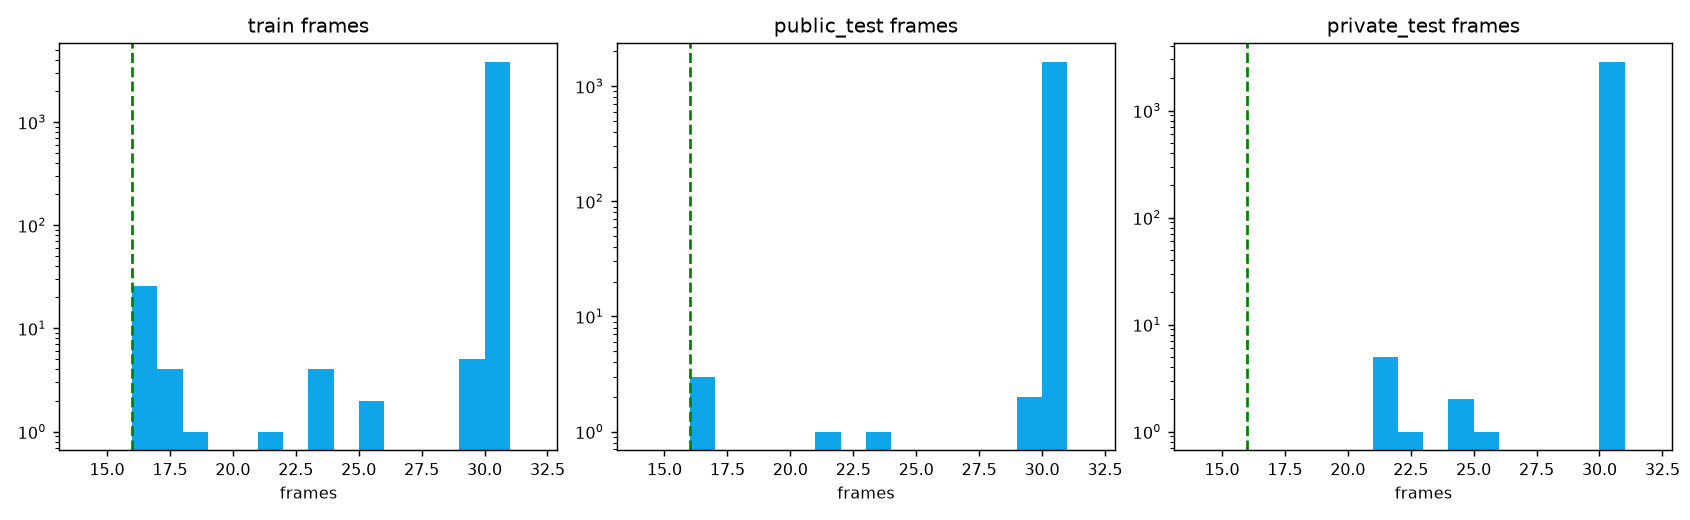
\includegraphics[width=\textwidth]{frames_hist_by_split.png}
  \caption{Histogram số khung hình mỗi video theo tập (trục tung thang log). Đường đứt nét đánh dấu $T=16$.}
  \label{fig:eda_frames_hist}
\end{figure}

\paragraph{FPS và thời lượng} Dù số khung gần như cố định, FPS biến thiên mạnh: train có 961 giá trị FPS khác nhau, từ 0,85 đến 30,02 (trung vị 12,3), phân phối lệch phải với đuôi dài (hệ số lệch 1,01 ở train; Hình~\ref{fig:eda_fps_hist}). Vì thời lượng $=\texttt{frames}/\texttt{fps}$ nên thời lượng thực của cùng 30 khung dao động lớn: trung vị khoảng 2,4~s nhưng có video tới 35,3~s ở train và 28,1~s ở private test, trong khi 99\% video đều ngắn hơn khoảng 4~s. Điều này cho thấy video đã được lấy mẫu lại về khoảng 30 khung bất kể độ dài clip gốc.

\begin{figure}[H]
  \centering
  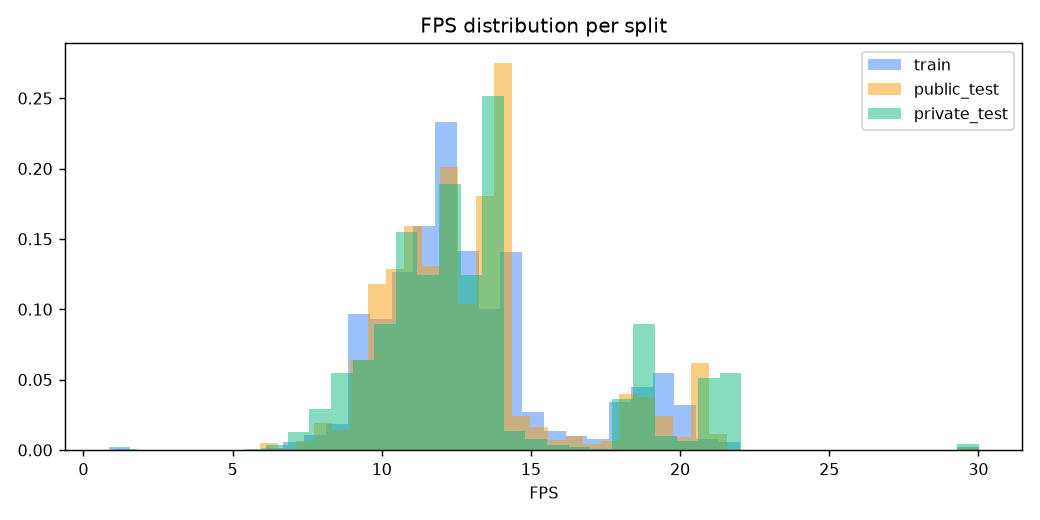
\includegraphics[width=0.85\textwidth]{fps_hist_by_split.png}
  \caption{Phân phối FPS theo từng tập.}
  \label{fig:eda_fps_hist}
\end{figure}

\paragraph{Dung lượng tệp} Dung lượng train có trung vị 80,6~KB (trung bình 85,5; từ 2,5 đến 263,8~KB). Hai tập test có phân phối lệch phải hơn hẳn: trung bình 113,6--116,3~KB, lớn nhất tới 483--488~KB (Hình~\ref{fig:eda_size_hist}); khác biệt này được phân tích ở Mục~\ref{subsec:eda_shift}.

\begin{figure}[H]
  \centering
  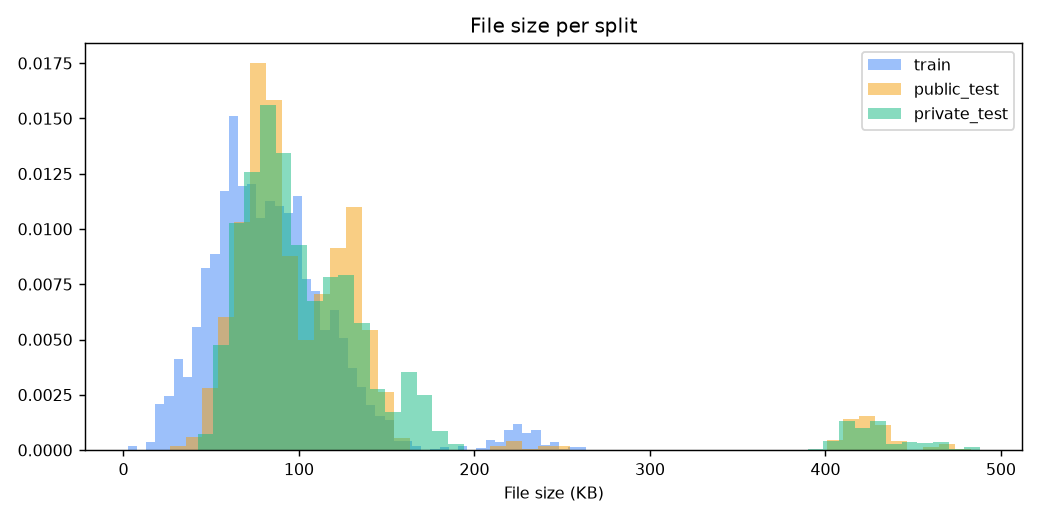
\includegraphics[width=0.85\textwidth]{filesize_hist_by_split.png}
  \caption{Phân phối dung lượng tệp (KB) theo từng tập.}
  \label{fig:eda_size_hist}
\end{figure}

\noindent\textit{Hệ quả:} (i) không cần đổi kích thước khung hình, tuy kiến trúc CRNN với \texttt{Adaptive\allowbreak AvgPool2d} vẫn đảm bảo tính tổng quát nếu gặp video khác độ phân giải; (ii) vì mọi video có ít nhất 16 khung, lấy mẫu $T=16$ khung đều nhau bằng \texttt{linspace} (\textit{Frame Downsampling}) là đủ, lặp khung (\textit{repeat padding}) chỉ giữ làm phương án dự phòng; (iii) phân phối FPS và dung lượng lệch phải với nhiều ngoại lai nên nên dùng trung vị thay vì trung bình khi mô tả.

% =====================================================================
\subsubsection{Phân tích biến mục tiêu}
\label{subsec:eda_class}

\paragraph{Script và cách thực hiện}
\begin{itemize}
  \item \textbf{Script:} \edafile{04\_target\_analysis}{01\_class\_distribution.py}.
  \item \textbf{Cách khai thác dữ liệu:} lọc các dòng của tập train trong \texttt{video\_metadata.csv}, đếm số video mỗi nhãn bằng \texttt{value\_counts()}, sau đó tính trung bình, trung vị, độ lệch chuẩn, tỷ lệ lớp lớn nhất/nhỏ nhất và số lớp có không quá 25 hoặc từ 50 video trở lên. Số video mỗi lớp sau khử trùng lặp lấy từ \texttt{class\_counts\_train\_unique\_vs\_all.csv} của bước \texttt{02\_data\_quality}.
  \item \textbf{Đầu ra:} \texttt{class\_summary.txt}, \texttt{class\_counts\_train.csv}, \texttt{class\_distribution\_all.png}, \texttt{class\_top\_bottom10.png}, \texttt{samples\_per\_class\_hist.png}.
\end{itemize}

Nhóm dùng \texttt{value\_counts()} trên cột nhãn của tập \texttt{train} để đếm số video mỗi lớp, rồi vẽ biểu đồ cho cả 100 lớp (Hình~\ref{fig:eda_class_dist}), 10 lớp nhiều nhất/ít nhất (Hình~\ref{fig:eda_top_bottom}) và histogram số video mỗi lớp (Hình~\ref{fig:eda_spc_hist}).

\begin{figure}[H]
  \centering
  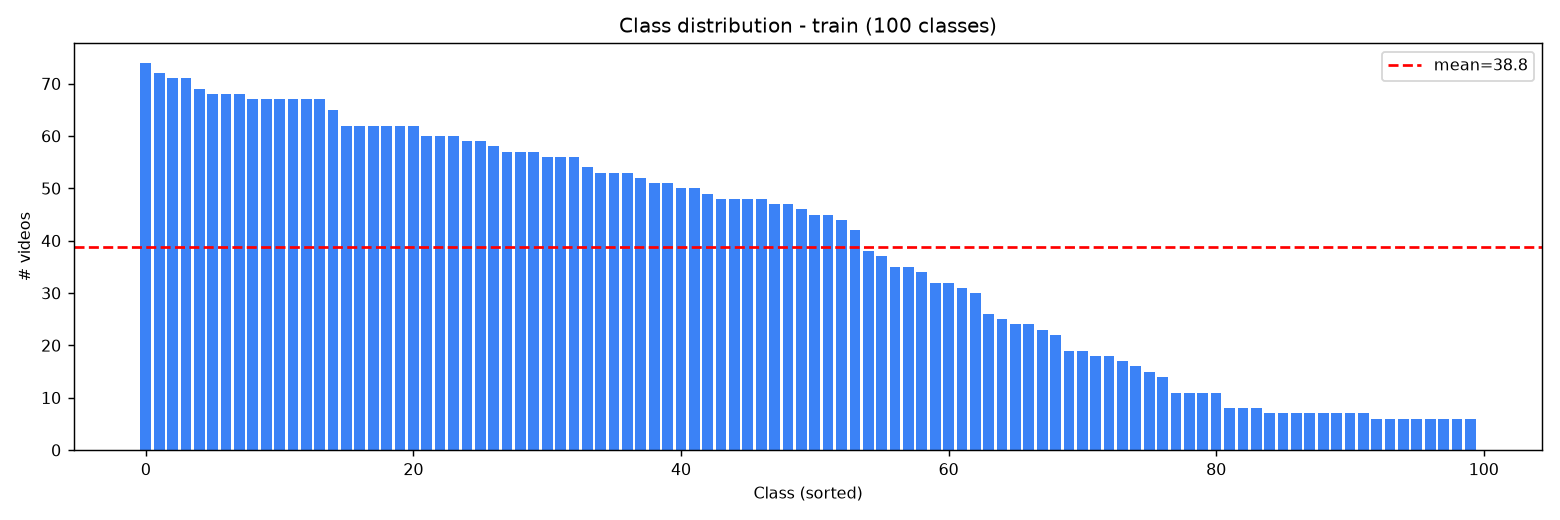
\includegraphics[width=\textwidth]{class_distribution_all.png}
  \caption{Phân phối số video theo lớp trong tập huấn luyện (100 lớp, sắp xếp giảm dần).}
  \label{fig:eda_class_dist}
\end{figure}

Tập huấn luyện gồm 3.875 video nhưng phân bố không đồng đều: trung bình 38,75 video/lớp, trung vị 45,5, độ lệch chuẩn 22,78. Lớp nhiều nhất (\textit{Trường học}) có 74 video, trong khi mười lớp chỉ có 6--7 video; tỷ lệ chênh giữa lớp lớn nhất và nhỏ nhất xấp xỉ $12{,}3$ lần (Bảng~\ref{tab:eda_top_bottom}). Có 36/100 lớp có không quá 25 video và 42/100 lớp có từ 50 video trở lên, tức phân phối có dạng hai đỉnh: nhóm lớp ``giàu'' (khoảng 45--74 video) và nhóm lớp ``nghèo'' (khoảng 6--11 video). Nhiều lớp ít mẫu thuộc nhóm từ vựng y tế -- dịch bệnh.

\begin{table}[H]
  \centering
  \caption{Mười lớp nhiều mẫu nhất và mười lớp ít mẫu nhất trong tập huấn luyện.}
  \label{tab:eda_top_bottom}
  \begin{tabular}{@{}lr@{\hspace{2.5em}}lr@{}}
    \toprule
    \multicolumn{2}{c}{\textbf{Nhiều nhất}} & \multicolumn{2}{c}{\textbf{Ít nhất}} \\
    \cmidrule(r){1-2}\cmidrule(l){3-4}
    \textbf{Lớp} & \textbf{Số video} & \textbf{Lớp} & \textbf{Số video} \\
    \midrule
    Trường học & 74 & Nhầm      & 7 \\
    Rau        & 72 & Virus     & 7 \\
    Nhà        & 71 & Bệnh nhân & 6 \\
    Áp dụng    & 71 & Cách ly   & 6 \\
    Chậm lại   & 69 & Cơ thể    & 6 \\
    Cám dỗ     & 68 & Ho        & 6 \\
    Nghe       & 68 & Phục hồi  & 6 \\
    Nói xấu    & 68 & Sốt       & 6 \\
    Biết       & 67 & Xe máy    & 6 \\
    Chạy       & 67 & Ủng hộ    & 6 \\
    \bottomrule
  \end{tabular}
\end{table}

\begin{figure}[H]
  \centering
  \begin{minipage}{0.56\textwidth}
    \centering
    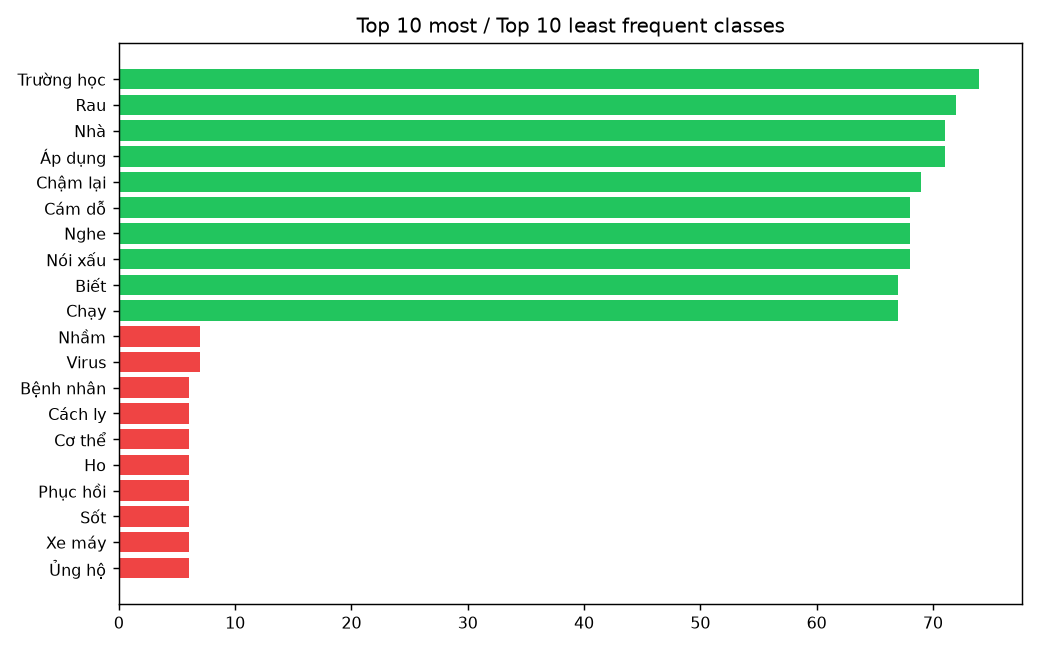
\includegraphics[width=\textwidth]{class_top_bottom10.png}
    \caption{Mười lớp nhiều nhất (xanh) và ít nhất (đỏ).}
    \label{fig:eda_top_bottom}
  \end{minipage}\hfill
  \begin{minipage}{0.42\textwidth}
    \centering
    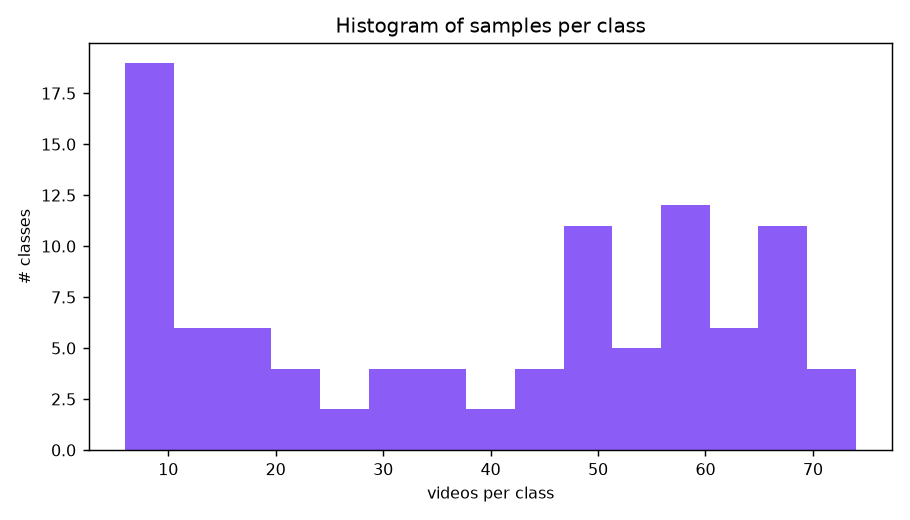
\includegraphics[width=\textwidth]{samples_per_class_hist.png}
    \caption{Histogram số video mỗi lớp.}
    \label{fig:eda_spc_hist}
  \end{minipage}
\end{figure}

Các con số trên tính trên tệp gốc, \emph{chưa} khử trùng lặp.

\noindent\textit{Hệ quả:} dữ liệu bị mất cân bằng lớp (\textit{Class Imbalance}) rõ rệt. Nếu đánh giá bằng Accuracy, mô hình có thể thiên về lớp phổ biến mà vẫn đạt điểm cao; vì vậy dùng Macro F1 (cũng là thước đo chính thức) và cần biện pháp xử lý mất cân bằng ở bước tiền xử lý/huấn luyện.

% =====================================================================
\subsubsection{Phân tích hai biến và đa biến}
\label{subsec:eda_multi}

\paragraph{Script và cách thực hiện}
\begin{itemize}
  \item \textbf{Script:} \edafile{05\_bivariate\_multivariate}{01\_correlation\_and\_label\_association.py}.
  \item \textbf{Cách khai thác dữ liệu:} ghép \texttt{video\_metadata.csv} với \texttt{video\_quality\_flags.csv} theo khoá (tập, lớp, tên tệp); bỏ các bản sao \texttt{\_N} để chỉ giữ 2.776 video duy nhất của train. Tính ma trận tương quan Pearson và Spearman (tương quan hạng, ít nhạy với ngoại lai) giữa các thuộc tính số; với từng thuộc tính, chia giá trị theo 100 lớp rồi chạy kiểm định Kruskal--Wallis (\texttt{scipy.stats.kruskal}) và tính $\eta^2 = SS_{\text{giữa lớp}}/SS_{\text{tổng}}$. Trung vị và tứ phân vị FPS của từng lớp được sắp xếp tăng dần để vẽ.
  \item \textbf{Đầu ra:} \texttt{multivariate\_summary.txt}, \texttt{corr\_heatmap.png}, \texttt{fps\_by\_class.png}, \texttt{size\_vs\_solid.png}.
\end{itemize}

Vì dữ liệu video không có đặc trưng dạng bảng, phân tích hai biến và đa biến tập trung vào mối quan hệ giữa các thuộc tính metadata với nhau và với nhãn lớp. Để tránh bản sao làm lệch kết quả, các phép tính dưới đây dùng 2.776 video duy nhất của tập train.

\paragraph{Tương quan giữa các thuộc tính} Hình~\ref{fig:eda_corr} cho thấy hệ số tương quan Pearson giữa số khung, FPS, dung lượng, tỷ lệ khung đơn sắc và độ chuyển động. (Thời lượng không đưa vào vì $\texttt{dur}=\texttt{frames}/\texttt{fps}$ nên phụ thuộc hoàn toàn vào hai biến còn lại.) Hầu hết các cặp có tương quan yếu ($|r|<0{,}35$); hai quan hệ rõ nhất là dung lượng -- tỷ lệ khung đơn sắc ($r\approx-0{,}45$; Spearman $\rho\approx-0{,}51$) và FPS -- chuyển động ($r\approx-0{,}34$; $\rho\approx-0{,}30$). Tương quan Spearman cho cùng chiều và độ lớn tương tự, nên các quan hệ này không phải do ngoại lai tạo ra. Quan hệ đầu là hợp lý: khung đơn sắc nén rất nhỏ nên video chứa nhiều khung đơn sắc có dung lượng thấp (Hình~\ref{fig:eda_size_solid}). Quan hệ sau cho thấy video có FPS thấp (clip gốc dài hơn) có độ chuyển động giữa các khung liên tiếp lớn hơn. Số khung gần như không liên quan tới các biến khác vì hầu như không đổi.

\begin{figure}[H]
  \centering
  \begin{minipage}{0.48\textwidth}
    \centering
    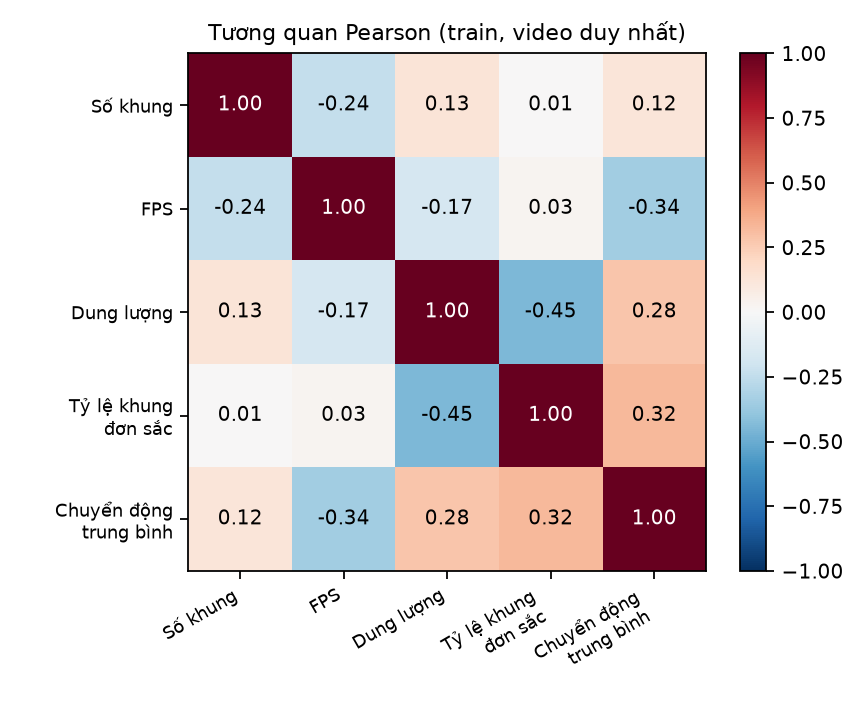
\includegraphics[width=\textwidth]{corr_heatmap.png}
    \caption{Ma trận tương quan Pearson giữa các thuộc tính (train, video duy nhất).}
    \label{fig:eda_corr}
  \end{minipage}\hfill
  \begin{minipage}{0.48\textwidth}
    \centering
    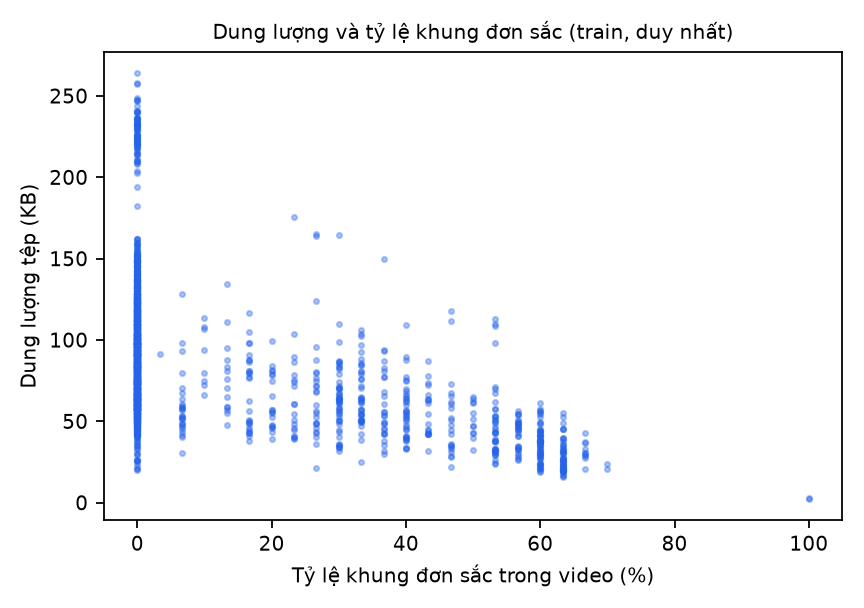
\includegraphics[width=\textwidth]{size_vs_solid.png}
    \caption{Dung lượng tệp theo tỷ lệ khung đơn sắc.}
    \label{fig:eda_size_solid}
  \end{minipage}
\end{figure}

\paragraph{Quan hệ giữa thuộc tính và nhãn lớp} Nhóm so sánh phân phối của từng thuộc tính giữa 100 lớp bằng kiểm định Kruskal--Wallis và hệ số $\eta^2$ (tỷ lệ phương sai giải thích bởi nhãn). Kết quả: FPS có $\eta^2\approx0{,}28$, dung lượng $\eta^2\approx0{,}15$, số khung $\eta^2\approx0{,}08$; cả ba đều có $p<10^{-10}$. Nói cách khác, FPS của video khác nhau rõ rệt giữa các lớp: trung vị FPS của lớp dao động từ khoảng 9,4 (\textit{Ngón tay}) đến khoảng 19,2 (\textit{Ho}), trong khi trung vị toàn tập là 12,4 (Hình~\ref{fig:eda_fps_class}). Điều này gợi ý rằng thời lượng clip gốc (và do đó FPS sau khi lấy mẫu lại) có liên hệ với từ được ký -- có thể vì các từ khác nhau có độ dài tự nhiên khác nhau -- hoặc vì cách thu thập dữ liệu theo từng lớp. Nhóm chưa xác định được nguyên nhân.

\begin{figure}[H]
  \centering
  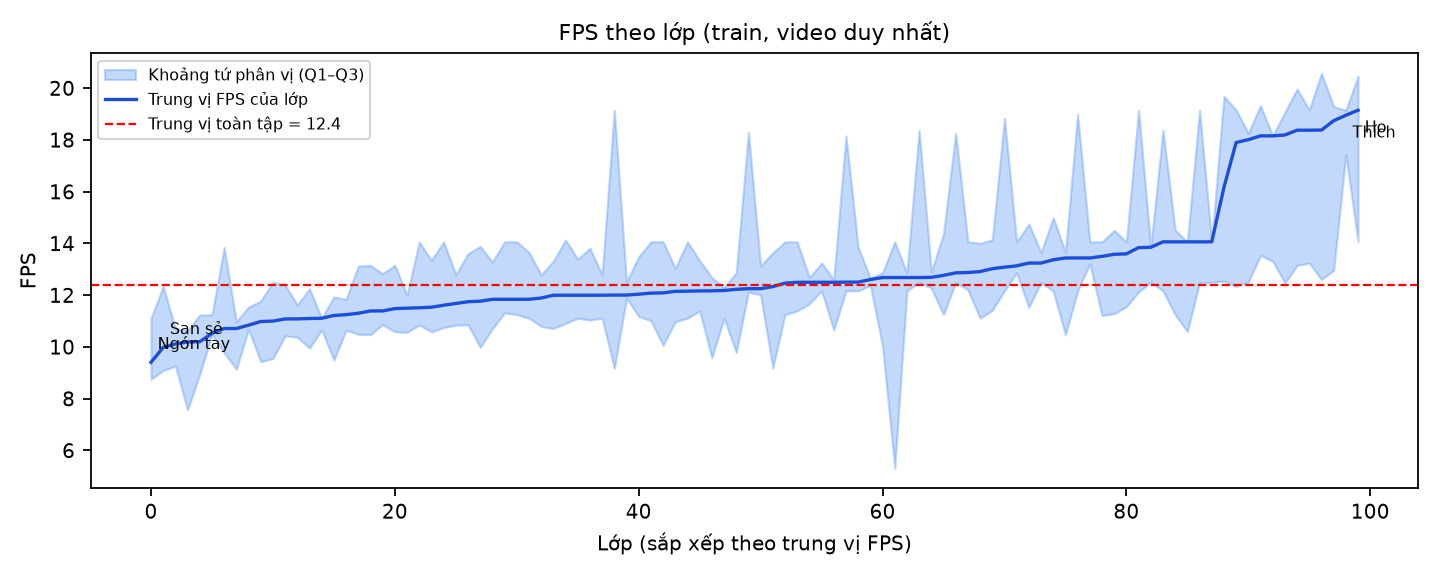
\includegraphics[width=0.95\textwidth]{fps_by_class.png}
  \caption{Trung vị và khoảng tứ phân vị của FPS theo lớp (train, video duy nhất), các lớp sắp xếp theo trung vị.}
  \label{fig:eda_fps_class}
\end{figure}

\paragraph{Khung đơn sắc theo lớp} Khung đơn sắc không phân bố đều: 78/100 lớp có ít nhất một video bị ảnh hưởng, và có lớp có tới 30--40\% video duy nhất chứa khung đơn sắc (\textit{Có thể}, \textit{Xin lỗi}, \textit{Thất lạc}, \textit{Mua}). Do đó việc loại bỏ khung đơn sắc sẽ tác động không đồng đều lên các lớp.

\noindent\textit{Hệ quả:} (i) các thuộc tính metadata phần lớn độc lập nhau nên không có cặp đặc trưng dư thừa cần loại bỏ; (ii) vì FPS và dung lượng có quan hệ thống kê với nhãn, chúng có thể trở thành ``đường tắt'' (\textit{shortcut}) mà mô hình học được thay vì học ký hiệu, nên không nên đưa FPS hoặc dung lượng làm đặc trưng đầu vào và cần theo dõi nguy cơ này khi đánh giá; (iii) cần kiểm tra lại phân phối nhãn sau khi loại khung đơn sắc.

% =====================================================================
\subsubsection{So sánh phân phối giữa các tập}
\label{subsec:eda_shift}

\paragraph{Script và cách thực hiện}
\begin{itemize}
  \item \textbf{Script:} \edafile{06\_split\_comparison}{01\_split\_shift.py}.
  \item \textbf{Cách khai thác dữ liệu:} với train chỉ giữ video duy nhất, để các bản sao không làm lệch phân phối. Với mỗi thuộc tính (\texttt{frames}, \texttt{fps}, \texttt{dur}, \texttt{size\_kb}, \texttt{motion}), script tính trung vị từng tập và chạy kiểm định Kolmogorov--Smirnov hai mẫu (\texttt{scipy.stats.ks\_2samp}) cho từng cặp tập. Thống kê $D$ là khoảng cách lớn nhất giữa hai hàm phân phối tích luỹ thực nghiệm (ECDF); $D$ càng lớn thì hai phân phối càng khác nhau. Script cũng tính tỷ lệ video có khung đơn sắc ở từng tập và số video trùng nội dung giữa các tập (theo \texttt{file\_hashes.csv}). Ngưỡng ngoại lai trên của dung lượng (167~KB, tính từ train) lấy từ bước đơn biến.
  \item \textbf{Đầu ra:} \texttt{split\_shift\_summary.txt}, \texttt{ecdf\_by\_split.png}.
\end{itemize}

Nhóm so sánh phân phối các thuộc tính giữa ba tập trên cùng trục (Bảng~\ref{tab:eda_desc}, Bảng~\ref{tab:eda_ks}, Hình~\ref{fig:eda_ecdf}) để tìm dấu hiệu khác biệt miền (\textit{Domain Shift}).

\begin{table}[H]
  \centering
  \caption{Kiểm định Kolmogorov--Smirnov hai mẫu giữa các tập (train: video duy nhất). Giá trị là thống kê $D$, trong ngoặc là $p$-value.}
  \label{tab:eda_ks}
  \small
  \begin{tabular}{@{}lccc@{}}
    \toprule
    \textbf{Thuộc tính} & \textbf{train -- public} & \textbf{train -- private} & \textbf{public -- private} \\
    \midrule
    Số khung        & 0,005 (1)                 & 0,007 (1)                 & 0,002 (1) \\
    FPS             & 0,075 ($1{,}7\cdot10^{-5}$) & 0,069 ($2{,}9\cdot10^{-6}$) & 0,094 ($1{,}7\cdot10^{-8}$) \\
    Thời lượng      & 0,075 ($1{,}7\cdot10^{-5}$) & 0,068 ($4{,}5\cdot10^{-6}$) & 0,094 ($1{,}7\cdot10^{-8}$) \\
    Dung lượng      & \textbf{0,230} ($2\cdot10^{-48}$) & \textbf{0,237} ($4\cdot10^{-70}$) & 0,059 (0,0013) \\
    Chuyển động     & 0,059 (0,0015)            & 0,079 ($4{,}8\cdot10^{-8}$) & 0,035 (0,15) \\
    \bottomrule
  \end{tabular}
\end{table}

\begin{figure}[H]
  \centering
  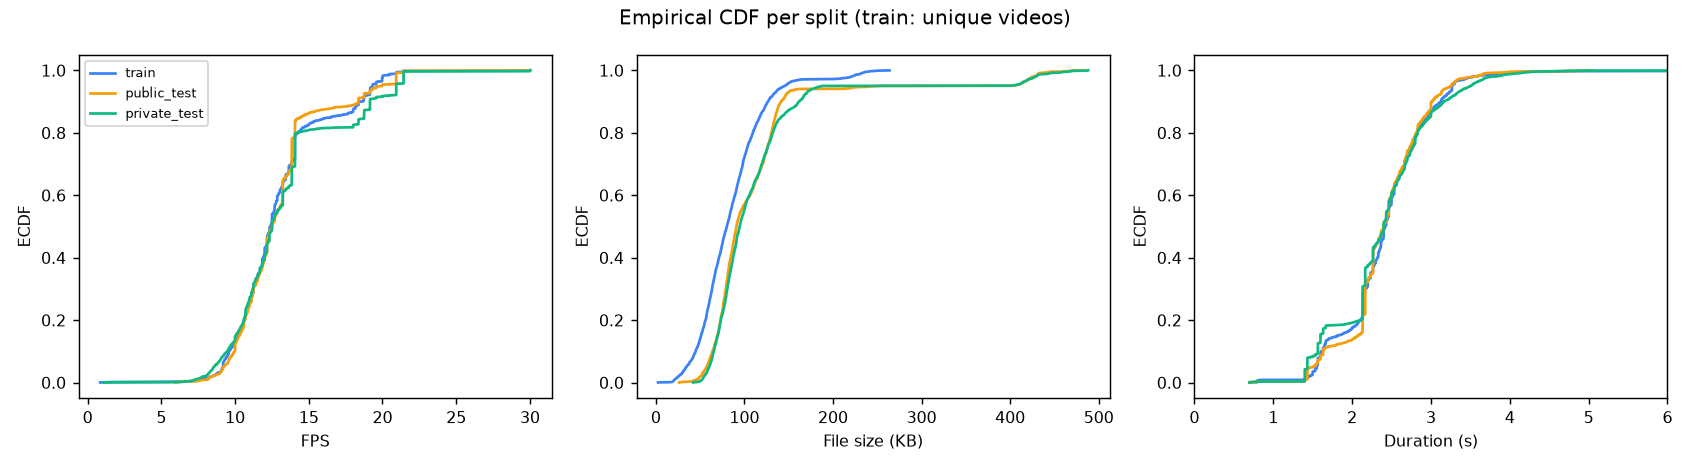
\includegraphics[width=\textwidth]{ecdf_by_split.png}
  \caption{Hàm phân phối tích luỹ thực nghiệm của FPS, dung lượng và thời lượng theo tập (train: video duy nhất). Đường dung lượng của train tách hẳn khỏi hai tập test.}
  \label{fig:eda_ecdf}
\end{figure}

Vì cỡ mẫu lớn nên mọi khác biệt dù nhỏ đều có $p$ rất bé; nhóm đánh giá chủ yếu theo độ lớn của $D$. Số khung hình giống nhau ở cả ba tập ($D<0{,}01$), độ phân giải cũng vậy. FPS, thời lượng và độ chuyển động khác biệt nhỏ ($D<0{,}1$). Riêng dung lượng khác biệt rõ giữa train và hai tập test ($D\approx0{,}23$--$0{,}24$), trong khi hai tập test gần nhau ($D\approx0{,}06$). Cụ thể:

\begin{itemize}
  \item \textbf{Dung lượng:} video test nặng hơn đáng kể (trung bình 113,6--116,3~KB so với 85,5~KB; trung vị 91,0--94,6~KB so với 80,6~KB). Tỷ lệ video vượt 167~KB (ngưỡng ngoại lai của train) là 3,1\% ở train nhưng 6,0\% ở public và 8,2\% ở private. Một phần chênh lệch có thể giải thích bởi khung đơn sắc (nén rất nhỏ) chỉ có ở train: trung vị dung lượng của video train có khung đơn sắc là 49,0~KB, còn của video train không có khung đơn sắc là 87,6~KB, gần mức của test. Tuy nhiên đuôi dài tới 488~KB ở test không xuất hiện ở train (lớn nhất 263,8~KB), cho thấy test có thể chứa các video chi tiết hoặc nhiễu hơn.
  \item \textbf{FPS:} trung vị gần như nhau (12,4 ở train, 12,5 ở hai tập test), nhưng private test có độ lệch chuẩn lớn hơn (3,69 so với 3,11 ở train) và đuôi dài hơn.
  \item \textbf{Khung đơn sắc:} khoảng 20\% video train nhưng gần như không có ở test (Bảng~\ref{tab:eda_solid}).
  \item \textbf{Người ký, nền, ánh sáng:} có thể khác giữa train và test; nhóm chưa định lượng được yếu tố này.
\end{itemize}

\noindent\textit{Hệ quả:} cần các phép tăng cường giúp mô hình bền vững với thay đổi màu sắc, độ sáng và khung cắt (\textit{ColorJitter}, \textit{Random Resized Crop}); việc loại bỏ khung đơn sắc ở train đồng thời giúp thu hẹp khoảng cách giữa phân phối train và test.

% =====================================================================
\subsubsection{Kết luận EDA và khuyến nghị cho bước tiền xử lý}
\label{subsec:eda_conclusion}

Bảng~\ref{tab:eda_reco} tổng hợp các vấn đề phát hiện được, bằng chứng và khuyến nghị cho bước tiền xử lý (Mục~\ref{sec:preprocess}) cũng như huấn luyện.

\begin{table}[H]
  \centering
  \caption{Tổng hợp vấn đề, bằng chứng và khuyến nghị cho bước tiền xử lý.}
  \label{tab:eda_reco}
  \small
  \begin{tabular}{@{}p{0.2\textwidth}p{0.36\textwidth}p{0.38\textwidth}@{}}
    \toprule
    \textbf{Vấn đề} & \textbf{Bằng chứng} & \textbf{Khuyến nghị} \\
    \midrule
    Tên lớp khác dạng Unicode & Khoá trong \texttt{label\_mapping.pkl} ở dạng NFD, thư mục lớp ở dạng NFC; 91/100 lớp không khớp nếu so nguyên văn & Chuẩn hoá NFC cả hai phía trước khi tra nhãn \\
    \addlinespace
    Video trùng lặp (\texttt{\_N}) & 1.069 tệp \texttt{\_N} giống hệt bản gốc; chỉ còn 2.776 video duy nhất & Khử trùng lặp theo MD5; chia train/validation theo ID gốc (bỏ hậu tố \texttt{\_N}) bằng \texttt{StratifiedGroupKFold} để tránh rò rỉ \\
    \addlinespace
    Mất cân bằng lớp & 6--74 video/lớp (sau khử trùng lặp: 5--51), 36/100 lớp có $\leq$25 video & Dùng Macro F1; trọng số lớp hoặc \texttt{WeightedRandomSampler}; oversample kèm tăng cường cho lớp ít mẫu; có thể dùng label smoothing \\
    \addlinespace
    Khung đơn sắc & 565/2.776 video duy nhất (20,4\%) chứa trung bình 12,2 khung đơn sắc; test gần như không có & Loại bỏ khung đơn sắc (độ lệch chuẩn điểm ảnh $<3$) \emph{trước} khi lấy mẫu $T=16$; nếu còn ít hơn 16 khung hợp lệ thì lặp khung \\
    \addlinespace
    Video rỗng & \texttt{Biết/214576}, \texttt{Khai báo/885339} (cùng 2 bản sao) đơn sắc toàn bộ & Loại khỏi tập huấn luyện \\
    \addlinespace
    Xung đột nhãn & 2 nhóm nội dung giống hệt nhưng thuộc \textit{Chậm lại} và \textit{Chào} & Xác minh nhãn đúng; nếu không xác minh được thì loại bỏ \\
    \addlinespace
    Độ dài không đồng nhất & 98,9\% video có 30 khung, tối thiểu 16 khung; thời lượng tới 35,3~s & Lấy mẫu $T=16$ khung đều bằng \texttt{linspace} \\
    \addlinespace
    FPS/dung lượng liên hệ với nhãn & $\eta^2\approx0{,}28$ (FPS), $0{,}15$ (dung lượng) giữa các lớp & Không dùng FPS, dung lượng làm đặc trưng; theo dõi nguy cơ shortcut \\
    \addlinespace
    Khác biệt miền train--test & Test nặng hơn (trung bình 114--116~KB so với 85,5~KB; KS $D\approx0{,}23$); khung đơn sắc chỉ có ở train & ColorJitter, Random Resized Crop, chuẩn hoá ImageNet; \emph{không} lật ngang \\
    \addlinespace
    Trùng train--public test & 157 video public giống hệt video train & Lưu ý khi diễn giải điểm public test \\
    \bottomrule
  \end{tabular}
\end{table}

Tóm lại, bộ dữ liệu có định dạng rất đồng nhất (100\% video $224\times224$, gần như đều 30 khung), nên khâu đọc và lấy mẫu khung đơn giản. Tuy nhiên dữ liệu huấn luyện có ba vấn đề cần xử lý trước khi huấn luyện: mất cân bằng lớp, khoảng 28\% tệp là bản sao gây nguy cơ rò rỉ dữ liệu, và khoảng 20\% video chứa khung đơn sắc vốn không xuất hiện ở dữ liệu kiểm tra. Đây là những yếu tố có thể khiến điểm validation cao hơn đáng kể so với điểm thực tế trên tập kiểm tra nếu không được xử lý.

\paragraph{Hạn chế của phân tích} FPS và thời lượng đọc từ metadata của container nên có thể không phản ánh tốc độ quay thực. Ngưỡng độ lệch chuẩn $<3$ chỉ phát hiện khung đơn sắc hoàn toàn, chưa phát hiện khung mờ hoặc chỉ có nền. Nhóm chưa định lượng sự khác biệt về người ký và bối cảnh giữa train và test, chưa xác định được nguyên nhân FPS liên hệ với nhãn, và chưa xác định được nhãn đúng cho các video xung đột.
]
% Cấu trúc theo khung EDA chuẩn:
%   3.1.1 Mục tiêu và tổng quan dữ liệu
%   3.1.2 Cấu trúc dữ liệu
%   3.1.3 Chất lượng dữ liệu
%   3.1.4 Phân tích đơn biến
%   3.1.5 Phân tích biến mục tiêu
%   3.1.6 Phân tích hai biến và đa biến
%   3.1.7 So sánh phân phối giữa các tập
%   3.1.8 Kết luận và khuyến nghị
% Gói cần: graphicx, booktabs, float, caption, amsmath
% =====================================================================

\subsection{Phân tích dữ liệu (EDA)}
\label{sec:eda}

% \edafile{thư mục}{tệp}: in đường dẫn script, cho phép xuống dòng sau dấu /
\newcommand{\edafile}[2]{\texttt{#1/}\allowbreak\texttt{#2}}
% Cho phép xuống dòng sau dấu gạch dưới trong tên tệp dài (vd. class\_counts\_train\_unique\_vs\_all.csv)
\let\edaOrigUS\_
\renewcommand{\_}{\edaOrigUS\allowbreak}
\sloppy

Mục này trình bày kết quả phân tích khám phá dữ liệu (\textit{Exploratory Data Analysis -- EDA}) trên bộ dữ liệu video ngôn ngữ ký hiệu. EDA chỉ nhằm \emph{quan sát} xu hướng, phân phối và chất lượng dữ liệu. Nhóm sử dụng Python làm công cụ để thực hiện EDA (\texttt{os}, \texttt{pickle}, \texttt{pandas}, \texttt{OpenCV}, \texttt{numpy}, \texttt{hashlib}, \texttt{matplotlib}).

Phần phân tích được tổ chức theo trình tự quy trình EDA: tổng quan và cấu trúc dữ liệu (Mục~\ref{subsec:eda_overview}--\ref{subsec:eda_structure}), chất lượng dữ liệu (Mục~\ref{subsec:eda_quality}), phân tích đơn biến (Mục~\ref{subsec:eda_uni}), phân tích biến mục tiêu (Mục~\ref{subsec:eda_class}), phân tích hai biến và đa biến (Mục~\ref{subsec:eda_multi}), so sánh giữa các tập (Mục~\ref{subsec:eda_shift}) và cuối cùng là kết luận kèm khuyến nghị (Mục~\ref{subsec:eda_conclusion}).

\begin{table}[H]
  \centering
  \caption{Các script EDA, thứ tự chạy và mục sử dụng kết quả.}
  \label{tab:eda_scripts}
  \small
  \begin{tabular}{@{}p{0.17\textwidth}p{0.26\textwidth}p{0.27\textwidth}p{0.18\textwidth}@{}}
    \toprule
    \textbf{Bước (thư mục)} & \textbf{Script -- câu hỏi} & \textbf{Kết quả chính} & \textbf{Dùng ở} \\
    \midrule
    \texttt{01\_overview} & \texttt{01\_scan\_metadata.py} -- dữ liệu gồm những gì? & \texttt{video\_metadata.csv} & 3.1.1 \\
      & \texttt{02\_dataset\_structure.py} -- chia tập, định dạng, tệp nhãn & \texttt{structure\_summary.txt} \newline \texttt{split\_sizes.png} & 3.1.2 \\
    \midrule
    \texttt{02\_data\_quality} & \texttt{01\_integrity\_missing.py} -- giá trị thiếu, tệp lỗi & \texttt{integrity\_summary.txt} & 3.1.3 \\
      & \texttt{02\_duplicates.py} -- trùng lặp, xung đột nhãn, trùng giữa các tập & \texttt{file\_hashes.csv} \newline \texttt{dups\_summary.txt} \newline \texttt{dedup\_summary.txt} \newline \texttt{class\_counts\_train\_unique\_vs\_all.csv} & 3.1.3, 3.1.5 \\
      & \texttt{03\_frame\_scan.py} -- quét nội dung từng khung & \texttt{video\_quality\_flags.csv} & 3.1.3, 3.1.6, 3.1.7 \\
      & \texttt{04\_frame\_quality\_summary.py} -- tổng hợp khung đơn sắc & \texttt{solid\_frame\_summary.txt} \newline \texttt{class\_solid\_frame\_ratio.csv} & 3.1.3, 3.1.6 \\
    \midrule
    \texttt{03\_univariate} & \texttt{01\_numeric\_attributes.py} -- phân phối, ngoại lai & \texttt{desc\_by\_split.csv} \newline \texttt{univariate\_summary.txt} \newline 3 histogram & 3.1.3, 3.1.4 \\
    \midrule
    \texttt{04\_target\_analysis} & \texttt{01\_class\_distribution.py} -- phân phối nhãn & \texttt{class\_summary.txt} \newline \texttt{class\_counts\_train.csv} \newline 3 hình & 3.1.5 \\
    \midrule
    \texttt{05\_bivariate\_multivariate} & \texttt{01\_correlation\_and\_label\_association.py} & \texttt{multivariate\_summary.txt} \newline 3 hình & 3.1.6 \\
    \midrule
    \texttt{06\_split\_comparison} & \texttt{01\_split\_shift.py} -- khác biệt phân phối giữa các tập & \texttt{split\_shift\_summary.txt} \newline \texttt{ecdf\_by\_split.png} & 3.1.7 \\
    \midrule
    \texttt{07\_visual\_inspection} & \texttt{01\_sample\_frames.py} -- khung hình mẫu & 2 lưới khung hình & 3.1.2 \\
      & \texttt{02\_flagged\_videos.py} -- xem lại video bị đánh dấu & \texttt{flagged\_videos\_info.txt} \newline 2 hình & 3.1.3 \\
    \bottomrule
  \end{tabular}
\end{table}

% =====================================================================
\subsubsection{Mục tiêu và tổng quan dữ liệu}
\label{subsec:eda_overview}

\paragraph{Bài toán và thước đo} Bài toán là phân loại video ngôn ngữ ký hiệu (\textit{Sign Language Video Classification}) thành $N=100$ lớp từ vựng tiếng Việt. Đầu vào là một video ghi cử chỉ của một người, được tiền xử lý thành chuỗi $T=16$ khung hình RGB; đầu ra là nhãn dự đoán. Thước đo chính thức là Macro F1-Score. Biến mục tiêu là nhãn lớp (biến phân loại, 100 giá trị), còn các thuộc tính mô tả video (số khung hình, FPS, dung lượng\ldots) chỉ đóng vai trò thông tin phụ trợ cho phân tích.

\paragraph{Nguồn dữ liệu} Bộ dữ liệu là đề chính thức của cuộc thi \textit{Olympic Trí tuệ Nhân tạo Sinh viên 2025 -- Vòng Sơ loại} do Khoa Trí tuệ Nhân tạo, Học viện Công nghệ Bưu chính Viễn thông (PTIT) tổ chức. Các lớp thuộc nhiều nhóm chủ đề: y tế -- dịch bệnh (\textit{Bệnh viện}, \textit{Cách ly}, \textit{Khẩu trang}, \textit{Virus}, \textit{Sốt}, \textit{Ho}\ldots), cảm xúc (\textit{Lo lắng}, \textit{Xúc động}, \textit{Thương}, \textit{Ghét}\ldots), hành động thường ngày (\textit{Ăn}, \textit{Uống}, \textit{Chạy}, \textit{Đi}, \textit{Mua}\ldots), thời gian -- vị trí (\textit{Ban ngày}, \textit{Trưa}, \textit{Hôm nay}, \textit{Phía sau}, \textit{Rẽ trái}\ldots) và phương tiện (\textit{Ô tô}, \textit{Xe máy}, \textit{Xe đạp}).

\paragraph{Từ điển dữ liệu} Vì dữ liệu là video nên không có bảng thuộc tính sẵn. Nhóm duyệt cây thư mục, mở từng video bằng \texttt{cv2.VideoCapture} và gom thông tin vào một bảng metadata duy nhất (\texttt{01\_overview/video\_metadata.csv}, 8.364 dòng). Mã băm MD5 được lưu ở \texttt{02\_data\_quality/file\_hashes.csv}, còn các thuộc tính suy ra từ nội dung khung hình (khung đơn sắc, chuyển động) được lưu ở \texttt{02\_data\_quality/video\_quality\_flags.csv}. Ba bảng có chung khoá (tập, lớp, tên tệp). Bảng~\ref{tab:eda_dict} liệt kê ý nghĩa từng thuộc tính; mọi thống kê phía sau chỉ là phép ghép và \texttt{groupby} trên ba bảng này.

\begin{table}[H]
  \centering
  \caption{Từ điển các thuộc tính dùng trong phân tích.}
  \label{tab:eda_dict}
  \small
  \begin{tabular}{@{}p{0.22\textwidth}p{0.17\textwidth}p{0.5\textwidth}@{}}
    \toprule
    \textbf{Thuộc tính} & \textbf{Kiểu} & \textbf{Ý nghĩa / cách tính} \\
    \midrule
    \texttt{split}        & phân loại & Tập chứa video: \texttt{train}, \texttt{public\_test}, \texttt{private\_test} \\
    \texttt{cls}          & phân loại & Nhãn lớp, lấy từ tên thư mục con của \texttt{train} (không có ở hai tập test) \\
    \texttt{file}         & chuỗi     & Tên tệp \texttt{.mp4}; hậu tố \texttt{\_N} biểu thị bản sao \\
    \texttt{frames}       & số nguyên & Số khung hình (\texttt{CAP\_\allowbreak PROP\_\allowbreak FRAME\_\allowbreak COUNT}) \\
    \texttt{fps}          & số thực   & Tốc độ khung hình ghi trong container \\
    \texttt{w}, \texttt{h}& số nguyên & Chiều rộng, chiều cao khung hình (pixel) \\
    \texttt{dur}          & số thực   & Thời lượng (giây) $=\texttt{frames}/\texttt{fps}$ \\
    \texttt{size\_kb}     & số thực   & Dung lượng tệp (KB) \\
    \texttt{md5}          & chuỗi     & Mã băm nội dung tệp, dùng phát hiện video trùng (lưu trong \texttt{file\_hashes.csv}) \\
    \texttt{solid\_ratio} & số thực   & Tỷ lệ khung đơn sắc trong video (khung có độ lệch chuẩn điểm ảnh $<3$) \\
    \texttt{motion}       & số thực   & Độ chuyển động trung bình $\overline{|f_t-f_{t-1}|}$ giữa các khung liên tiếp (ảnh xám) \\
    \bottomrule
  \end{tabular}
\end{table}

% =====================================================================
\subsubsection{Cấu trúc dữ liệu}
\label{subsec:eda_structure}

\paragraph{Quy mô và cách chia} Sau khi giải nén \texttt{dataset.zip} (khoảng 864~MB), dữ liệu gồm ba tập video và một tệp ánh xạ nhãn (Bảng~\ref{tab:eda_splits}, Hình~\ref{fig:eda_split_sizes}). Tệp \texttt{label\_mapping.pkl} là một \texttt{dict[str, int]} chứa đúng 100 lớp, đánh chỉ số 0--99 theo thứ tự bảng chữ cái tiếng Việt (\textit{An ủi}~$=0$, \textit{Áp dụng}~$=1$, \textit{Ăn}~$=2$, \ldots, \textit{Đồng ý}~$=99$). Khi đối chiếu với tên thư mục lớp, nhóm phát hiện hai bên dùng \emph{hai dạng chuẩn hoá Unicode khác nhau}: khoá trong \texttt{label\_mapping.pkl} ở dạng NFD (dấu tách rời khỏi chữ cái), còn tên thư mục ở dạng NFC (dấu dựng sẵn). Vì vậy 91/100 tên lớp (mọi lớp có dấu) không khớp nếu so nguyên văn, dù hiển thị giống hệt nhau; sau khi chuẩn hoá cả hai về NFC thì 100 lớp khớp hoàn toàn và chỉ số liên tục 0--99 không trùng.

\begin{table}[H]
  \centering
  \caption{Cấu trúc và quy mô các tập dữ liệu.}
  \label{tab:eda_splits}
  \begin{tabular}{@{}lp{0.42\textwidth}rr@{}}
    \toprule
    \textbf{Thành phần} & \textbf{Nội dung} & \textbf{Số video} & \textbf{Dung lượng} \\
    \midrule
    \texttt{train/}         & 100 thư mục con, mỗi thư mục là một lớp (có nhãn) & 3.875 & 323~MB \\
    \texttt{public\_test/}  & Video không nhãn, dùng cho bảng xếp hạng công khai & 1.630 & 181~MB \\
    \texttt{private\_test/} & Video không nhãn, dùng cho xếp hạng cuối cùng      & 2.859 & 325~MB \\
    \texttt{label\_mapping.pkl} & \texttt{dict[str, int]}: tên lớp (Unicode NFD) $\rightarrow$ chỉ số 0--99 & -- & -- \\
    \midrule
    \textbf{Tổng} & & \textbf{8.364} & $\approx$\textbf{829~MB} \\
    \bottomrule
  \end{tabular}
\end{table}

\begin{figure}[H]
  \centering
  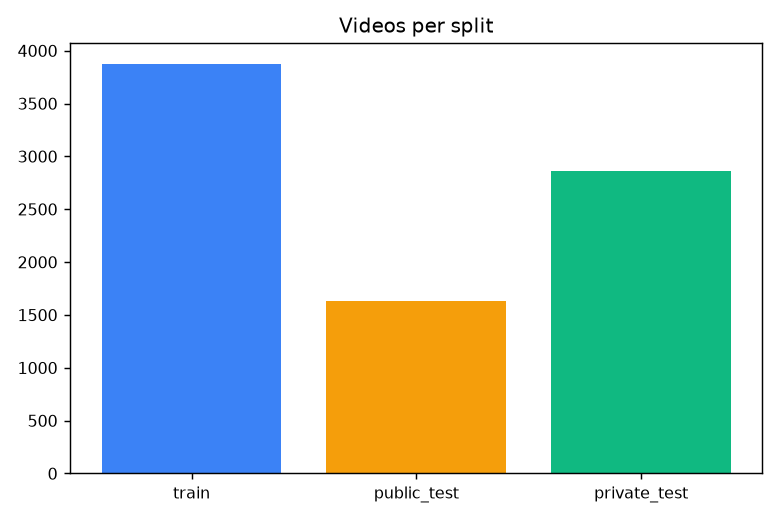
\includegraphics[width=0.6\textwidth]{split_sizes.png}
  \caption{Số lượng video trong ba tập \texttt{train}, \texttt{public\_test} và \texttt{private\_test}.}
  \label{fig:eda_split_sizes}
\end{figure}

\paragraph{Định dạng video} Toàn bộ 8.364 tệp đều là \texttt{.mp4} và đọc được; không có video nào có 0 khung hình. Độ phân giải đồng nhất tuyệt đối: 100\% video ở cả ba tập đều là $224\times224$ (Bảng~\ref{tab:eda_res}). Số khung hình gần như cố định ở mức 30 (chi tiết ở Mục~\ref{subsec:eda_uni}).

\begin{table}[H]
  \centering
  \caption{Thống kê độ phân giải video.}
  \label{tab:eda_res}
  \begin{tabular}{@{}lrrr@{}}
    \toprule
    \textbf{Tập} & \textbf{Độ phân giải} & \textbf{Số video} & \textbf{Tỷ lệ} \\
    \midrule
    train         & $224\times224$ & 3.875 & 100\% \\
    public\_test  & $224\times224$ & 1.630 & 100\% \\
    private\_test & $224\times224$ & 2.859 & 100\% \\
    \bottomrule
  \end{tabular}
\end{table}

\paragraph{Quan sát trực quan} Để kiểm chứng bằng mắt, nhóm trích 6--8 khung hình phân bố đều trong video (\texttt{cap.set(cv2.CAP\_\allowbreak PROP\_\allowbreak POS\_\allowbreak FRAMES, i)} với $i$ lấy từ \texttt{np.linspace}) và ghép thành lưới ảnh cho một số lớp (Hình~\ref{fig:eda_samples}). Các video được quay chính diện, người ký ngồi hoặc đứng giữa khung hình, thấy rõ phần thân trên, hai tay và khuôn mặt; nền chủ yếu là tường trơn với ánh sáng trong nhà. Sự đa dạng nằm ở người ký (giới tính, trang phục, kính), màu nền (be, xanh nhạt, trắng) và vị trí tay lúc bắt đầu. Ký hiệu thường chỉ chiếm một phần thời lượng: các khung đầu và cuối thường là tư thế nghỉ. Ở một số video xuất hiện các khung \emph{đơn sắc hoàn toàn} (hàng \textit{Phỏng vấn}, \textit{Uống}); hiện tượng này được định lượng ở Mục~\ref{subsec:eda_quality}.

\begin{figure}[H]
  \centering
  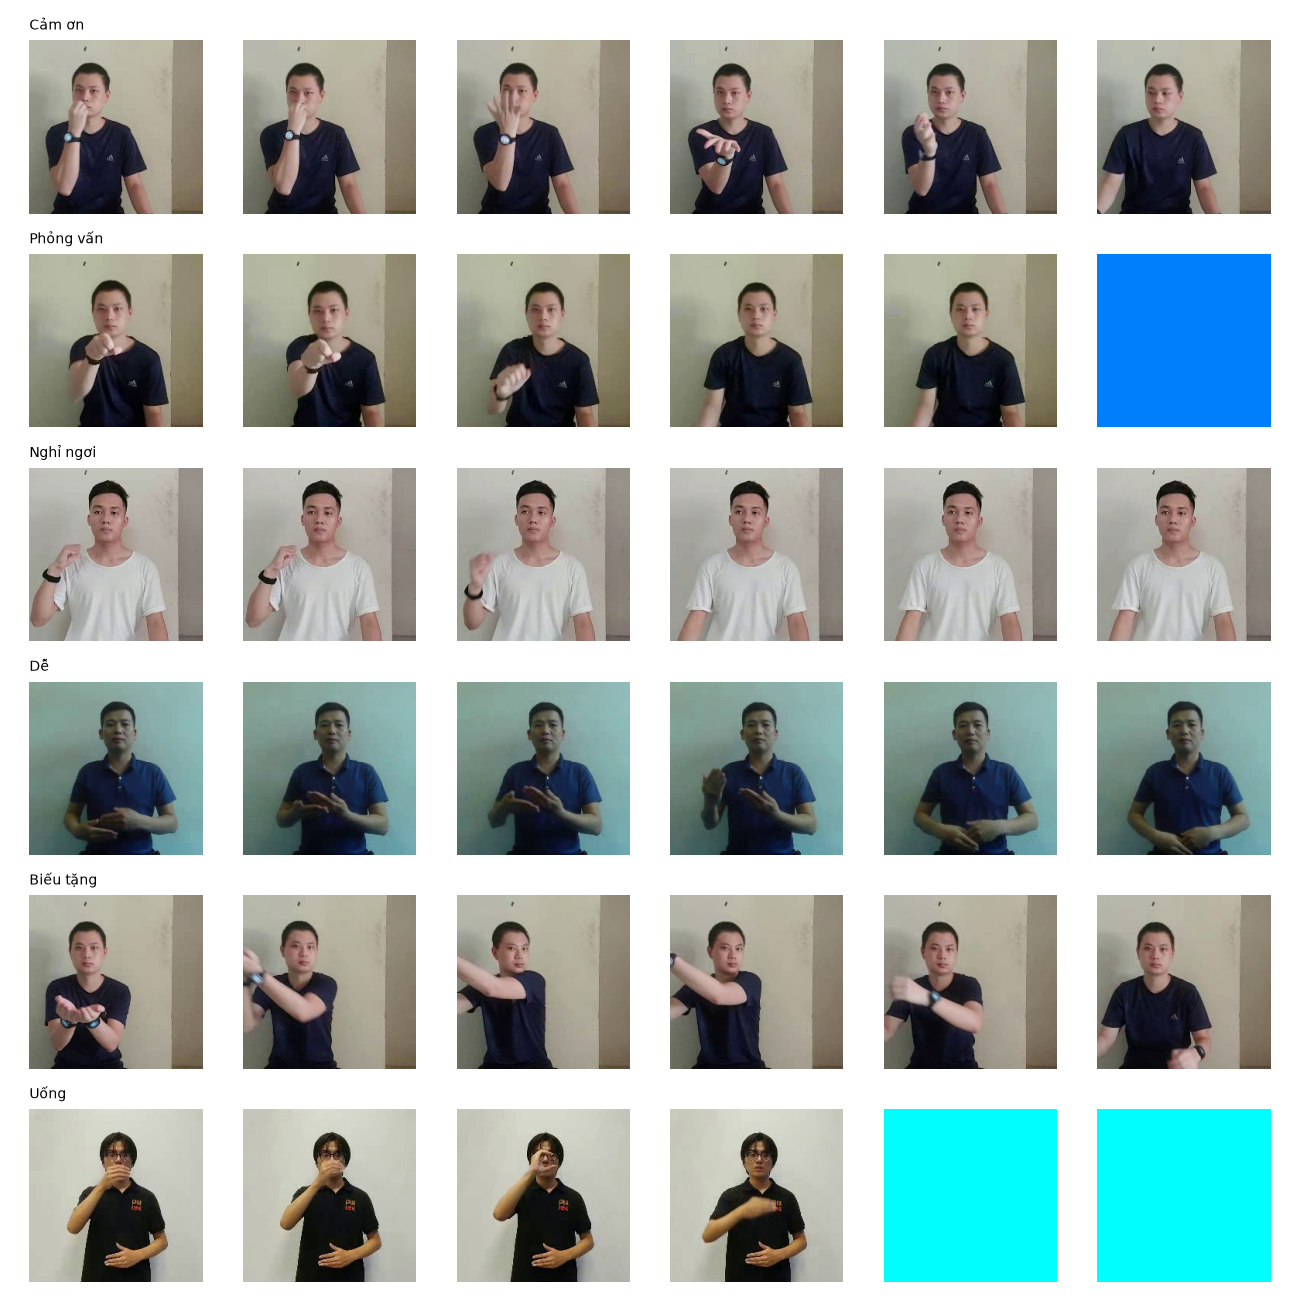
\includegraphics[width=0.85\textwidth]{sample_frames_6classes.png}
  \caption{Khung hình mẫu (lấy đều theo thời gian) của sáu lớp. Hàng \textit{Phỏng vấn} và \textit{Uống} có các khung đơn sắc ở cuối video.}
  \label{fig:eda_samples}
\end{figure}

\noindent\textit{Hệ quả:} khi gán nhãn số cho video phải chuẩn hoá tên lớp bằng \texttt{unicodedata.normalize(\textquotesingle NFC\textquotesingle, ...)} trước khi tra \texttt{label\_mapping.pkl}, nếu không phần lớn video sẽ không tìm được nhãn. Chỉ có tập \texttt{train} mang nhãn nên tập kiểm định (\textit{validation}) phải tách ra từ chính tập này; việc tách cần tính đến trùng lặp (Mục~\ref{subsec:eda_quality}). Thông tin phân biệt nằm ở hình dạng và chuyển động của bàn tay, khẩu hình và tư thế, nên các phép tăng cường không được làm đổi ngữ nghĩa không gian; đặc biệt \emph{không} dùng lật ngang (\textit{Horizontal Flip}) vì có thể đổi nghĩa tay trái/phải.

% =====================================================================
\subsubsection{Chất lượng dữ liệu}
\label{subsec:eda_quality}

\paragraph{Script và cách thực hiện}
\begin{itemize}
  \item \textbf{Script:} bốn script trong \texttt{02\_data\_quality/}, chạy theo thứ tự: \edafile{02\_data\_quality}{01\_integrity\_missing.py}, \edafile{02\_data\_quality}{02\_duplicates.py}, \edafile{02\_data\_quality}{03\_frame\_scan.py}, \edafile{02\_data\_quality}{04\_frame\_quality\_summary.py}. Kiểm tra bằng mắt dùng \edafile{07\_visual\_inspection}{02\_flagged\_videos.py}.
  \item \textbf{Cách khai thác dữ liệu:} 
  
  (i) \emph{Giá trị thiếu và lỗi đọc:} \texttt{01\_integrity\_missing.py} đếm ô trống (\texttt{isna}) theo cột và theo tập, đếm video có 0 khung, FPS hoặc kích thước bằng 0, rồi liệt kê các tệp có giá trị phi lý theo ngưỡng tuyệt đối (dưới 10~KB, dưới 16 khung, FPS dưới 5). 
  
  (ii) \emph{Trùng lặp:} \texttt{02\_duplicates.py} đọc toàn bộ byte của từng tệp, tính \texttt{hashlib.md5} một lần và lưu vào \texttt{file\_hashes.csv}; hai tệp cùng mã băm là cùng nội dung. Gom nhóm theo mã băm để đếm bản sao, tìm nhóm có nhiều hơn một nhãn (xung đột nhãn), lấy giao các tập mã băm giữa train, public test, private test, rồi giữ một tệp cho mỗi mã băm và đếm lại số video mỗi lớp. 
  
  (iii) \emph{Khung đơn sắc:} \texttt{03\_frame\_scan.py} giải mã \emph{từng} khung bằng \texttt{cap.read()}, tính độ lệch chuẩn điểm ảnh của từng kênh màu và coi khung là đơn sắc khi giá trị lớn nhất nhỏ hơn 3; đồng thời đếm số khung đơn sắc liên tiếp ở đầu video và tính độ chuyển động là trung bình $|f_t-f_{t-1}|$ trên ảnh xám. \texttt{04\_frame\_quality\_summary.py} đối chiếu số khung đọc được với metadata, bỏ các bản sao \texttt{\_N}, phân loại vị trí khung đơn sắc (đầu, cuối, giữa, toàn bộ) và mô phỏng việc lấy $T=16$ khung bằng \texttt{np.linspace} để đếm số khung đơn sắc bị lấy trúng. 
  
  (iv) \emph{Kiểm tra bằng mắt:} \texttt{02\_flagged\_videos.py} \emph{tự chọn} video cần xem từ kết quả hai bước trên, không dùng danh sách chọn tay. Tiêu chí chọn gồm: 6 video có tỷ lệ khung đơn sắc cao nhất trong số các video có từ 50\% khung đơn sắc trở lên; mọi video thuộc nhóm MD5 nằm ở hơn một lớp; một ví dụ cho mỗi dạng xuất hiện khung đơn sắc. Ngoại lai theo quy tắc Tukey được tính ở bước đơn biến (Mục~\ref{subsec:eda_uni}).
  \item \textbf{Đầu ra:} \texttt{integrity\_summary.txt}, \texttt{file\_hashes.csv}, \texttt{dups\_summary.txt}, \texttt{dedup\_summary.txt}, \texttt{class\_counts\_train\_unique\_vs\_all.csv}, \texttt{video\_quality\_flags.csv}, \texttt{solid\_frame\_summary.txt}, \texttt{class\_solid\_frame\_ratio.csv}; ở bước kiểm tra bằng mắt là \texttt{flagged\_videos\_info.txt}, \texttt{flagged\_videos\_check.png}, \texttt{solid\_frame\_patterns.png}.
\end{itemize}

Nhóm kiểm tra chất lượng dữ liệu theo các khía cạnh: giá trị thiếu, bản ghi trùng lặp, khung hình đơn sắc/video rỗng, giá trị ngoại lai, nhiễu nhãn và trùng lặp giữa các tập. Bảng~\ref{tab:eda_quality} tóm tắt các vấn đề phát hiện được.

\begin{table}[H]
  \centering
  \caption{Tóm tắt các vấn đề chất lượng dữ liệu.}
  \label{tab:eda_quality}
  \small
  \begin{tabular}{@{}p{0.26\textwidth}p{0.36\textwidth}p{0.30\textwidth}@{}}
    \toprule
    \textbf{Vấn đề} & \textbf{Số lượng} & \textbf{Ví dụ} \\
    \midrule
    Bản sao hậu tố \texttt{\_N} trong train & 1.069 tệp giống hệt bản gốc; còn 2.776 video duy nhất & \texttt{127824.mp4}, \texttt{127824\_1.mp4}, \texttt{127824\_2.mp4} \\
    Video có khung đơn sắc (train) & 758/3.875 tệp; 565/2.776 video duy nhất (20,4\%), ở 78/100 lớp & \texttt{Thất lạc/708519}, \texttt{Bộ y tế/523389} \\
    Video rỗng hoàn toàn & 2 video gốc (4 tệp kể cả bản sao) & \texttt{Biết/214576}, \texttt{Khai báo/885339} \\
    Nhiễu nhãn (cùng nội dung, khác lớp) & 2 nhóm nội dung, 5 tệp & \textit{Chậm lại} $\leftrightarrow$ \textit{Chào} \\
    Trùng train $\rightarrow$ public test & 157 video public giống hệt video train & -- \\
    Trùng public $\leftrightarrow$ private & 896 video & -- \\
    \bottomrule
  \end{tabular}
\end{table}

\paragraph{Giá trị thiếu và lỗi đọc} Bảng metadata không có giá trị thiếu ở bất kỳ thuộc tính nào (nhãn \texttt{cls} chỉ trống ở hai tập test vì các tập này vốn không có nhãn). Mọi video đều mở và giải mã được, và ở cả 8.364 video, số khung giải mã thực tế khớp với số khung ghi trong metadata. Như vậy không có vấn đề về tệp hỏng hay nhãn bị thiếu ở tập train.

\paragraph{Trùng lặp trong tập train} Nhóm tính mã băm MD5 nội dung từng tệp (\texttt{hashlib.md5}) rồi gom nhóm theo mã băm. Có 1.069/3.875 tệp mang hậu tố \texttt{\_1}, \texttt{\_2}, \texttt{\_3}\ldots{} So sánh từng cặp cho thấy cả 1.069 tệp này đều có bản gốc tồn tại, cùng lớp và \emph{giống hệt bản gốc từng byte} (cùng số khung, FPS, dung lượng): đây là bản sao, không phải biến thể tăng cường. Có 176 video gốc có 1 bản sao, 169 video có 2 và 185 video có 3. Tính cả các bản sao khác, tập train có 1.099 tệp dư thừa và chỉ còn \textbf{2.776 video duy nhất}. Các bản sao tập trung ở những lớp vốn đã nhiều mẫu (\textit{Chậm lại} và \textit{Trường học} cùng thêm 25 tệp, \textit{Rau} và \textit{Nhìn} thêm 23, \textit{Khóc} thêm 22\ldots), nên sau khi khử trùng lặp số video mỗi lớp còn từ 5 đến 51 (trung bình 27,8; tỷ lệ chênh $\approx$10,2 lần). Bảng trước/sau khử trùng lặp của từng lớp lưu ở \texttt{class\_counts\_train\_unique\_vs\_all.csv}. Hệ quả là nguy cơ rò rỉ dữ liệu (\textit{Data Leakage}): nếu chia train/validation ngẫu nhiên theo từng tệp, các bản sao của cùng một video rơi vào cả hai phần, làm điểm validation bị thổi phồng.

\paragraph{Khung hình đơn sắc và video rỗng} Nhóm đọc \emph{toàn bộ} khung hình của 8.364 video và tính độ lệch chuẩn giá trị điểm ảnh trên từng kênh màu; khung có độ lệch chuẩn lớn nhất giữa ba kênh nhỏ hơn 3 được coi là \emph{khung đơn sắc}. Kết quả tổng hợp ở Bảng~\ref{tab:eda_solid}.

\begin{table}[H]
  \centering
  \caption{Số video chứa khung hình đơn sắc theo từng tập.}
  \label{tab:eda_solid}
  \begin{tabular}{@{}lrrrr@{}}
    \toprule
    \textbf{Tập} & \textbf{Tổng video} & \textbf{Có $\geq$1 khung đơn sắc} & \textbf{Đơn sắc toàn bộ} & \textbf{Tỷ lệ} \\
    \midrule
    train (tất cả tệp)        & 3.875 & 758 & 4 & 19,6\% \\
    train (video duy nhất)    & 2.776 & 565 & 2 & 20,4\% \\
    public\_test              & 1.630 & 1   & 0 & 0,06\% \\
    private\_test             & 2.859 & 1   & 0 & 0,03\% \\
    \bottomrule
  \end{tabular}
\end{table}

Đây là phát hiện đáng chú ý nhất của EDA. Khoảng một phần năm số video duy nhất trong train (565/2.776, thuộc 78/100 lớp) chứa khung đơn sắc, và số khung này không nhỏ: trung bình 12,2 khung trên khoảng 30 khung mỗi video (trung vị 12, nhiều nhất 23). Các khung có màu thuần (đỏ, xanh lục, xanh lam, xanh lục lam, tím, vàng, trắng, đen, xám) và xuất hiện theo các dạng: chỉ ở đầu video (231 video), chỉ ở cuối (161), cả đầu và cuối (116), xen ở giữa (55) hoặc toàn bộ video (2) (Hình~\ref{fig:eda_solid_examples}). Lớp có tỷ lệ video bị ảnh hưởng cao nhất là \textit{Có thể} (6/15 video duy nhất), \textit{Xin lỗi} (5/14) và \textit{Thất lạc} (7/20) (chi tiết ở \texttt{class\_solid\_frame\_ratio.csv}).

\begin{figure}[H]
  \centering
  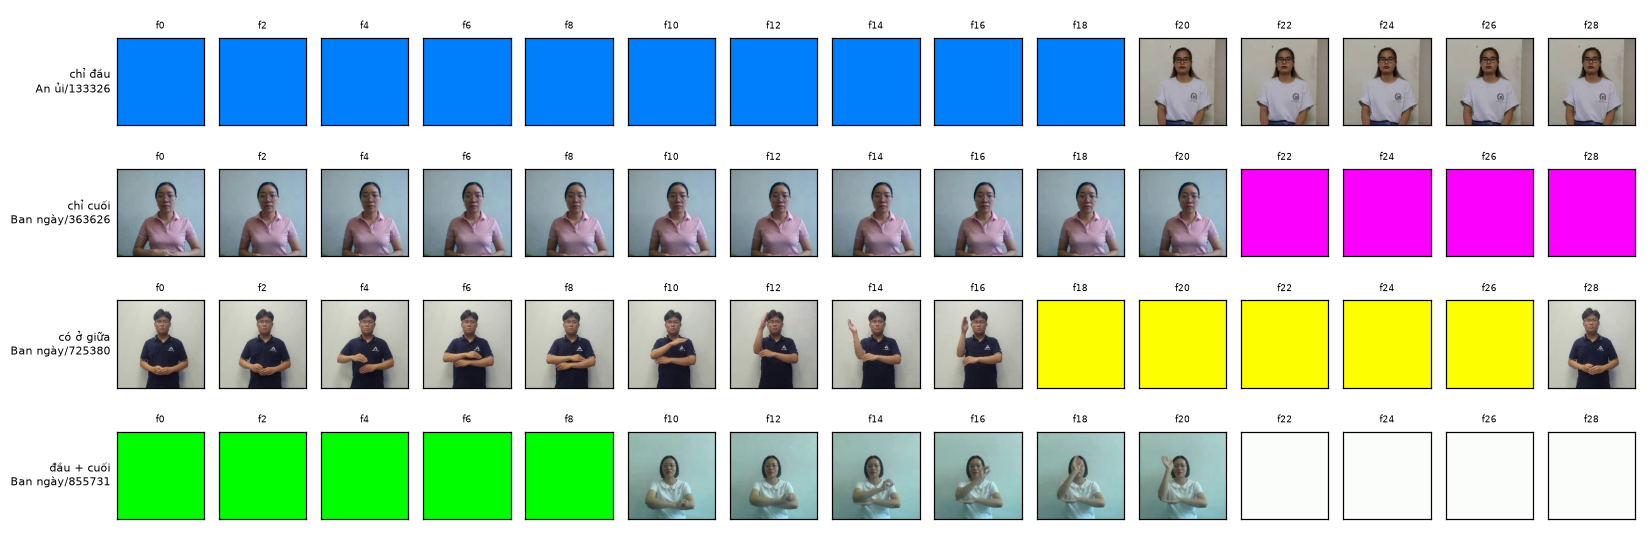
\includegraphics[width=\textwidth]{solid_frame_patterns.png}
  \caption{Bốn dạng khung đơn sắc trong tập train (khung chẵn $f_0$--$f_{28}$), mỗi dạng một video được chọn tự động: chỉ ở đầu (\textit{An ủi}/133326), chỉ ở cuối (\textit{Ban ngày}/363626), xen ở giữa (\textit{Ban ngày}/725380), cả đầu và cuối (\textit{Ban ngày}/855731).}
  \label{fig:eda_solid_examples}
\end{figure}

Hiện tượng này ảnh hưởng trực tiếp đến cách lấy mẫu: khi lấy $T=16$ khung đều nhau bằng \texttt{linspace} trên 565 video nói trên, trung bình có 6,4/16 khung được chọn là khung đơn sắc, và ở 224 video có từ 8/16 khung trở lên (ít nhất một nửa chuỗi đầu vào) là khung đơn sắc. Ngược lại, mỗi tập test chỉ có 1 video chứa đúng 1 khung đơn sắc. Như vậy khung đơn sắc là đặc điểm \emph{riêng của tập train}: nếu không xử lý, mô hình vừa mất thông tin ký hiệu, vừa có thể học các tín hiệu giả không tồn tại ở dữ liệu kiểm tra.

Sáu hàng đầu của Hình~\ref{fig:eda_suspicious} là các video có tỷ lệ khung đơn sắc cao nhất. Hai video được xác nhận bằng mắt là \textbf{rỗng hoàn toàn}: \texttt{Biết/214576.mp4} (2,5~KB, 16 khung, toàn màu xanh lục) và \texttt{Khai báo/885339.mp4} (2,7~KB, 23 khung, toàn màu xanh lam, kèm 2 bản sao \texttt{\_1}, \texttt{\_2}); cả hai không có người ký. Bốn video tiếp theo có 20--21/30 khung đơn sắc: \texttt{Nôn ói/915809}, \texttt{Thất lạc/708519}, \texttt{Chân/984642} và \texttt{Khai báo/362529}. Người ký chỉ xuất hiện trong khoảng 10 khung, ví dụ \texttt{Khai báo/362529} có 20 khung đỏ đầu tiên ($f_0$--$f_{19}$).

\paragraph{Giá trị ngoại lai} Nhóm dùng quy tắc Tukey (ngoài khoảng $[Q_1-1{,}5\,\mathrm{IQR},\,Q_3+1{,}5\,\mathrm{IQR}]$ tính trên tập train) cho thời lượng, dung lượng và FPS. Số lượng ngoại lai khá nhiều nhưng phần lớn chỉ lệch nhẹ (Mục~\ref{subsec:eda_uni}). Đáng chú ý là các ngoại lai cực đoan: thời lượng trên 5~s có 10 video train, 1 video public test và 3 video private test (lớn nhất 35,3~s ở train, 28,1~s ở private test); FPS dưới 5 có 9 video train và 2 video private test; dung lượng dưới 10~KB có 4 tệp train, đều là các video rỗng nói trên. Các ngoại lai này không nhất thiết là lỗi mà phản ánh việc video được lấy mẫu lại về $\approx$30 khung từ các clip gốc có độ dài rất khác nhau.

\paragraph{Nhiễu nhãn} Khi gom nhóm theo MD5, có hai nhóm nội dung giống hệt nhau nhưng nằm ở \emph{hai lớp khác nhau}: \texttt{Chậm lại/284430.mp4} trùng với \texttt{Chào/392683.mp4} và \texttt{Chào/468203.mp4}; \texttt{Chậm lại/254739.mp4} trùng với \texttt{Chào/792094.mp4}. Nhóm đã xem trực tiếp (Hình~\ref{fig:eda_suspicious}, năm hàng cuối) và xác nhận chúng có cùng người ký, cùng chuỗi động tác. Một video không thể đồng thời mang hai nghĩa nên ít nhất một trong hai nhãn là sai; tuy nhiên việc xác định nhãn đúng cần người am hiểu ngôn ngữ ký hiệu Việt Nam, nên báo cáo chỉ ghi nhận đây là \emph{xung đột nhãn}.

\begin{figure}[H]
  \centering
  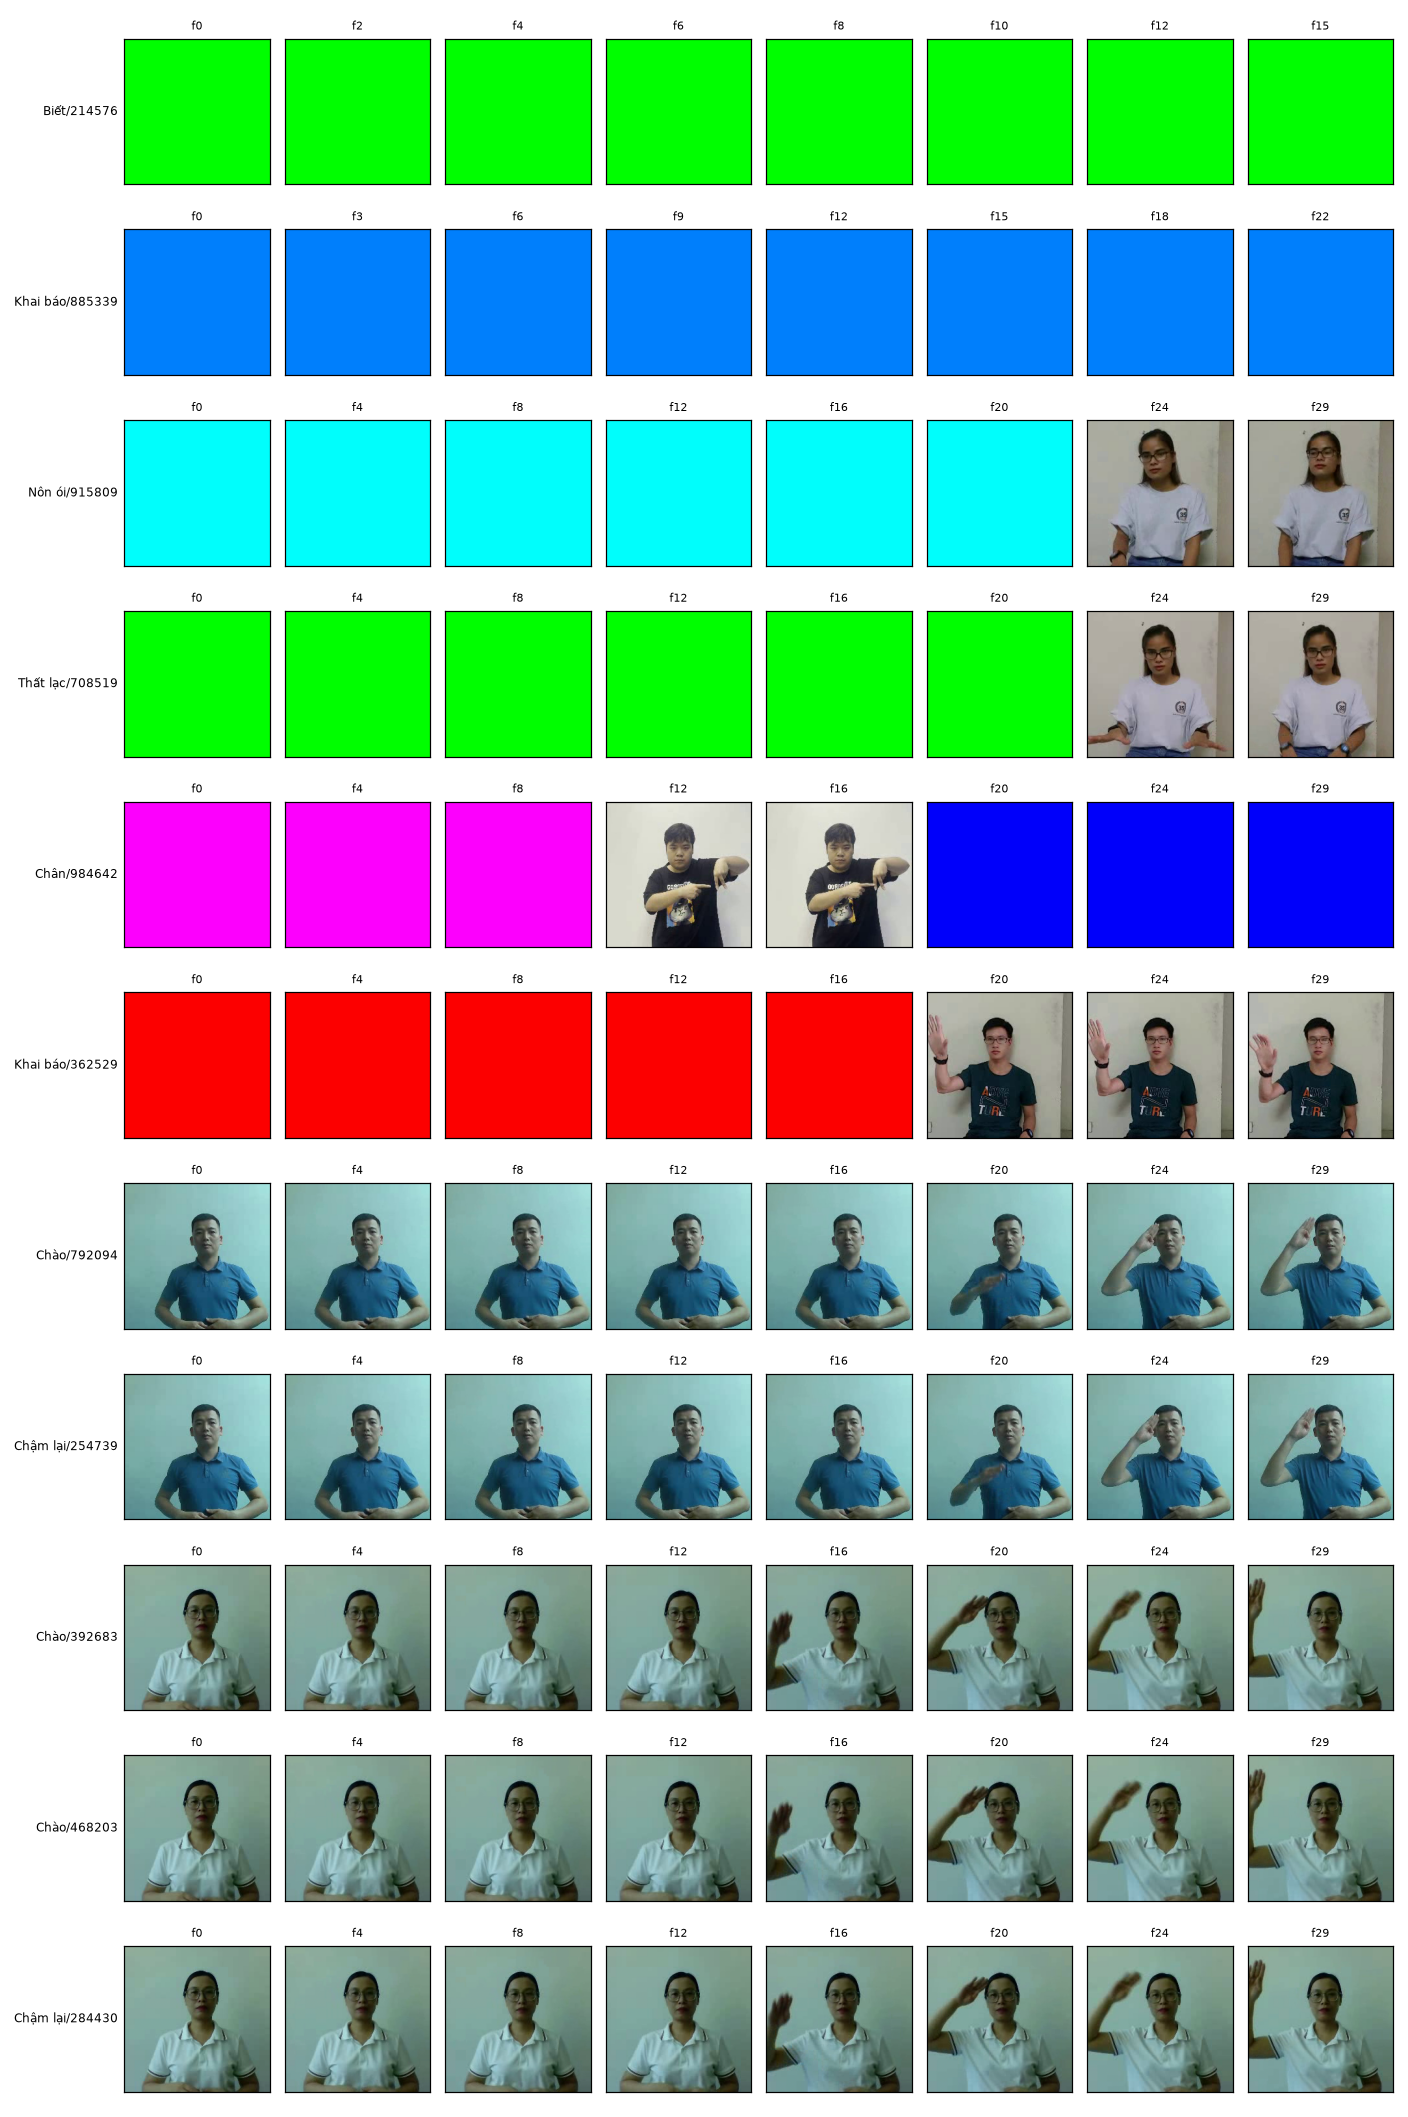
\includegraphics[width=0.9\textwidth,height=0.72\textheight,keepaspectratio]{flagged_videos_check.png}
  \caption{Kiểm tra bằng mắt các video do bước kiểm tra chất lượng tự đánh dấu. Sáu hàng đầu là các video có tỷ lệ khung đơn sắc cao nhất, gồm hai video rỗng hoàn toàn (\textit{Biết}/214576, \textit{Khai báo}/885339). Năm hàng cuối là hai nhóm video trùng nội dung nhưng khác nhãn (\textit{Chậm lại} $\leftrightarrow$ \textit{Chào}).}
  \label{fig:eda_suspicious}
\end{figure}

\paragraph{Trùng lặp giữa các tập} Public test có 8 bản trùng nội bộ (1.622 video duy nhất) và \textbf{157 video giống hệt video trong train}; private test có 2.782 video duy nhất, không trùng với train, nhưng có 896 video trùng với public test. Ngoài ra, 2.806 tên tệp trong private test trùng với tên tệp trong train nhưng nội dung hoàn toàn khác (MD5 khác, chênh lệch điểm ảnh lớn), nên đây chỉ là trùng cách đặt mã số; nguyên nhân chưa rõ và tên tệp \emph{không} được dùng để suy luận nhãn.

\noindent\textit{Hệ quả:} dữ liệu train chưa sạch; trước khi huấn luyện cần khử trùng lặp, loại video rỗng, xử lý khung đơn sắc và rà soát các nhãn xung đột. Điểm trên public test có thể bị ảnh hưởng một phần bởi 157 video đã có trong train.

% =====================================================================
\subsubsection{Phân tích đơn biến}
\label{subsec:eda_uni}

\paragraph{Script và cách thực hiện}
\begin{itemize}
  \item \textbf{Script:} \edafile{03\_univariate}{01\_numeric\_attributes.py}.
  \item \textbf{Cách khai thác dữ liệu:} với mỗi thuộc tính số (\texttt{frames}, \texttt{fps}, \texttt{dur}, \texttt{size\_kb}), script tính \texttt{groupby(\textquotesingle split\textquotesingle).describe()} (trung bình, độ lệch chuẩn, min, các tứ phân vị, max), hệ số lệch (\textit{skewness}) và các giá trị phổ biến nhất. Ngoại lai được xác định theo quy tắc Tukey với ngưỡng tính trên train rồi áp lên cả ba tập. Script vẽ histogram của từng thuộc tính cho ba tập trên cùng trục; histogram FPS và dung lượng dùng mật độ (\texttt{density=True}) để so sánh được các tập có kích thước khác nhau.
  \item \textbf{Đầu ra:} \texttt{desc\_by\_split.csv} (Bảng~\ref{tab:eda_desc}), \texttt{univariate\_summary.txt}, \texttt{frames\_hist\_by\_split.png}, \texttt{fps\_hist\_by\_split.png}, \texttt{filesize\_hist\_by\_split.png}.
\end{itemize}

Mục này khảo sát phân phối của từng thuộc tính số: số khung hình, FPS, thời lượng và dung lượng, tính trên từng tập (Bảng~\ref{tab:eda_desc}). Độ phân giải đã được trình bày ở Bảng~\ref{tab:eda_res}.

\begin{table}[H]
  \centering
  \caption{Thống kê mô tả các thuộc tính số theo từng tập.}
  \label{tab:eda_desc}
  \small
  \begin{tabular}{@{}llrrrrrrr@{}}
    \toprule
    \textbf{Thuộc tính} & \textbf{Tập} & \textbf{Mean} & \textbf{Std} & \textbf{Min} & \textbf{Q1} & \textbf{Median} & \textbf{Q3} & \textbf{Max} \\
    \midrule
    \multirow{3}{*}{Số khung}
      & train   & 29,88 & 1,26 & 16 & 30 & 30 & 30 & 30 \\
      & public  & 29,96 & 0,66 & 16 & 30 & 30 & 30 & 30 \\
      & private & 29,98 & 0,44 & 21 & 30 & 30 & 30 & 30 \\
    \midrule
    \multirow{3}{*}{FPS}
      & train   & 12,94 & 3,11 & 0,85 & 10,98 & 12,34 & 14,06 & 30,02 \\
      & public  & 12,97 & 3,00 & 5,93 & 10,98 & 12,50 & 13,85 & 30,00 \\
      & private & 13,32 & 3,69 & 1,07 & 10,84 & 12,50 & 14,06 & 30,02 \\
    \midrule
    \multirow{3}{*}{Thời lượng (s)}
      & train   & 2,48 & 1,36 & 0,70 & 2,13 & 2,43 & 2,73 & 35,29 \\
      & public  & 2,42 & 0,51 & 0,70 & 2,17 & 2,40 & 2,73 & 5,06 \\
      & private & 2,42 & 0,82 & 0,70 & 2,13 & 2,40 & 2,77 & 28,14 \\
    \midrule
    \multirow{3}{*}{Dung lượng (KB)}
      & train   & 85,5  & 38,5 & 2,5  & 60,2 & 80,6 & 103,0 & 263,8 \\
      & public  & 113,6 & 77,5 & 26,2 & 76,1 & 91,0 & 125,8 & 483,2 \\
      & private & 116,3 & 77,7 & 42,2 & 77,7 & 94,6 & 126,0 & 488,0 \\
    \bottomrule
  \end{tabular}
\end{table}

\paragraph{Số khung hình} Hầu hết video có đúng 30 khung: 3.832/3.875 video train (98,9\%), 1.623/1.630 public test và 2.850/2.859 private test; ở train có 26 video chỉ có 16 khung. Không video nào ngắn hơn 16 khung (Hình~\ref{fig:eda_frames_hist}), nên không cần đệm khung thực sự khi lấy $T=16$.

\begin{figure}[H]
  \centering
  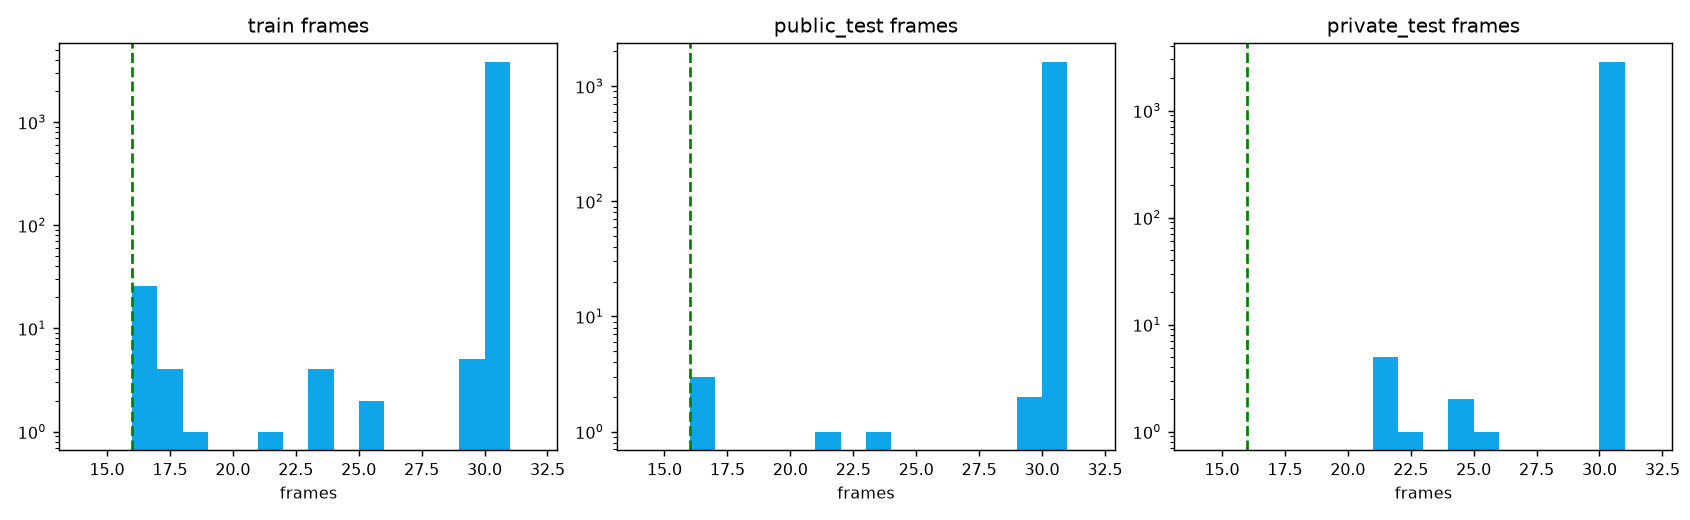
\includegraphics[width=\textwidth]{frames_hist_by_split.png}
  \caption{Histogram số khung hình mỗi video theo tập (trục tung thang log). Đường đứt nét đánh dấu $T=16$.}
  \label{fig:eda_frames_hist}
\end{figure}

\paragraph{FPS và thời lượng} Dù số khung gần như cố định, FPS biến thiên mạnh: train có 961 giá trị FPS khác nhau, từ 0,85 đến 30,02 (trung vị 12,3), phân phối lệch phải với đuôi dài (hệ số lệch 1,01 ở train; Hình~\ref{fig:eda_fps_hist}). Vì thời lượng $=\texttt{frames}/\texttt{fps}$ nên thời lượng thực của cùng 30 khung dao động lớn: trung vị khoảng 2,4~s nhưng có video tới 35,3~s ở train và 28,1~s ở private test, trong khi 99\% video đều ngắn hơn khoảng 4~s. Điều này cho thấy video đã được lấy mẫu lại về khoảng 30 khung bất kể độ dài clip gốc.

\begin{figure}[H]
  \centering
  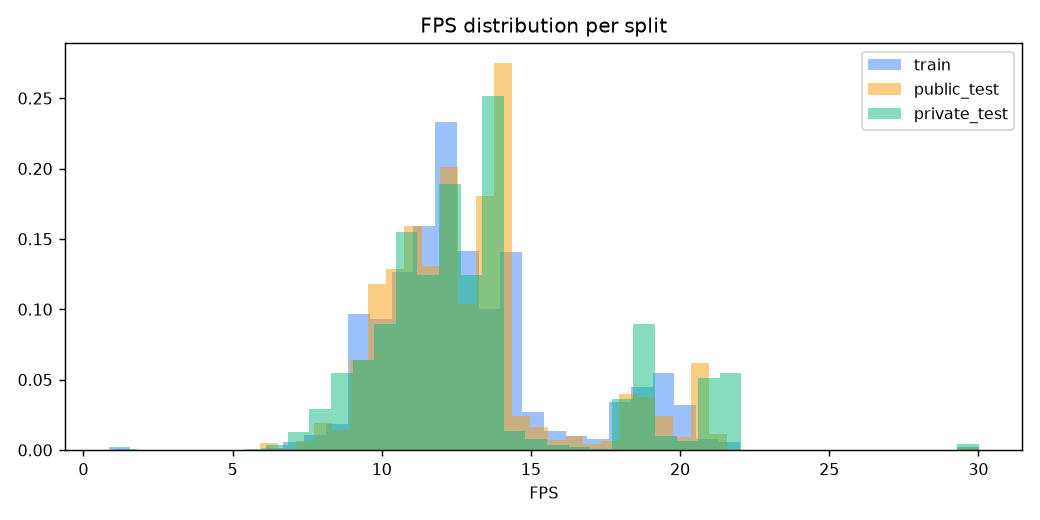
\includegraphics[width=0.85\textwidth]{fps_hist_by_split.png}
  \caption{Phân phối FPS theo từng tập.}
  \label{fig:eda_fps_hist}
\end{figure}

\paragraph{Dung lượng tệp} Dung lượng train có trung vị 80,6~KB (trung bình 85,5; từ 2,5 đến 263,8~KB). Hai tập test có phân phối lệch phải hơn hẳn: trung bình 113,6--116,3~KB, lớn nhất tới 483--488~KB (Hình~\ref{fig:eda_size_hist}); khác biệt này được phân tích ở Mục~\ref{subsec:eda_shift}.

\begin{figure}[H]
  \centering
  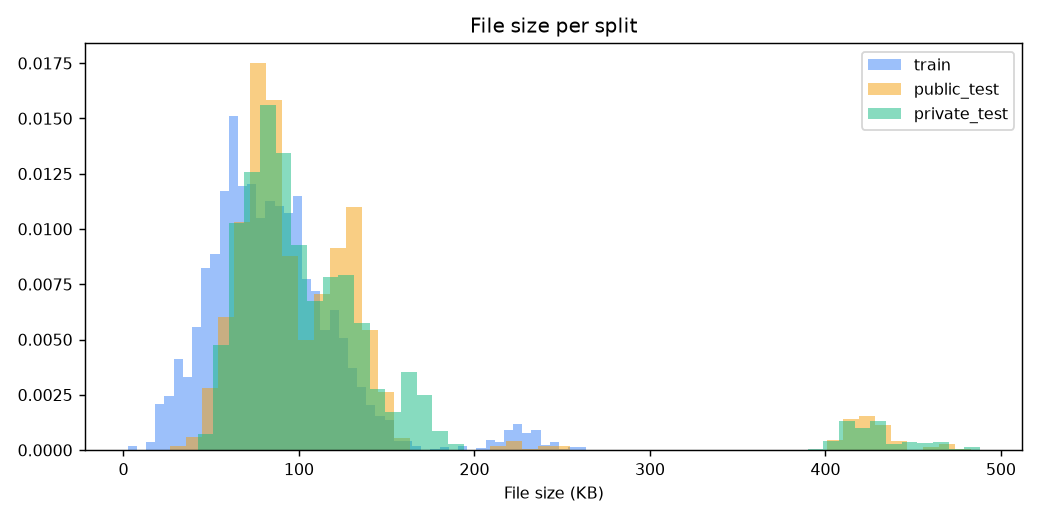
\includegraphics[width=0.85\textwidth]{filesize_hist_by_split.png}
  \caption{Phân phối dung lượng tệp (KB) theo từng tập.}
  \label{fig:eda_size_hist}
\end{figure}

\noindent\textit{Hệ quả:} (i) không cần đổi kích thước khung hình, tuy kiến trúc CRNN với \texttt{Adaptive\allowbreak AvgPool2d} vẫn đảm bảo tính tổng quát nếu gặp video khác độ phân giải; (ii) vì mọi video có ít nhất 16 khung, lấy mẫu $T=16$ khung đều nhau bằng \texttt{linspace} (\textit{Frame Downsampling}) là đủ, lặp khung (\textit{repeat padding}) chỉ giữ làm phương án dự phòng; (iii) phân phối FPS và dung lượng lệch phải với nhiều ngoại lai nên nên dùng trung vị thay vì trung bình khi mô tả.

% =====================================================================
\subsubsection{Phân tích biến mục tiêu}
\label{subsec:eda_class}

\paragraph{Script và cách thực hiện}
\begin{itemize}
  \item \textbf{Script:} \edafile{04\_target\_analysis}{01\_class\_distribution.py}.
  \item \textbf{Cách khai thác dữ liệu:} lọc các dòng của tập train trong \texttt{video\_metadata.csv}, đếm số video mỗi nhãn bằng \texttt{value\_counts()}, sau đó tính trung bình, trung vị, độ lệch chuẩn, tỷ lệ lớp lớn nhất/nhỏ nhất và số lớp có không quá 25 hoặc từ 50 video trở lên. Số video mỗi lớp sau khử trùng lặp lấy từ \texttt{class\_counts\_train\_unique\_vs\_all.csv} của bước \texttt{02\_data\_quality}.
  \item \textbf{Đầu ra:} \texttt{class\_summary.txt}, \texttt{class\_counts\_train.csv}, \texttt{class\_distribution\_all.png}, \texttt{class\_top\_bottom10.png}, \texttt{samples\_per\_class\_hist.png}.
\end{itemize}

Nhóm dùng \texttt{value\_counts()} trên cột nhãn của tập \texttt{train} để đếm số video mỗi lớp, rồi vẽ biểu đồ cho cả 100 lớp (Hình~\ref{fig:eda_class_dist}), 10 lớp nhiều nhất/ít nhất (Hình~\ref{fig:eda_top_bottom}) và histogram số video mỗi lớp (Hình~\ref{fig:eda_spc_hist}).

\begin{figure}[H]
  \centering
  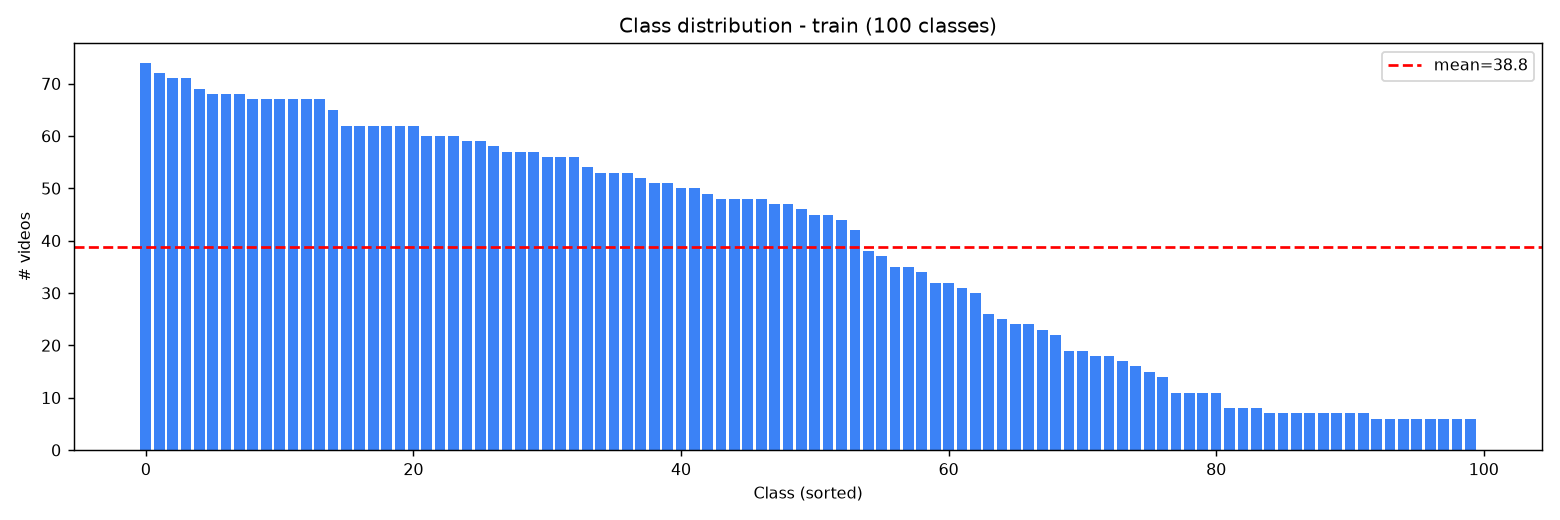
\includegraphics[width=\textwidth]{class_distribution_all.png}
  \caption{Phân phối số video theo lớp trong tập huấn luyện (100 lớp, sắp xếp giảm dần).}
  \label{fig:eda_class_dist}
\end{figure}

Tập huấn luyện gồm 3.875 video nhưng phân bố không đồng đều: trung bình 38,75 video/lớp, trung vị 45,5, độ lệch chuẩn 22,78. Lớp nhiều nhất (\textit{Trường học}) có 74 video, trong khi mười lớp chỉ có 6--7 video; tỷ lệ chênh giữa lớp lớn nhất và nhỏ nhất xấp xỉ $12{,}3$ lần (Bảng~\ref{tab:eda_top_bottom}). Có 36/100 lớp có không quá 25 video và 42/100 lớp có từ 50 video trở lên, tức phân phối có dạng hai đỉnh: nhóm lớp ``giàu'' (khoảng 45--74 video) và nhóm lớp ``nghèo'' (khoảng 6--11 video). Nhiều lớp ít mẫu thuộc nhóm từ vựng y tế -- dịch bệnh.

\begin{table}[H]
  \centering
  \caption{Mười lớp nhiều mẫu nhất và mười lớp ít mẫu nhất trong tập huấn luyện.}
  \label{tab:eda_top_bottom}
  \begin{tabular}{@{}lr@{\hspace{2.5em}}lr@{}}
    \toprule
    \multicolumn{2}{c}{\textbf{Nhiều nhất}} & \multicolumn{2}{c}{\textbf{Ít nhất}} \\
    \cmidrule(r){1-2}\cmidrule(l){3-4}
    \textbf{Lớp} & \textbf{Số video} & \textbf{Lớp} & \textbf{Số video} \\
    \midrule
    Trường học & 74 & Nhầm      & 7 \\
    Rau        & 72 & Virus     & 7 \\
    Nhà        & 71 & Bệnh nhân & 6 \\
    Áp dụng    & 71 & Cách ly   & 6 \\
    Chậm lại   & 69 & Cơ thể    & 6 \\
    Cám dỗ     & 68 & Ho        & 6 \\
    Nghe       & 68 & Phục hồi  & 6 \\
    Nói xấu    & 68 & Sốt       & 6 \\
    Biết       & 67 & Xe máy    & 6 \\
    Chạy       & 67 & Ủng hộ    & 6 \\
    \bottomrule
  \end{tabular}
\end{table}

\begin{figure}[H]
  \centering
  \begin{minipage}{0.56\textwidth}
    \centering
    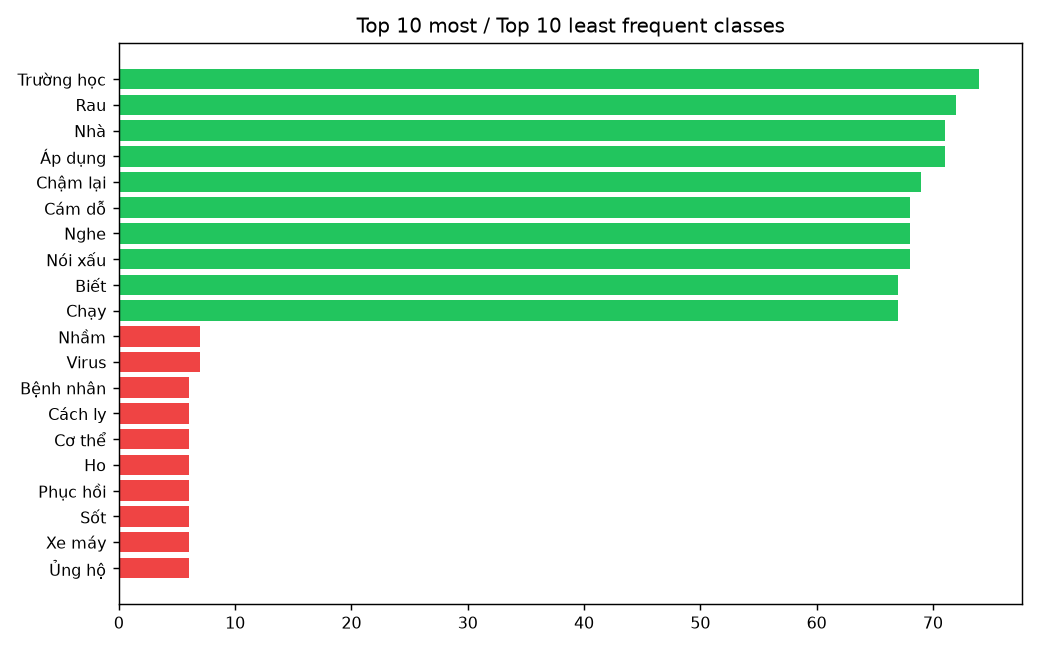
\includegraphics[width=\textwidth]{class_top_bottom10.png}
    \caption{Mười lớp nhiều nhất (xanh) và ít nhất (đỏ).}
    \label{fig:eda_top_bottom}
  \end{minipage}\hfill
  \begin{minipage}{0.42\textwidth}
    \centering
    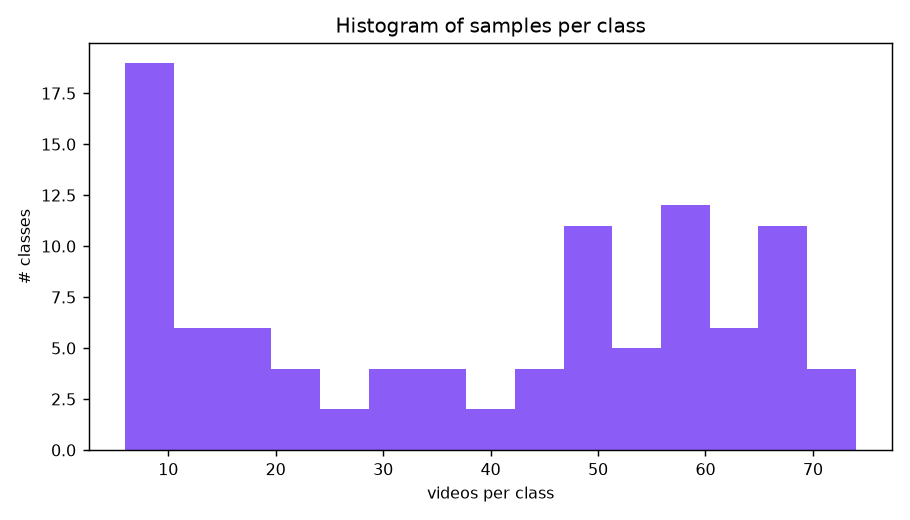
\includegraphics[width=\textwidth]{samples_per_class_hist.png}
    \caption{Histogram số video mỗi lớp.}
    \label{fig:eda_spc_hist}
  \end{minipage}
\end{figure}

Các con số trên tính trên tệp gốc, \emph{chưa} khử trùng lặp.

\noindent\textit{Hệ quả:} dữ liệu bị mất cân bằng lớp (\textit{Class Imbalance}) rõ rệt. Nếu đánh giá bằng Accuracy, mô hình có thể thiên về lớp phổ biến mà vẫn đạt điểm cao; vì vậy dùng Macro F1 (cũng là thước đo chính thức) và cần biện pháp xử lý mất cân bằng ở bước tiền xử lý/huấn luyện.

% =====================================================================
\subsubsection{Phân tích hai biến và đa biến}
\label{subsec:eda_multi}

\paragraph{Script và cách thực hiện}
\begin{itemize}
  \item \textbf{Script:} \edafile{05\_bivariate\_multivariate}{01\_correlation\_and\_label\_association.py}.
  \item \textbf{Cách khai thác dữ liệu:} ghép \texttt{video\_metadata.csv} với \texttt{video\_quality\_flags.csv} theo khoá (tập, lớp, tên tệp); bỏ các bản sao \texttt{\_N} để chỉ giữ 2.776 video duy nhất của train. Tính ma trận tương quan Pearson và Spearman (tương quan hạng, ít nhạy với ngoại lai) giữa các thuộc tính số; với từng thuộc tính, chia giá trị theo 100 lớp rồi chạy kiểm định Kruskal--Wallis (\texttt{scipy.stats.kruskal}) và tính $\eta^2 = SS_{\text{giữa lớp}}/SS_{\text{tổng}}$. Trung vị và tứ phân vị FPS của từng lớp được sắp xếp tăng dần để vẽ.
  \item \textbf{Đầu ra:} \texttt{multivariate\_summary.txt}, \texttt{corr\_heatmap.png}, \texttt{fps\_by\_class.png}, \texttt{size\_vs\_solid.png}.
\end{itemize}

Vì dữ liệu video không có đặc trưng dạng bảng, phân tích hai biến và đa biến tập trung vào mối quan hệ giữa các thuộc tính metadata với nhau và với nhãn lớp. Để tránh bản sao làm lệch kết quả, các phép tính dưới đây dùng 2.776 video duy nhất của tập train.

\paragraph{Tương quan giữa các thuộc tính} Hình~\ref{fig:eda_corr} cho thấy hệ số tương quan Pearson giữa số khung, FPS, dung lượng, tỷ lệ khung đơn sắc và độ chuyển động. (Thời lượng không đưa vào vì $\texttt{dur}=\texttt{frames}/\texttt{fps}$ nên phụ thuộc hoàn toàn vào hai biến còn lại.) Hầu hết các cặp có tương quan yếu ($|r|<0{,}35$); hai quan hệ rõ nhất là dung lượng -- tỷ lệ khung đơn sắc ($r\approx-0{,}45$; Spearman $\rho\approx-0{,}51$) và FPS -- chuyển động ($r\approx-0{,}34$; $\rho\approx-0{,}30$). Tương quan Spearman cho cùng chiều và độ lớn tương tự, nên các quan hệ này không phải do ngoại lai tạo ra. Quan hệ đầu là hợp lý: khung đơn sắc nén rất nhỏ nên video chứa nhiều khung đơn sắc có dung lượng thấp (Hình~\ref{fig:eda_size_solid}). Quan hệ sau cho thấy video có FPS thấp (clip gốc dài hơn) có độ chuyển động giữa các khung liên tiếp lớn hơn. Số khung gần như không liên quan tới các biến khác vì hầu như không đổi.

\begin{figure}[H]
  \centering
  \begin{minipage}{0.48\textwidth}
    \centering
    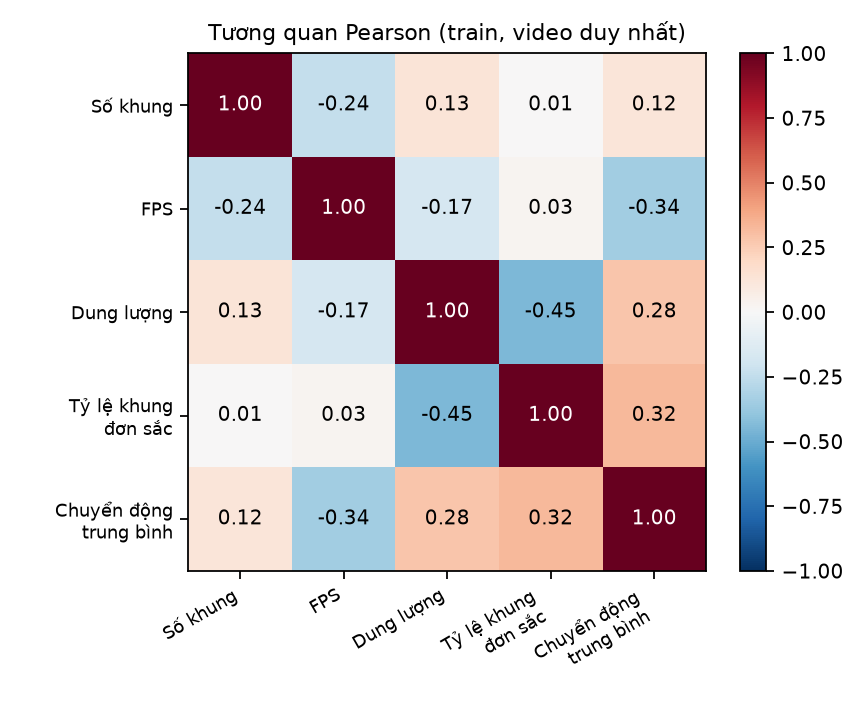
\includegraphics[width=\textwidth]{corr_heatmap.png}
    \caption{Ma trận tương quan Pearson giữa các thuộc tính (train, video duy nhất).}
    \label{fig:eda_corr}
  \end{minipage}\hfill
  \begin{minipage}{0.48\textwidth}
    \centering
    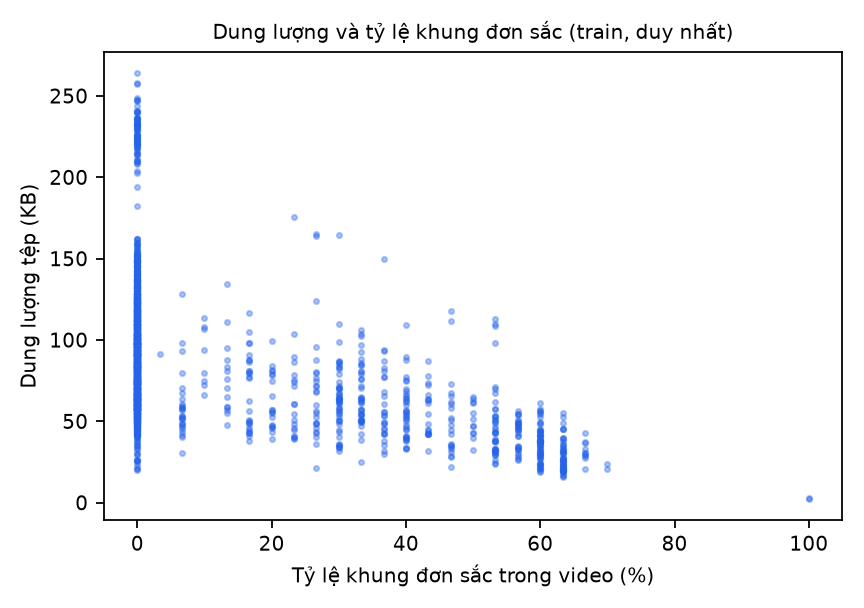
\includegraphics[width=\textwidth]{size_vs_solid.png}
    \caption{Dung lượng tệp theo tỷ lệ khung đơn sắc.}
    \label{fig:eda_size_solid}
  \end{minipage}
\end{figure}

\paragraph{Quan hệ giữa thuộc tính và nhãn lớp} Nhóm so sánh phân phối của từng thuộc tính giữa 100 lớp bằng kiểm định Kruskal--Wallis và hệ số $\eta^2$ (tỷ lệ phương sai giải thích bởi nhãn). Kết quả: FPS có $\eta^2\approx0{,}28$, dung lượng $\eta^2\approx0{,}15$, số khung $\eta^2\approx0{,}08$; cả ba đều có $p<10^{-10}$. Nói cách khác, FPS của video khác nhau rõ rệt giữa các lớp: trung vị FPS của lớp dao động từ khoảng 9,4 (\textit{Ngón tay}) đến khoảng 19,2 (\textit{Ho}), trong khi trung vị toàn tập là 12,4 (Hình~\ref{fig:eda_fps_class}). Điều này gợi ý rằng thời lượng clip gốc (và do đó FPS sau khi lấy mẫu lại) có liên hệ với từ được ký -- có thể vì các từ khác nhau có độ dài tự nhiên khác nhau -- hoặc vì cách thu thập dữ liệu theo từng lớp. Nhóm chưa xác định được nguyên nhân.

\begin{figure}[H]
  \centering
  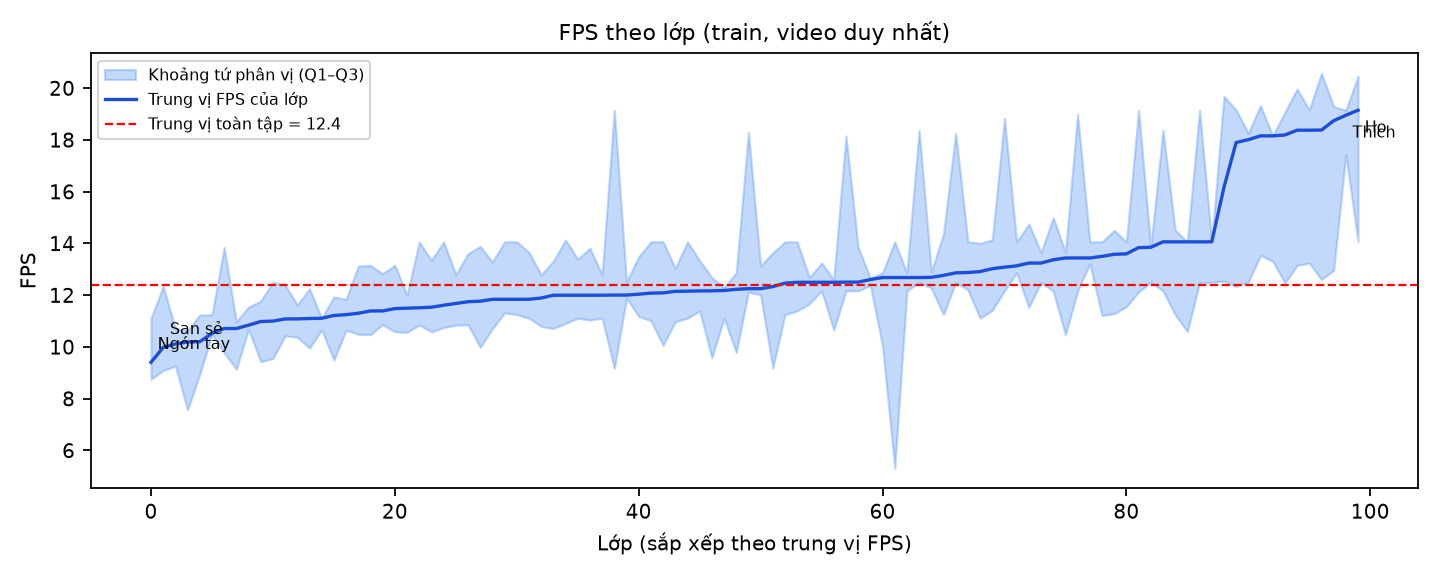
\includegraphics[width=0.95\textwidth]{fps_by_class.png}
  \caption{Trung vị và khoảng tứ phân vị của FPS theo lớp (train, video duy nhất), các lớp sắp xếp theo trung vị.}
  \label{fig:eda_fps_class}
\end{figure}

\paragraph{Khung đơn sắc theo lớp} Khung đơn sắc không phân bố đều: 78/100 lớp có ít nhất một video bị ảnh hưởng, và có lớp có tới 30--40\% video duy nhất chứa khung đơn sắc (\textit{Có thể}, \textit{Xin lỗi}, \textit{Thất lạc}, \textit{Mua}). Do đó việc loại bỏ khung đơn sắc sẽ tác động không đồng đều lên các lớp.

\noindent\textit{Hệ quả:} (i) các thuộc tính metadata phần lớn độc lập nhau nên không có cặp đặc trưng dư thừa cần loại bỏ; (ii) vì FPS và dung lượng có quan hệ thống kê với nhãn, chúng có thể trở thành ``đường tắt'' (\textit{shortcut}) mà mô hình học được thay vì học ký hiệu, nên không nên đưa FPS hoặc dung lượng làm đặc trưng đầu vào và cần theo dõi nguy cơ này khi đánh giá; (iii) cần kiểm tra lại phân phối nhãn sau khi loại khung đơn sắc.

% =====================================================================
\subsubsection{So sánh phân phối giữa các tập}
\label{subsec:eda_shift}

\paragraph{Script và cách thực hiện}
\begin{itemize}
  \item \textbf{Script:} \edafile{06\_split\_comparison}{01\_split\_shift.py}.
  \item \textbf{Cách khai thác dữ liệu:} với train chỉ giữ video duy nhất, để các bản sao không làm lệch phân phối. Với mỗi thuộc tính (\texttt{frames}, \texttt{fps}, \texttt{dur}, \texttt{size\_kb}, \texttt{motion}), script tính trung vị từng tập và chạy kiểm định Kolmogorov--Smirnov hai mẫu (\texttt{scipy.stats.ks\_2samp}) cho từng cặp tập. Thống kê $D$ là khoảng cách lớn nhất giữa hai hàm phân phối tích luỹ thực nghiệm (ECDF); $D$ càng lớn thì hai phân phối càng khác nhau. Script cũng tính tỷ lệ video có khung đơn sắc ở từng tập và số video trùng nội dung giữa các tập (theo \texttt{file\_hashes.csv}). Ngưỡng ngoại lai trên của dung lượng (167~KB, tính từ train) lấy từ bước đơn biến.
  \item \textbf{Đầu ra:} \texttt{split\_shift\_summary.txt}, \texttt{ecdf\_by\_split.png}.
\end{itemize}

Nhóm so sánh phân phối các thuộc tính giữa ba tập trên cùng trục (Bảng~\ref{tab:eda_desc}, Bảng~\ref{tab:eda_ks}, Hình~\ref{fig:eda_ecdf}) để tìm dấu hiệu khác biệt miền (\textit{Domain Shift}).

\begin{table}[H]
  \centering
  \caption{Kiểm định Kolmogorov--Smirnov hai mẫu giữa các tập (train: video duy nhất). Giá trị là thống kê $D$, trong ngoặc là $p$-value.}
  \label{tab:eda_ks}
  \small
  \begin{tabular}{@{}lccc@{}}
    \toprule
    \textbf{Thuộc tính} & \textbf{train -- public} & \textbf{train -- private} & \textbf{public -- private} \\
    \midrule
    Số khung        & 0,005 (1)                 & 0,007 (1)                 & 0,002 (1) \\
    FPS             & 0,075 ($1{,}7\cdot10^{-5}$) & 0,069 ($2{,}9\cdot10^{-6}$) & 0,094 ($1{,}7\cdot10^{-8}$) \\
    Thời lượng      & 0,075 ($1{,}7\cdot10^{-5}$) & 0,068 ($4{,}5\cdot10^{-6}$) & 0,094 ($1{,}7\cdot10^{-8}$) \\
    Dung lượng      & \textbf{0,230} ($2\cdot10^{-48}$) & \textbf{0,237} ($4\cdot10^{-70}$) & 0,059 (0,0013) \\
    Chuyển động     & 0,059 (0,0015)            & 0,079 ($4{,}8\cdot10^{-8}$) & 0,035 (0,15) \\
    \bottomrule
  \end{tabular}
\end{table}

\begin{figure}[H]
  \centering
  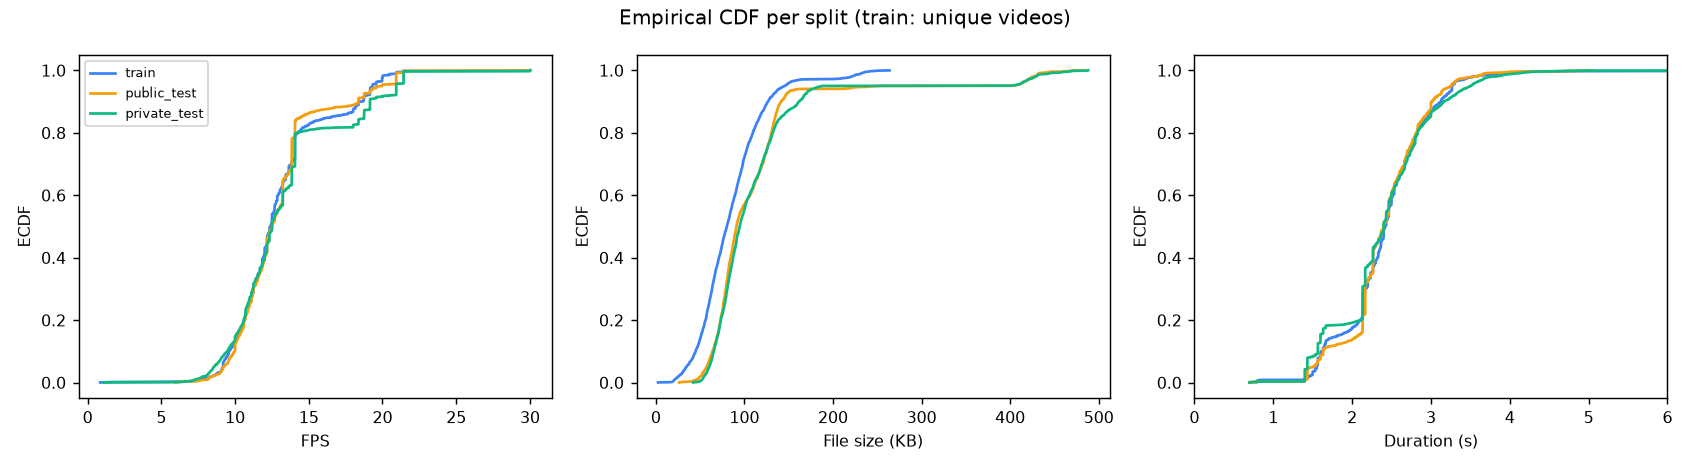
\includegraphics[width=\textwidth]{ecdf_by_split.png}
  \caption{Hàm phân phối tích luỹ thực nghiệm của FPS, dung lượng và thời lượng theo tập (train: video duy nhất). Đường dung lượng của train tách hẳn khỏi hai tập test.}
  \label{fig:eda_ecdf}
\end{figure}

Vì cỡ mẫu lớn nên mọi khác biệt dù nhỏ đều có $p$ rất bé; nhóm đánh giá chủ yếu theo độ lớn của $D$. Số khung hình giống nhau ở cả ba tập ($D<0{,}01$), độ phân giải cũng vậy. FPS, thời lượng và độ chuyển động khác biệt nhỏ ($D<0{,}1$). Riêng dung lượng khác biệt rõ giữa train và hai tập test ($D\approx0{,}23$--$0{,}24$), trong khi hai tập test gần nhau ($D\approx0{,}06$). Cụ thể:

\begin{itemize}
  \item \textbf{Dung lượng:} video test nặng hơn đáng kể (trung bình 113,6--116,3~KB so với 85,5~KB; trung vị 91,0--94,6~KB so với 80,6~KB). Tỷ lệ video vượt 167~KB (ngưỡng ngoại lai của train) là 3,1\% ở train nhưng 6,0\% ở public và 8,2\% ở private. Một phần chênh lệch có thể giải thích bởi khung đơn sắc (nén rất nhỏ) chỉ có ở train: trung vị dung lượng của video train có khung đơn sắc là 49,0~KB, còn của video train không có khung đơn sắc là 87,6~KB, gần mức của test. Tuy nhiên đuôi dài tới 488~KB ở test không xuất hiện ở train (lớn nhất 263,8~KB), cho thấy test có thể chứa các video chi tiết hoặc nhiễu hơn.
  \item \textbf{FPS:} trung vị gần như nhau (12,4 ở train, 12,5 ở hai tập test), nhưng private test có độ lệch chuẩn lớn hơn (3,69 so với 3,11 ở train) và đuôi dài hơn.
  \item \textbf{Khung đơn sắc:} khoảng 20\% video train nhưng gần như không có ở test (Bảng~\ref{tab:eda_solid}).
  \item \textbf{Người ký, nền, ánh sáng:} có thể khác giữa train và test; nhóm chưa định lượng được yếu tố này.
\end{itemize}

\noindent\textit{Hệ quả:} cần các phép tăng cường giúp mô hình bền vững với thay đổi màu sắc, độ sáng và khung cắt (\textit{ColorJitter}, \textit{Random Resized Crop}); việc loại bỏ khung đơn sắc ở train đồng thời giúp thu hẹp khoảng cách giữa phân phối train và test.

% =====================================================================
\subsubsection{Kết luận EDA và khuyến nghị cho bước tiền xử lý}
\label{subsec:eda_conclusion}

Bảng~\ref{tab:eda_reco} tổng hợp các vấn đề phát hiện được, bằng chứng và khuyến nghị cho bước tiền xử lý (Mục~\ref{sec:preprocess}) cũng như huấn luyện.

\begin{table}[H]
  \centering
  \caption{Tổng hợp vấn đề, bằng chứng và khuyến nghị cho bước tiền xử lý.}
  \label{tab:eda_reco}
  \small
  \begin{tabular}{@{}p{0.2\textwidth}p{0.36\textwidth}p{0.38\textwidth}@{}}
    \toprule
    \textbf{Vấn đề} & \textbf{Bằng chứng} & \textbf{Khuyến nghị} \\
    \midrule
    Tên lớp khác dạng Unicode & Khoá trong \texttt{label\_mapping.pkl} ở dạng NFD, thư mục lớp ở dạng NFC; 91/100 lớp không khớp nếu so nguyên văn & Chuẩn hoá NFC cả hai phía trước khi tra nhãn \\
    \addlinespace
    Video trùng lặp (\texttt{\_N}) & 1.069 tệp \texttt{\_N} giống hệt bản gốc; chỉ còn 2.776 video duy nhất & Khử trùng lặp theo MD5; chia train/validation theo ID gốc (bỏ hậu tố \texttt{\_N}) bằng \texttt{StratifiedGroupKFold} để tránh rò rỉ \\
    \addlinespace
    Mất cân bằng lớp & 6--74 video/lớp (sau khử trùng lặp: 5--51), 36/100 lớp có $\leq$25 video & Dùng Macro F1; trọng số lớp hoặc \texttt{WeightedRandomSampler}; oversample kèm tăng cường cho lớp ít mẫu; có thể dùng label smoothing \\
    \addlinespace
    Khung đơn sắc & 565/2.776 video duy nhất (20,4\%) chứa trung bình 12,2 khung đơn sắc; test gần như không có & Loại bỏ khung đơn sắc (độ lệch chuẩn điểm ảnh $<3$) \emph{trước} khi lấy mẫu $T=16$; nếu còn ít hơn 16 khung hợp lệ thì lặp khung \\
    \addlinespace
    Video rỗng & \texttt{Biết/214576}, \texttt{Khai báo/885339} (cùng 2 bản sao) đơn sắc toàn bộ & Loại khỏi tập huấn luyện \\
    \addlinespace
    Xung đột nhãn & 2 nhóm nội dung giống hệt nhưng thuộc \textit{Chậm lại} và \textit{Chào} & Xác minh nhãn đúng; nếu không xác minh được thì loại bỏ \\
    \addlinespace
    Độ dài không đồng nhất & 98,9\% video có 30 khung, tối thiểu 16 khung; thời lượng tới 35,3~s & Lấy mẫu $T=16$ khung đều bằng \texttt{linspace} \\
    \addlinespace
    FPS/dung lượng liên hệ với nhãn & $\eta^2\approx0{,}28$ (FPS), $0{,}15$ (dung lượng) giữa các lớp & Không dùng FPS, dung lượng làm đặc trưng; theo dõi nguy cơ shortcut \\
    \addlinespace
    Khác biệt miền train--test & Test nặng hơn (trung bình 114--116~KB so với 85,5~KB; KS $D\approx0{,}23$); khung đơn sắc chỉ có ở train & ColorJitter, Random Resized Crop, chuẩn hoá ImageNet; \emph{không} lật ngang \\
    \addlinespace
    Trùng train--public test & 157 video public giống hệt video train & Lưu ý khi diễn giải điểm public test \\
    \bottomrule
  \end{tabular}
\end{table}

Tóm lại, bộ dữ liệu có định dạng rất đồng nhất (100\% video $224\times224$, gần như đều 30 khung), nên khâu đọc và lấy mẫu khung đơn giản. Tuy nhiên dữ liệu huấn luyện có ba vấn đề cần xử lý trước khi huấn luyện: mất cân bằng lớp, khoảng 28\% tệp là bản sao gây nguy cơ rò rỉ dữ liệu, và khoảng 20\% video chứa khung đơn sắc vốn không xuất hiện ở dữ liệu kiểm tra. Đây là những yếu tố có thể khiến điểm validation cao hơn đáng kể so với điểm thực tế trên tập kiểm tra nếu không được xử lý.

\paragraph{Hạn chế của phân tích} FPS và thời lượng đọc từ metadata của container nên có thể không phản ánh tốc độ quay thực. Ngưỡng độ lệch chuẩn $<3$ chỉ phát hiện khung đơn sắc hoàn toàn, chưa phát hiện khung mờ hoặc chỉ có nền. Nhóm chưa định lượng sự khác biệt về người ký và bối cảnh giữa train và test, chưa xác định được nguyên nhân FPS liên hệ với nhãn, và chưa xác định được nhãn đúng cho các video xung đột.
]
% Cấu trúc theo khung EDA chuẩn:
%   3.1.1 Mục tiêu và tổng quan dữ liệu
%   3.1.2 Cấu trúc dữ liệu
%   3.1.3 Chất lượng dữ liệu
%   3.1.4 Phân tích đơn biến
%   3.1.5 Phân tích biến mục tiêu
%   3.1.6 Phân tích hai biến và đa biến
%   3.1.7 So sánh phân phối giữa các tập
%   3.1.8 Kết luận và khuyến nghị
% Gói cần: graphicx, booktabs, float, caption, amsmath
% =====================================================================

\subsection{Phân tích dữ liệu (EDA)}
\label{sec:eda}

% \edafile{thư mục}{tệp}: in đường dẫn script, cho phép xuống dòng sau dấu /
\newcommand{\edafile}[2]{\texttt{#1/}\allowbreak\texttt{#2}}
% Cho phép xuống dòng sau dấu gạch dưới trong tên tệp dài (vd. class\_counts\_train\_unique\_vs\_all.csv)
\let\edaOrigUS\_
\renewcommand{\_}{\edaOrigUS\allowbreak}
\sloppy

Mục này trình bày kết quả phân tích khám phá dữ liệu (\textit{Exploratory Data Analysis -- EDA}) trên bộ dữ liệu video ngôn ngữ ký hiệu. EDA chỉ nhằm \emph{quan sát} xu hướng, phân phối và chất lượng dữ liệu. Nhóm sử dụng Python làm công cụ để thực hiện EDA (\texttt{os}, \texttt{pickle}, \texttt{pandas}, \texttt{OpenCV}, \texttt{numpy}, \texttt{hashlib}, \texttt{matplotlib}).

Phần phân tích được tổ chức theo trình tự quy trình EDA: tổng quan và cấu trúc dữ liệu (Mục~\ref{subsec:eda_overview}--\ref{subsec:eda_structure}), chất lượng dữ liệu (Mục~\ref{subsec:eda_quality}), phân tích đơn biến (Mục~\ref{subsec:eda_uni}), phân tích biến mục tiêu (Mục~\ref{subsec:eda_class}), phân tích hai biến và đa biến (Mục~\ref{subsec:eda_multi}), so sánh giữa các tập (Mục~\ref{subsec:eda_shift}) và cuối cùng là kết luận kèm khuyến nghị (Mục~\ref{subsec:eda_conclusion}).

\begin{table}[H]
  \centering
  \caption{Các script EDA, thứ tự chạy và mục sử dụng kết quả.}
  \label{tab:eda_scripts}
  \small
  \begin{tabular}{@{}p{0.17\textwidth}p{0.26\textwidth}p{0.27\textwidth}p{0.18\textwidth}@{}}
    \toprule
    \textbf{Bước (thư mục)} & \textbf{Script -- câu hỏi} & \textbf{Kết quả chính} & \textbf{Dùng ở} \\
    \midrule
    \texttt{01\_overview} & \texttt{01\_scan\_metadata.py} -- dữ liệu gồm những gì? & \texttt{video\_metadata.csv} & 3.1.1 \\
      & \texttt{02\_dataset\_structure.py} -- chia tập, định dạng, tệp nhãn & \texttt{structure\_summary.txt} \newline \texttt{split\_sizes.png} & 3.1.2 \\
    \midrule
    \texttt{02\_data\_quality} & \texttt{01\_integrity\_missing.py} -- giá trị thiếu, tệp lỗi & \texttt{integrity\_summary.txt} & 3.1.3 \\
      & \texttt{02\_duplicates.py} -- trùng lặp, xung đột nhãn, trùng giữa các tập & \texttt{file\_hashes.csv} \newline \texttt{dups\_summary.txt} \newline \texttt{dedup\_summary.txt} \newline \texttt{class\_counts\_train\_unique\_vs\_all.csv} & 3.1.3, 3.1.5 \\
      & \texttt{03\_frame\_scan.py} -- quét nội dung từng khung & \texttt{video\_quality\_flags.csv} & 3.1.3, 3.1.6, 3.1.7 \\
      & \texttt{04\_frame\_quality\_summary.py} -- tổng hợp khung đơn sắc & \texttt{solid\_frame\_summary.txt} \newline \texttt{class\_solid\_frame\_ratio.csv} & 3.1.3, 3.1.6 \\
    \midrule
    \texttt{03\_univariate} & \texttt{01\_numeric\_attributes.py} -- phân phối, ngoại lai & \texttt{desc\_by\_split.csv} \newline \texttt{univariate\_summary.txt} \newline 3 histogram & 3.1.3, 3.1.4 \\
    \midrule
    \texttt{04\_target\_analysis} & \texttt{01\_class\_distribution.py} -- phân phối nhãn & \texttt{class\_summary.txt} \newline \texttt{class\_counts\_train.csv} \newline 3 hình & 3.1.5 \\
    \midrule
    \texttt{05\_bivariate\_multivariate} & \texttt{01\_correlation\_and\_label\_association.py} & \texttt{multivariate\_summary.txt} \newline 3 hình & 3.1.6 \\
    \midrule
    \texttt{06\_split\_comparison} & \texttt{01\_split\_shift.py} -- khác biệt phân phối giữa các tập & \texttt{split\_shift\_summary.txt} \newline \texttt{ecdf\_by\_split.png} & 3.1.7 \\
    \midrule
    \texttt{07\_visual\_inspection} & \texttt{01\_sample\_frames.py} -- khung hình mẫu & 2 lưới khung hình & 3.1.2 \\
      & \texttt{02\_flagged\_videos.py} -- xem lại video bị đánh dấu & \texttt{flagged\_videos\_info.txt} \newline 2 hình & 3.1.3 \\
    \bottomrule
  \end{tabular}
\end{table}

% =====================================================================
\subsubsection{Mục tiêu và tổng quan dữ liệu}
\label{subsec:eda_overview}

\paragraph{Bài toán và thước đo} Bài toán là phân loại video ngôn ngữ ký hiệu (\textit{Sign Language Video Classification}) thành $N=100$ lớp từ vựng tiếng Việt. Đầu vào là một video ghi cử chỉ của một người, được tiền xử lý thành chuỗi $T=16$ khung hình RGB; đầu ra là nhãn dự đoán. Thước đo chính thức là Macro F1-Score. Biến mục tiêu là nhãn lớp (biến phân loại, 100 giá trị), còn các thuộc tính mô tả video (số khung hình, FPS, dung lượng\ldots) chỉ đóng vai trò thông tin phụ trợ cho phân tích.

\paragraph{Nguồn dữ liệu} Bộ dữ liệu là đề chính thức của cuộc thi \textit{Olympic Trí tuệ Nhân tạo Sinh viên 2025 -- Vòng Sơ loại} do Khoa Trí tuệ Nhân tạo, Học viện Công nghệ Bưu chính Viễn thông (PTIT) tổ chức. Các lớp thuộc nhiều nhóm chủ đề: y tế -- dịch bệnh (\textit{Bệnh viện}, \textit{Cách ly}, \textit{Khẩu trang}, \textit{Virus}, \textit{Sốt}, \textit{Ho}\ldots), cảm xúc (\textit{Lo lắng}, \textit{Xúc động}, \textit{Thương}, \textit{Ghét}\ldots), hành động thường ngày (\textit{Ăn}, \textit{Uống}, \textit{Chạy}, \textit{Đi}, \textit{Mua}\ldots), thời gian -- vị trí (\textit{Ban ngày}, \textit{Trưa}, \textit{Hôm nay}, \textit{Phía sau}, \textit{Rẽ trái}\ldots) và phương tiện (\textit{Ô tô}, \textit{Xe máy}, \textit{Xe đạp}).

\paragraph{Từ điển dữ liệu} Vì dữ liệu là video nên không có bảng thuộc tính sẵn. Nhóm duyệt cây thư mục, mở từng video bằng \texttt{cv2.VideoCapture} và gom thông tin vào một bảng metadata duy nhất (\texttt{01\_overview/video\_metadata.csv}, 8.364 dòng). Mã băm MD5 được lưu ở \texttt{02\_data\_quality/file\_hashes.csv}, còn các thuộc tính suy ra từ nội dung khung hình (khung đơn sắc, chuyển động) được lưu ở \texttt{02\_data\_quality/video\_quality\_flags.csv}. Ba bảng có chung khoá (tập, lớp, tên tệp). Bảng~\ref{tab:eda_dict} liệt kê ý nghĩa từng thuộc tính; mọi thống kê phía sau chỉ là phép ghép và \texttt{groupby} trên ba bảng này.

\begin{table}[H]
  \centering
  \caption{Từ điển các thuộc tính dùng trong phân tích.}
  \label{tab:eda_dict}
  \small
  \begin{tabular}{@{}p{0.22\textwidth}p{0.17\textwidth}p{0.5\textwidth}@{}}
    \toprule
    \textbf{Thuộc tính} & \textbf{Kiểu} & \textbf{Ý nghĩa / cách tính} \\
    \midrule
    \texttt{split}        & phân loại & Tập chứa video: \texttt{train}, \texttt{public\_test}, \texttt{private\_test} \\
    \texttt{cls}          & phân loại & Nhãn lớp, lấy từ tên thư mục con của \texttt{train} (không có ở hai tập test) \\
    \texttt{file}         & chuỗi     & Tên tệp \texttt{.mp4}; hậu tố \texttt{\_N} biểu thị bản sao \\
    \texttt{frames}       & số nguyên & Số khung hình (\texttt{CAP\_\allowbreak PROP\_\allowbreak FRAME\_\allowbreak COUNT}) \\
    \texttt{fps}          & số thực   & Tốc độ khung hình ghi trong container \\
    \texttt{w}, \texttt{h}& số nguyên & Chiều rộng, chiều cao khung hình (pixel) \\
    \texttt{dur}          & số thực   & Thời lượng (giây) $=\texttt{frames}/\texttt{fps}$ \\
    \texttt{size\_kb}     & số thực   & Dung lượng tệp (KB) \\
    \texttt{md5}          & chuỗi     & Mã băm nội dung tệp, dùng phát hiện video trùng (lưu trong \texttt{file\_hashes.csv}) \\
    \texttt{solid\_ratio} & số thực   & Tỷ lệ khung đơn sắc trong video (khung có độ lệch chuẩn điểm ảnh $<3$) \\
    \texttt{motion}       & số thực   & Độ chuyển động trung bình $\overline{|f_t-f_{t-1}|}$ giữa các khung liên tiếp (ảnh xám) \\
    \bottomrule
  \end{tabular}
\end{table}

% =====================================================================
\subsubsection{Cấu trúc dữ liệu}
\label{subsec:eda_structure}

\paragraph{Quy mô và cách chia} Sau khi giải nén \texttt{dataset.zip} (khoảng 864~MB), dữ liệu gồm ba tập video và một tệp ánh xạ nhãn (Bảng~\ref{tab:eda_splits}, Hình~\ref{fig:eda_split_sizes}). Tệp \texttt{label\_mapping.pkl} là một \texttt{dict[str, int]} chứa đúng 100 lớp, đánh chỉ số 0--99 theo thứ tự bảng chữ cái tiếng Việt (\textit{An ủi}~$=0$, \textit{Áp dụng}~$=1$, \textit{Ăn}~$=2$, \ldots, \textit{Đồng ý}~$=99$). Khi đối chiếu với tên thư mục lớp, nhóm phát hiện hai bên dùng \emph{hai dạng chuẩn hoá Unicode khác nhau}: khoá trong \texttt{label\_mapping.pkl} ở dạng NFD (dấu tách rời khỏi chữ cái), còn tên thư mục ở dạng NFC (dấu dựng sẵn). Vì vậy 91/100 tên lớp (mọi lớp có dấu) không khớp nếu so nguyên văn, dù hiển thị giống hệt nhau; sau khi chuẩn hoá cả hai về NFC thì 100 lớp khớp hoàn toàn và chỉ số liên tục 0--99 không trùng.

\begin{table}[H]
  \centering
  \caption{Cấu trúc và quy mô các tập dữ liệu.}
  \label{tab:eda_splits}
  \begin{tabular}{@{}lp{0.42\textwidth}rr@{}}
    \toprule
    \textbf{Thành phần} & \textbf{Nội dung} & \textbf{Số video} & \textbf{Dung lượng} \\
    \midrule
    \texttt{train/}         & 100 thư mục con, mỗi thư mục là một lớp (có nhãn) & 3.875 & 323~MB \\
    \texttt{public\_test/}  & Video không nhãn, dùng cho bảng xếp hạng công khai & 1.630 & 181~MB \\
    \texttt{private\_test/} & Video không nhãn, dùng cho xếp hạng cuối cùng      & 2.859 & 325~MB \\
    \texttt{label\_mapping.pkl} & \texttt{dict[str, int]}: tên lớp (Unicode NFD) $\rightarrow$ chỉ số 0--99 & -- & -- \\
    \midrule
    \textbf{Tổng} & & \textbf{8.364} & $\approx$\textbf{829~MB} \\
    \bottomrule
  \end{tabular}
\end{table}

\begin{figure}[H]
  \centering
  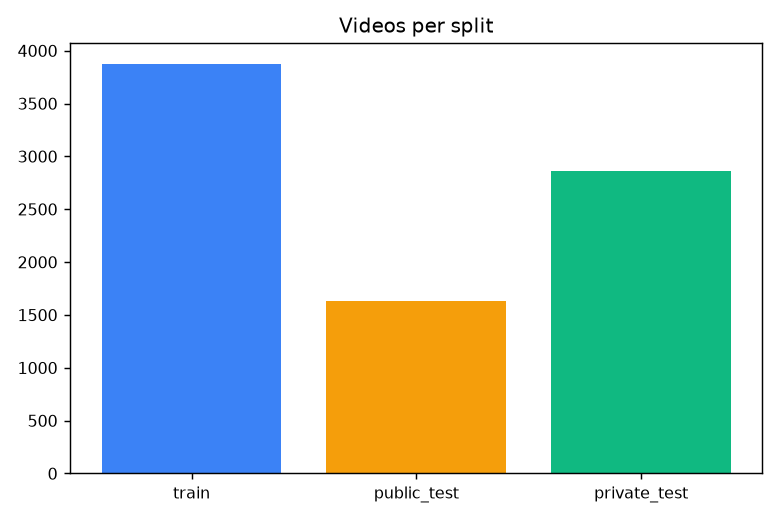
\includegraphics[width=0.6\textwidth]{split_sizes.png}
  \caption{Số lượng video trong ba tập \texttt{train}, \texttt{public\_test} và \texttt{private\_test}.}
  \label{fig:eda_split_sizes}
\end{figure}

\paragraph{Định dạng video} Toàn bộ 8.364 tệp đều là \texttt{.mp4} và đọc được; không có video nào có 0 khung hình. Độ phân giải đồng nhất tuyệt đối: 100\% video ở cả ba tập đều là $224\times224$ (Bảng~\ref{tab:eda_res}). Số khung hình gần như cố định ở mức 30 (chi tiết ở Mục~\ref{subsec:eda_uni}).

\begin{table}[H]
  \centering
  \caption{Thống kê độ phân giải video.}
  \label{tab:eda_res}
  \begin{tabular}{@{}lrrr@{}}
    \toprule
    \textbf{Tập} & \textbf{Độ phân giải} & \textbf{Số video} & \textbf{Tỷ lệ} \\
    \midrule
    train         & $224\times224$ & 3.875 & 100\% \\
    public\_test  & $224\times224$ & 1.630 & 100\% \\
    private\_test & $224\times224$ & 2.859 & 100\% \\
    \bottomrule
  \end{tabular}
\end{table}

\paragraph{Quan sát trực quan} Để kiểm chứng bằng mắt, nhóm trích 6--8 khung hình phân bố đều trong video (\texttt{cap.set(cv2.CAP\_\allowbreak PROP\_\allowbreak POS\_\allowbreak FRAMES, i)} với $i$ lấy từ \texttt{np.linspace}) và ghép thành lưới ảnh cho một số lớp (Hình~\ref{fig:eda_samples}). Các video được quay chính diện, người ký ngồi hoặc đứng giữa khung hình, thấy rõ phần thân trên, hai tay và khuôn mặt; nền chủ yếu là tường trơn với ánh sáng trong nhà. Sự đa dạng nằm ở người ký (giới tính, trang phục, kính), màu nền (be, xanh nhạt, trắng) và vị trí tay lúc bắt đầu. Ký hiệu thường chỉ chiếm một phần thời lượng: các khung đầu và cuối thường là tư thế nghỉ. Ở một số video xuất hiện các khung \emph{đơn sắc hoàn toàn} (hàng \textit{Phỏng vấn}, \textit{Uống}); hiện tượng này được định lượng ở Mục~\ref{subsec:eda_quality}.

\begin{figure}[H]
  \centering
  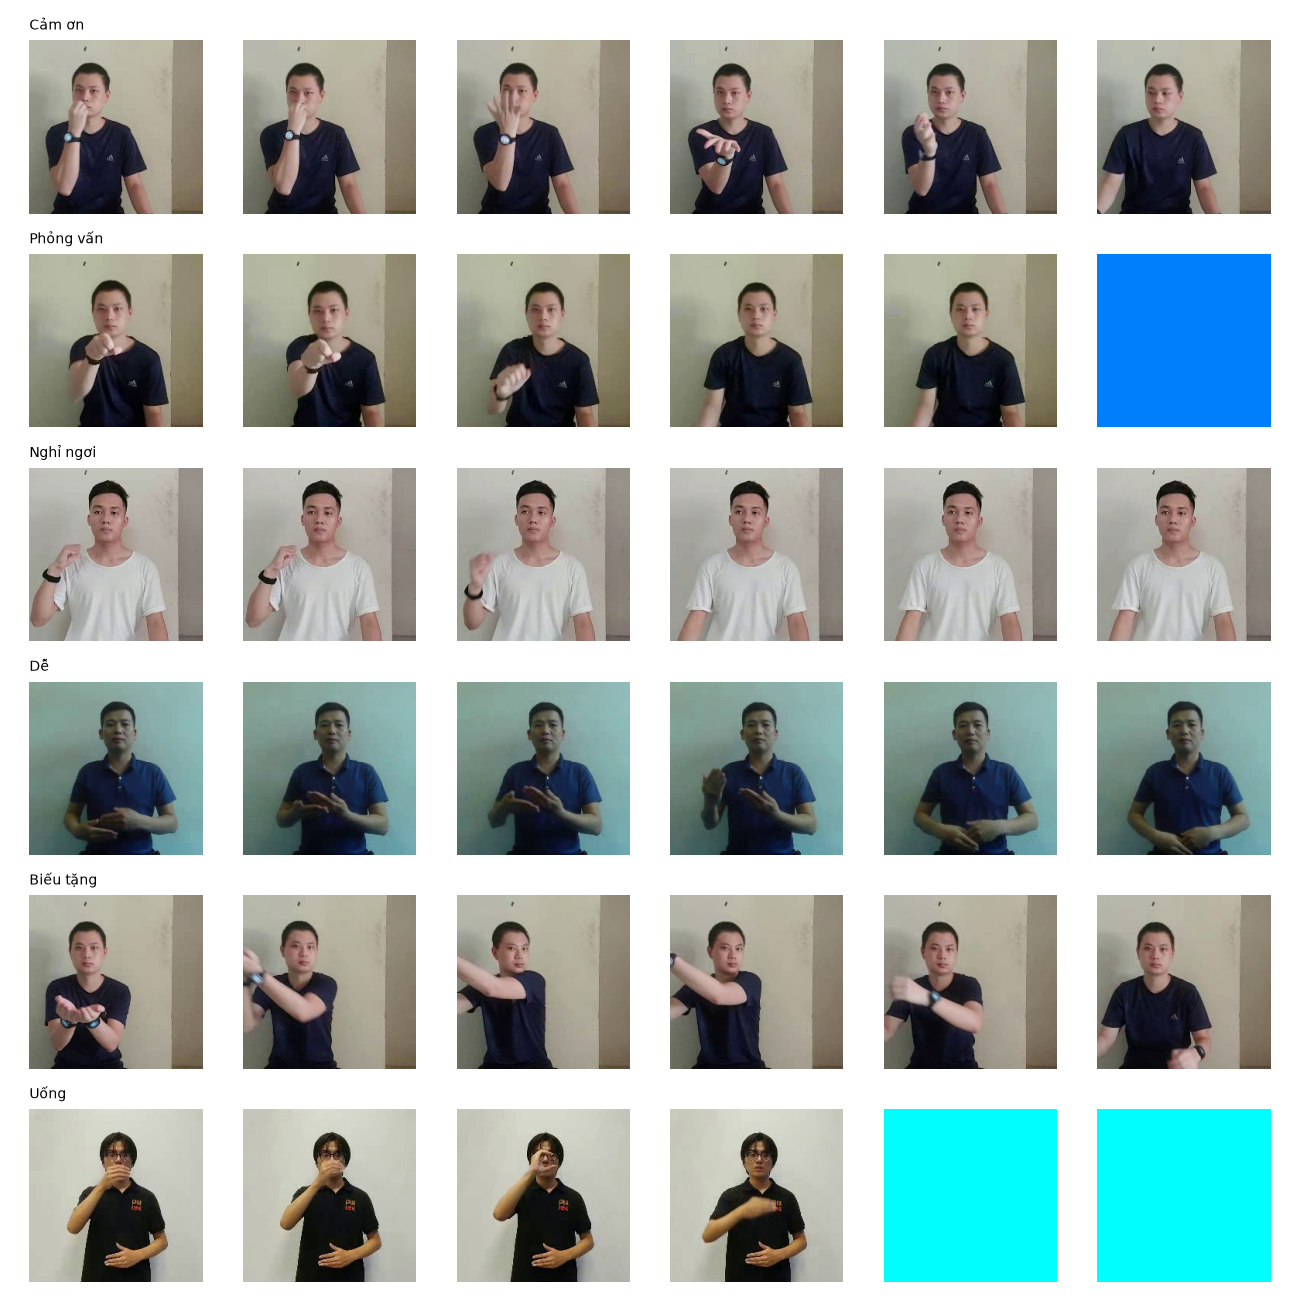
\includegraphics[width=0.85\textwidth]{sample_frames_6classes.png}
  \caption{Khung hình mẫu (lấy đều theo thời gian) của sáu lớp. Hàng \textit{Phỏng vấn} và \textit{Uống} có các khung đơn sắc ở cuối video.}
  \label{fig:eda_samples}
\end{figure}

\noindent\textit{Hệ quả:} khi gán nhãn số cho video phải chuẩn hoá tên lớp bằng \texttt{unicodedata.normalize(\textquotesingle NFC\textquotesingle, ...)} trước khi tra \texttt{label\_mapping.pkl}, nếu không phần lớn video sẽ không tìm được nhãn. Chỉ có tập \texttt{train} mang nhãn nên tập kiểm định (\textit{validation}) phải tách ra từ chính tập này; việc tách cần tính đến trùng lặp (Mục~\ref{subsec:eda_quality}). Thông tin phân biệt nằm ở hình dạng và chuyển động của bàn tay, khẩu hình và tư thế, nên các phép tăng cường không được làm đổi ngữ nghĩa không gian; đặc biệt \emph{không} dùng lật ngang (\textit{Horizontal Flip}) vì có thể đổi nghĩa tay trái/phải.

% =====================================================================
\subsubsection{Chất lượng dữ liệu}
\label{subsec:eda_quality}

\paragraph{Script và cách thực hiện}
\begin{itemize}
  \item \textbf{Script:} bốn script trong \texttt{02\_data\_quality/}, chạy theo thứ tự: \edafile{02\_data\_quality}{01\_integrity\_missing.py}, \edafile{02\_data\_quality}{02\_duplicates.py}, \edafile{02\_data\_quality}{03\_frame\_scan.py}, \edafile{02\_data\_quality}{04\_frame\_quality\_summary.py}. Kiểm tra bằng mắt dùng \edafile{07\_visual\_inspection}{02\_flagged\_videos.py}.
  \item \textbf{Cách khai thác dữ liệu:} 
  
  (i) \emph{Giá trị thiếu và lỗi đọc:} \texttt{01\_integrity\_missing.py} đếm ô trống (\texttt{isna}) theo cột và theo tập, đếm video có 0 khung, FPS hoặc kích thước bằng 0, rồi liệt kê các tệp có giá trị phi lý theo ngưỡng tuyệt đối (dưới 10~KB, dưới 16 khung, FPS dưới 5). 
  
  (ii) \emph{Trùng lặp:} \texttt{02\_duplicates.py} đọc toàn bộ byte của từng tệp, tính \texttt{hashlib.md5} một lần và lưu vào \texttt{file\_hashes.csv}; hai tệp cùng mã băm là cùng nội dung. Gom nhóm theo mã băm để đếm bản sao, tìm nhóm có nhiều hơn một nhãn (xung đột nhãn), lấy giao các tập mã băm giữa train, public test, private test, rồi giữ một tệp cho mỗi mã băm và đếm lại số video mỗi lớp. 
  
  (iii) \emph{Khung đơn sắc:} \texttt{03\_frame\_scan.py} giải mã \emph{từng} khung bằng \texttt{cap.read()}, tính độ lệch chuẩn điểm ảnh của từng kênh màu và coi khung là đơn sắc khi giá trị lớn nhất nhỏ hơn 3; đồng thời đếm số khung đơn sắc liên tiếp ở đầu video và tính độ chuyển động là trung bình $|f_t-f_{t-1}|$ trên ảnh xám. \texttt{04\_frame\_quality\_summary.py} đối chiếu số khung đọc được với metadata, bỏ các bản sao \texttt{\_N}, phân loại vị trí khung đơn sắc (đầu, cuối, giữa, toàn bộ) và mô phỏng việc lấy $T=16$ khung bằng \texttt{np.linspace} để đếm số khung đơn sắc bị lấy trúng. 
  
  (iv) \emph{Kiểm tra bằng mắt:} \texttt{02\_flagged\_videos.py} \emph{tự chọn} video cần xem từ kết quả hai bước trên, không dùng danh sách chọn tay. Tiêu chí chọn gồm: 6 video có tỷ lệ khung đơn sắc cao nhất trong số các video có từ 50\% khung đơn sắc trở lên; mọi video thuộc nhóm MD5 nằm ở hơn một lớp; một ví dụ cho mỗi dạng xuất hiện khung đơn sắc. Ngoại lai theo quy tắc Tukey được tính ở bước đơn biến (Mục~\ref{subsec:eda_uni}).
  \item \textbf{Đầu ra:} \texttt{integrity\_summary.txt}, \texttt{file\_hashes.csv}, \texttt{dups\_summary.txt}, \texttt{dedup\_summary.txt}, \texttt{class\_counts\_train\_unique\_vs\_all.csv}, \texttt{video\_quality\_flags.csv}, \texttt{solid\_frame\_summary.txt}, \texttt{class\_solid\_frame\_ratio.csv}; ở bước kiểm tra bằng mắt là \texttt{flagged\_videos\_info.txt}, \texttt{flagged\_videos\_check.png}, \texttt{solid\_frame\_patterns.png}.
\end{itemize}

Nhóm kiểm tra chất lượng dữ liệu theo các khía cạnh: giá trị thiếu, bản ghi trùng lặp, khung hình đơn sắc/video rỗng, giá trị ngoại lai, nhiễu nhãn và trùng lặp giữa các tập. Bảng~\ref{tab:eda_quality} tóm tắt các vấn đề phát hiện được.

\begin{table}[H]
  \centering
  \caption{Tóm tắt các vấn đề chất lượng dữ liệu.}
  \label{tab:eda_quality}
  \small
  \begin{tabular}{@{}p{0.26\textwidth}p{0.36\textwidth}p{0.30\textwidth}@{}}
    \toprule
    \textbf{Vấn đề} & \textbf{Số lượng} & \textbf{Ví dụ} \\
    \midrule
    Bản sao hậu tố \texttt{\_N} trong train & 1.069 tệp giống hệt bản gốc; còn 2.776 video duy nhất & \texttt{127824.mp4}, \texttt{127824\_1.mp4}, \texttt{127824\_2.mp4} \\
    Video có khung đơn sắc (train) & 758/3.875 tệp; 565/2.776 video duy nhất (20,4\%), ở 78/100 lớp & \texttt{Thất lạc/708519}, \texttt{Bộ y tế/523389} \\
    Video rỗng hoàn toàn & 2 video gốc (4 tệp kể cả bản sao) & \texttt{Biết/214576}, \texttt{Khai báo/885339} \\
    Nhiễu nhãn (cùng nội dung, khác lớp) & 2 nhóm nội dung, 5 tệp & \textit{Chậm lại} $\leftrightarrow$ \textit{Chào} \\
    Trùng train $\rightarrow$ public test & 157 video public giống hệt video train & -- \\
    Trùng public $\leftrightarrow$ private & 896 video & -- \\
    \bottomrule
  \end{tabular}
\end{table}

\paragraph{Giá trị thiếu và lỗi đọc} Bảng metadata không có giá trị thiếu ở bất kỳ thuộc tính nào (nhãn \texttt{cls} chỉ trống ở hai tập test vì các tập này vốn không có nhãn). Mọi video đều mở và giải mã được, và ở cả 8.364 video, số khung giải mã thực tế khớp với số khung ghi trong metadata. Như vậy không có vấn đề về tệp hỏng hay nhãn bị thiếu ở tập train.

\paragraph{Trùng lặp trong tập train} Nhóm tính mã băm MD5 nội dung từng tệp (\texttt{hashlib.md5}) rồi gom nhóm theo mã băm. Có 1.069/3.875 tệp mang hậu tố \texttt{\_1}, \texttt{\_2}, \texttt{\_3}\ldots{} So sánh từng cặp cho thấy cả 1.069 tệp này đều có bản gốc tồn tại, cùng lớp và \emph{giống hệt bản gốc từng byte} (cùng số khung, FPS, dung lượng): đây là bản sao, không phải biến thể tăng cường. Có 176 video gốc có 1 bản sao, 169 video có 2 và 185 video có 3. Tính cả các bản sao khác, tập train có 1.099 tệp dư thừa và chỉ còn \textbf{2.776 video duy nhất}. Các bản sao tập trung ở những lớp vốn đã nhiều mẫu (\textit{Chậm lại} và \textit{Trường học} cùng thêm 25 tệp, \textit{Rau} và \textit{Nhìn} thêm 23, \textit{Khóc} thêm 22\ldots), nên sau khi khử trùng lặp số video mỗi lớp còn từ 5 đến 51 (trung bình 27,8; tỷ lệ chênh $\approx$10,2 lần). Bảng trước/sau khử trùng lặp của từng lớp lưu ở \texttt{class\_counts\_train\_unique\_vs\_all.csv}. Hệ quả là nguy cơ rò rỉ dữ liệu (\textit{Data Leakage}): nếu chia train/validation ngẫu nhiên theo từng tệp, các bản sao của cùng một video rơi vào cả hai phần, làm điểm validation bị thổi phồng.

\paragraph{Khung hình đơn sắc và video rỗng} Nhóm đọc \emph{toàn bộ} khung hình của 8.364 video và tính độ lệch chuẩn giá trị điểm ảnh trên từng kênh màu; khung có độ lệch chuẩn lớn nhất giữa ba kênh nhỏ hơn 3 được coi là \emph{khung đơn sắc}. Kết quả tổng hợp ở Bảng~\ref{tab:eda_solid}.

\begin{table}[H]
  \centering
  \caption{Số video chứa khung hình đơn sắc theo từng tập.}
  \label{tab:eda_solid}
  \begin{tabular}{@{}lrrrr@{}}
    \toprule
    \textbf{Tập} & \textbf{Tổng video} & \textbf{Có $\geq$1 khung đơn sắc} & \textbf{Đơn sắc toàn bộ} & \textbf{Tỷ lệ} \\
    \midrule
    train (tất cả tệp)        & 3.875 & 758 & 4 & 19,6\% \\
    train (video duy nhất)    & 2.776 & 565 & 2 & 20,4\% \\
    public\_test              & 1.630 & 1   & 0 & 0,06\% \\
    private\_test             & 2.859 & 1   & 0 & 0,03\% \\
    \bottomrule
  \end{tabular}
\end{table}

Đây là phát hiện đáng chú ý nhất của EDA. Khoảng một phần năm số video duy nhất trong train (565/2.776, thuộc 78/100 lớp) chứa khung đơn sắc, và số khung này không nhỏ: trung bình 12,2 khung trên khoảng 30 khung mỗi video (trung vị 12, nhiều nhất 23). Các khung có màu thuần (đỏ, xanh lục, xanh lam, xanh lục lam, tím, vàng, trắng, đen, xám) và xuất hiện theo các dạng: chỉ ở đầu video (231 video), chỉ ở cuối (161), cả đầu và cuối (116), xen ở giữa (55) hoặc toàn bộ video (2) (Hình~\ref{fig:eda_solid_examples}). Lớp có tỷ lệ video bị ảnh hưởng cao nhất là \textit{Có thể} (6/15 video duy nhất), \textit{Xin lỗi} (5/14) và \textit{Thất lạc} (7/20) (chi tiết ở \texttt{class\_solid\_frame\_ratio.csv}).

\begin{figure}[H]
  \centering
  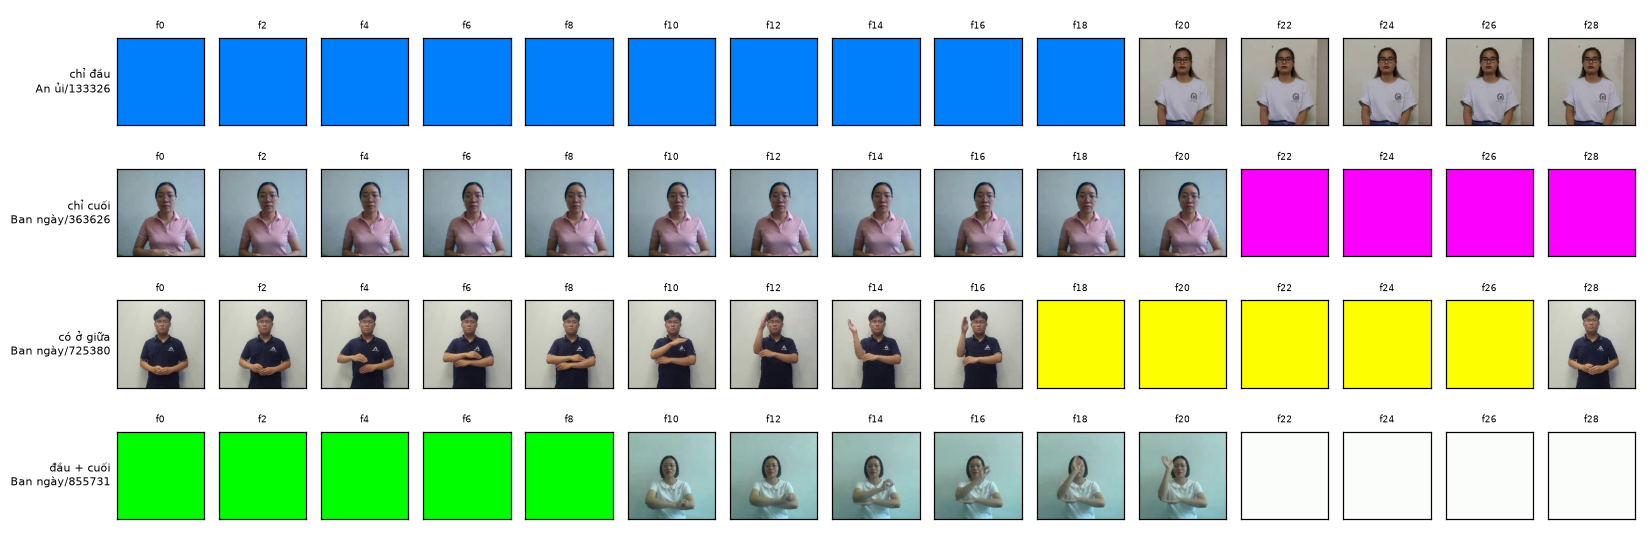
\includegraphics[width=\textwidth]{solid_frame_patterns.png}
  \caption{Bốn dạng khung đơn sắc trong tập train (khung chẵn $f_0$--$f_{28}$), mỗi dạng một video được chọn tự động: chỉ ở đầu (\textit{An ủi}/133326), chỉ ở cuối (\textit{Ban ngày}/363626), xen ở giữa (\textit{Ban ngày}/725380), cả đầu và cuối (\textit{Ban ngày}/855731).}
  \label{fig:eda_solid_examples}
\end{figure}

Hiện tượng này ảnh hưởng trực tiếp đến cách lấy mẫu: khi lấy $T=16$ khung đều nhau bằng \texttt{linspace} trên 565 video nói trên, trung bình có 6,4/16 khung được chọn là khung đơn sắc, và ở 224 video có từ 8/16 khung trở lên (ít nhất một nửa chuỗi đầu vào) là khung đơn sắc. Ngược lại, mỗi tập test chỉ có 1 video chứa đúng 1 khung đơn sắc. Như vậy khung đơn sắc là đặc điểm \emph{riêng của tập train}: nếu không xử lý, mô hình vừa mất thông tin ký hiệu, vừa có thể học các tín hiệu giả không tồn tại ở dữ liệu kiểm tra.

Sáu hàng đầu của Hình~\ref{fig:eda_suspicious} là các video có tỷ lệ khung đơn sắc cao nhất. Hai video được xác nhận bằng mắt là \textbf{rỗng hoàn toàn}: \texttt{Biết/214576.mp4} (2,5~KB, 16 khung, toàn màu xanh lục) và \texttt{Khai báo/885339.mp4} (2,7~KB, 23 khung, toàn màu xanh lam, kèm 2 bản sao \texttt{\_1}, \texttt{\_2}); cả hai không có người ký. Bốn video tiếp theo có 20--21/30 khung đơn sắc: \texttt{Nôn ói/915809}, \texttt{Thất lạc/708519}, \texttt{Chân/984642} và \texttt{Khai báo/362529}. Người ký chỉ xuất hiện trong khoảng 10 khung, ví dụ \texttt{Khai báo/362529} có 20 khung đỏ đầu tiên ($f_0$--$f_{19}$).

\paragraph{Giá trị ngoại lai} Nhóm dùng quy tắc Tukey (ngoài khoảng $[Q_1-1{,}5\,\mathrm{IQR},\,Q_3+1{,}5\,\mathrm{IQR}]$ tính trên tập train) cho thời lượng, dung lượng và FPS. Số lượng ngoại lai khá nhiều nhưng phần lớn chỉ lệch nhẹ (Mục~\ref{subsec:eda_uni}). Đáng chú ý là các ngoại lai cực đoan: thời lượng trên 5~s có 10 video train, 1 video public test và 3 video private test (lớn nhất 35,3~s ở train, 28,1~s ở private test); FPS dưới 5 có 9 video train và 2 video private test; dung lượng dưới 10~KB có 4 tệp train, đều là các video rỗng nói trên. Các ngoại lai này không nhất thiết là lỗi mà phản ánh việc video được lấy mẫu lại về $\approx$30 khung từ các clip gốc có độ dài rất khác nhau.

\paragraph{Nhiễu nhãn} Khi gom nhóm theo MD5, có hai nhóm nội dung giống hệt nhau nhưng nằm ở \emph{hai lớp khác nhau}: \texttt{Chậm lại/284430.mp4} trùng với \texttt{Chào/392683.mp4} và \texttt{Chào/468203.mp4}; \texttt{Chậm lại/254739.mp4} trùng với \texttt{Chào/792094.mp4}. Nhóm đã xem trực tiếp (Hình~\ref{fig:eda_suspicious}, năm hàng cuối) và xác nhận chúng có cùng người ký, cùng chuỗi động tác. Một video không thể đồng thời mang hai nghĩa nên ít nhất một trong hai nhãn là sai; tuy nhiên việc xác định nhãn đúng cần người am hiểu ngôn ngữ ký hiệu Việt Nam, nên báo cáo chỉ ghi nhận đây là \emph{xung đột nhãn}.

\begin{figure}[H]
  \centering
  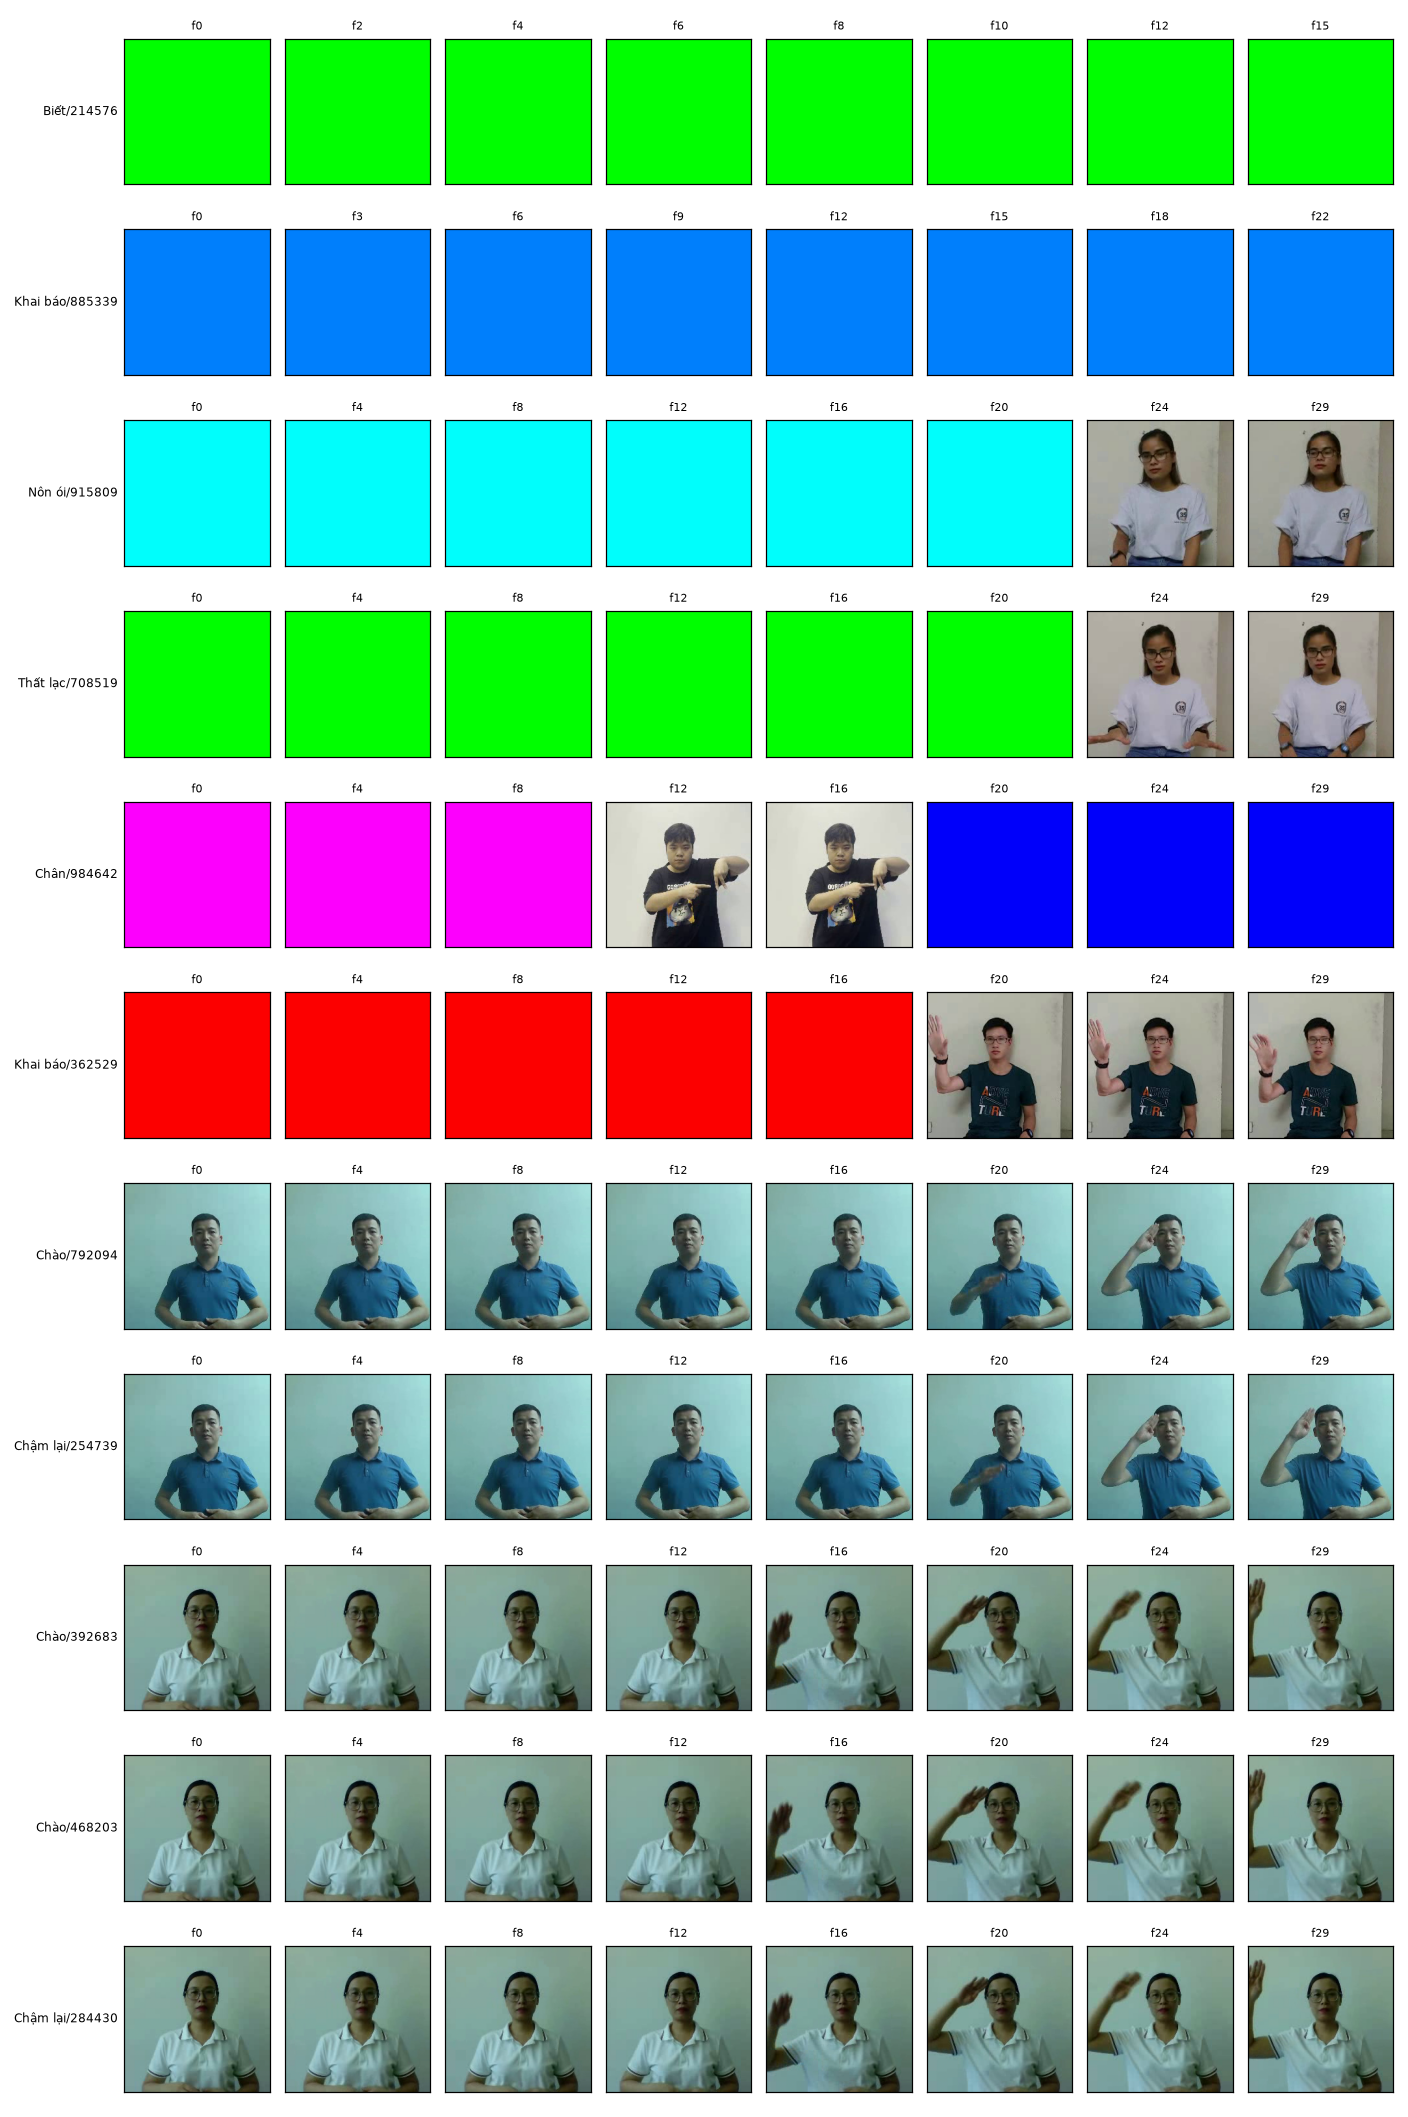
\includegraphics[width=0.9\textwidth,height=0.72\textheight,keepaspectratio]{flagged_videos_check.png}
  \caption{Kiểm tra bằng mắt các video do bước kiểm tra chất lượng tự đánh dấu. Sáu hàng đầu là các video có tỷ lệ khung đơn sắc cao nhất, gồm hai video rỗng hoàn toàn (\textit{Biết}/214576, \textit{Khai báo}/885339). Năm hàng cuối là hai nhóm video trùng nội dung nhưng khác nhãn (\textit{Chậm lại} $\leftrightarrow$ \textit{Chào}).}
  \label{fig:eda_suspicious}
\end{figure}

\paragraph{Trùng lặp giữa các tập} Public test có 8 bản trùng nội bộ (1.622 video duy nhất) và \textbf{157 video giống hệt video trong train}; private test có 2.782 video duy nhất, không trùng với train, nhưng có 896 video trùng với public test. Ngoài ra, 2.806 tên tệp trong private test trùng với tên tệp trong train nhưng nội dung hoàn toàn khác (MD5 khác, chênh lệch điểm ảnh lớn), nên đây chỉ là trùng cách đặt mã số; nguyên nhân chưa rõ và tên tệp \emph{không} được dùng để suy luận nhãn.

\noindent\textit{Hệ quả:} dữ liệu train chưa sạch; trước khi huấn luyện cần khử trùng lặp, loại video rỗng, xử lý khung đơn sắc và rà soát các nhãn xung đột. Điểm trên public test có thể bị ảnh hưởng một phần bởi 157 video đã có trong train.

% =====================================================================
\subsubsection{Phân tích đơn biến}
\label{subsec:eda_uni}

\paragraph{Script và cách thực hiện}
\begin{itemize}
  \item \textbf{Script:} \edafile{03\_univariate}{01\_numeric\_attributes.py}.
  \item \textbf{Cách khai thác dữ liệu:} với mỗi thuộc tính số (\texttt{frames}, \texttt{fps}, \texttt{dur}, \texttt{size\_kb}), script tính \texttt{groupby(\textquotesingle split\textquotesingle).describe()} (trung bình, độ lệch chuẩn, min, các tứ phân vị, max), hệ số lệch (\textit{skewness}) và các giá trị phổ biến nhất. Ngoại lai được xác định theo quy tắc Tukey với ngưỡng tính trên train rồi áp lên cả ba tập. Script vẽ histogram của từng thuộc tính cho ba tập trên cùng trục; histogram FPS và dung lượng dùng mật độ (\texttt{density=True}) để so sánh được các tập có kích thước khác nhau.
  \item \textbf{Đầu ra:} \texttt{desc\_by\_split.csv} (Bảng~\ref{tab:eda_desc}), \texttt{univariate\_summary.txt}, \texttt{frames\_hist\_by\_split.png}, \texttt{fps\_hist\_by\_split.png}, \texttt{filesize\_hist\_by\_split.png}.
\end{itemize}

Mục này khảo sát phân phối của từng thuộc tính số: số khung hình, FPS, thời lượng và dung lượng, tính trên từng tập (Bảng~\ref{tab:eda_desc}). Độ phân giải đã được trình bày ở Bảng~\ref{tab:eda_res}.

\begin{table}[H]
  \centering
  \caption{Thống kê mô tả các thuộc tính số theo từng tập.}
  \label{tab:eda_desc}
  \small
  \begin{tabular}{@{}llrrrrrrr@{}}
    \toprule
    \textbf{Thuộc tính} & \textbf{Tập} & \textbf{Mean} & \textbf{Std} & \textbf{Min} & \textbf{Q1} & \textbf{Median} & \textbf{Q3} & \textbf{Max} \\
    \midrule
    \multirow{3}{*}{Số khung}
      & train   & 29,88 & 1,26 & 16 & 30 & 30 & 30 & 30 \\
      & public  & 29,96 & 0,66 & 16 & 30 & 30 & 30 & 30 \\
      & private & 29,98 & 0,44 & 21 & 30 & 30 & 30 & 30 \\
    \midrule
    \multirow{3}{*}{FPS}
      & train   & 12,94 & 3,11 & 0,85 & 10,98 & 12,34 & 14,06 & 30,02 \\
      & public  & 12,97 & 3,00 & 5,93 & 10,98 & 12,50 & 13,85 & 30,00 \\
      & private & 13,32 & 3,69 & 1,07 & 10,84 & 12,50 & 14,06 & 30,02 \\
    \midrule
    \multirow{3}{*}{Thời lượng (s)}
      & train   & 2,48 & 1,36 & 0,70 & 2,13 & 2,43 & 2,73 & 35,29 \\
      & public  & 2,42 & 0,51 & 0,70 & 2,17 & 2,40 & 2,73 & 5,06 \\
      & private & 2,42 & 0,82 & 0,70 & 2,13 & 2,40 & 2,77 & 28,14 \\
    \midrule
    \multirow{3}{*}{Dung lượng (KB)}
      & train   & 85,5  & 38,5 & 2,5  & 60,2 & 80,6 & 103,0 & 263,8 \\
      & public  & 113,6 & 77,5 & 26,2 & 76,1 & 91,0 & 125,8 & 483,2 \\
      & private & 116,3 & 77,7 & 42,2 & 77,7 & 94,6 & 126,0 & 488,0 \\
    \bottomrule
  \end{tabular}
\end{table}

\paragraph{Số khung hình} Hầu hết video có đúng 30 khung: 3.832/3.875 video train (98,9\%), 1.623/1.630 public test và 2.850/2.859 private test; ở train có 26 video chỉ có 16 khung. Không video nào ngắn hơn 16 khung (Hình~\ref{fig:eda_frames_hist}), nên không cần đệm khung thực sự khi lấy $T=16$.

\begin{figure}[H]
  \centering
  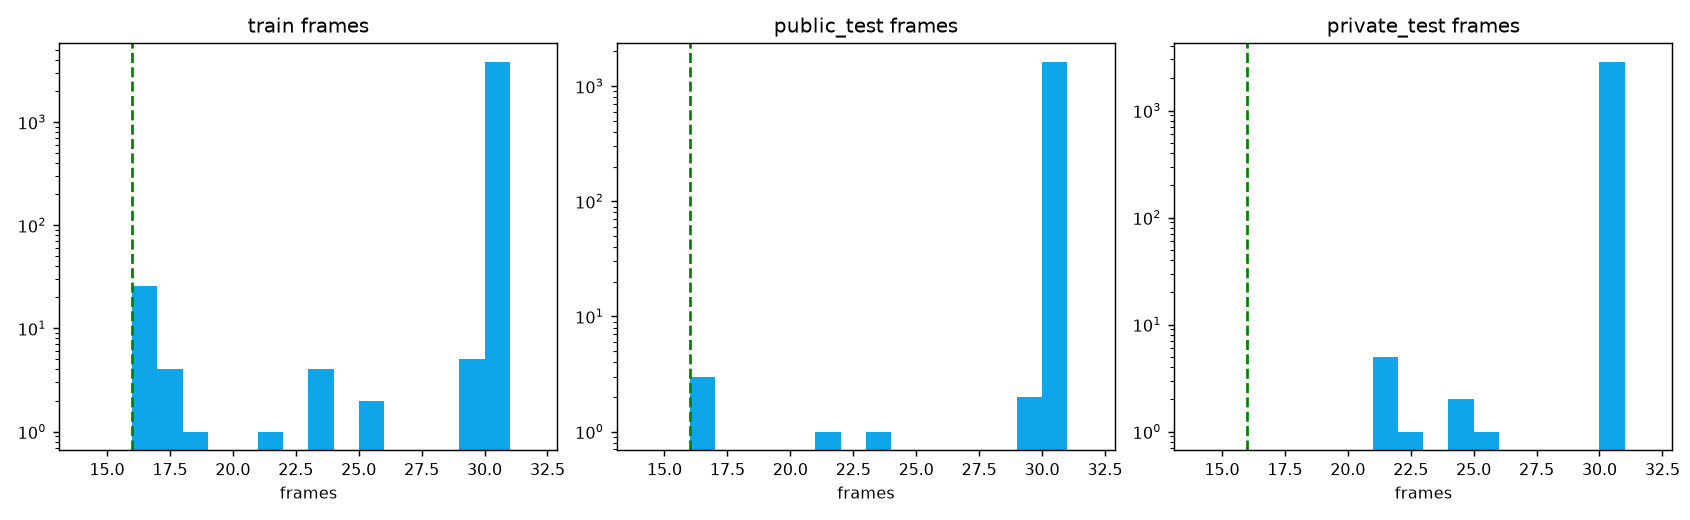
\includegraphics[width=\textwidth]{frames_hist_by_split.png}
  \caption{Histogram số khung hình mỗi video theo tập (trục tung thang log). Đường đứt nét đánh dấu $T=16$.}
  \label{fig:eda_frames_hist}
\end{figure}

\paragraph{FPS và thời lượng} Dù số khung gần như cố định, FPS biến thiên mạnh: train có 961 giá trị FPS khác nhau, từ 0,85 đến 30,02 (trung vị 12,3), phân phối lệch phải với đuôi dài (hệ số lệch 1,01 ở train; Hình~\ref{fig:eda_fps_hist}). Vì thời lượng $=\texttt{frames}/\texttt{fps}$ nên thời lượng thực của cùng 30 khung dao động lớn: trung vị khoảng 2,4~s nhưng có video tới 35,3~s ở train và 28,1~s ở private test, trong khi 99\% video đều ngắn hơn khoảng 4~s. Điều này cho thấy video đã được lấy mẫu lại về khoảng 30 khung bất kể độ dài clip gốc.

\begin{figure}[H]
  \centering
  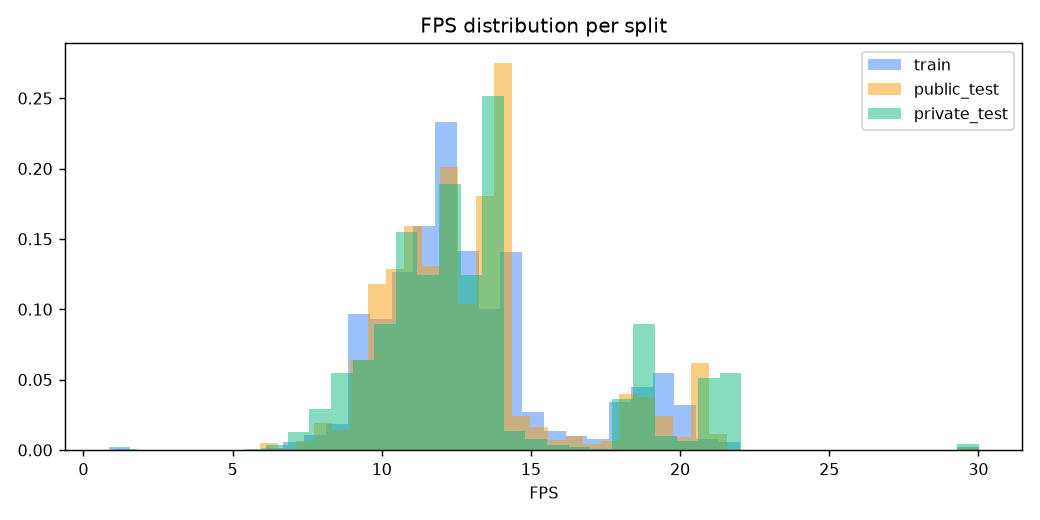
\includegraphics[width=0.85\textwidth]{fps_hist_by_split.png}
  \caption{Phân phối FPS theo từng tập.}
  \label{fig:eda_fps_hist}
\end{figure}

\paragraph{Dung lượng tệp} Dung lượng train có trung vị 80,6~KB (trung bình 85,5; từ 2,5 đến 263,8~KB). Hai tập test có phân phối lệch phải hơn hẳn: trung bình 113,6--116,3~KB, lớn nhất tới 483--488~KB (Hình~\ref{fig:eda_size_hist}); khác biệt này được phân tích ở Mục~\ref{subsec:eda_shift}.

\begin{figure}[H]
  \centering
  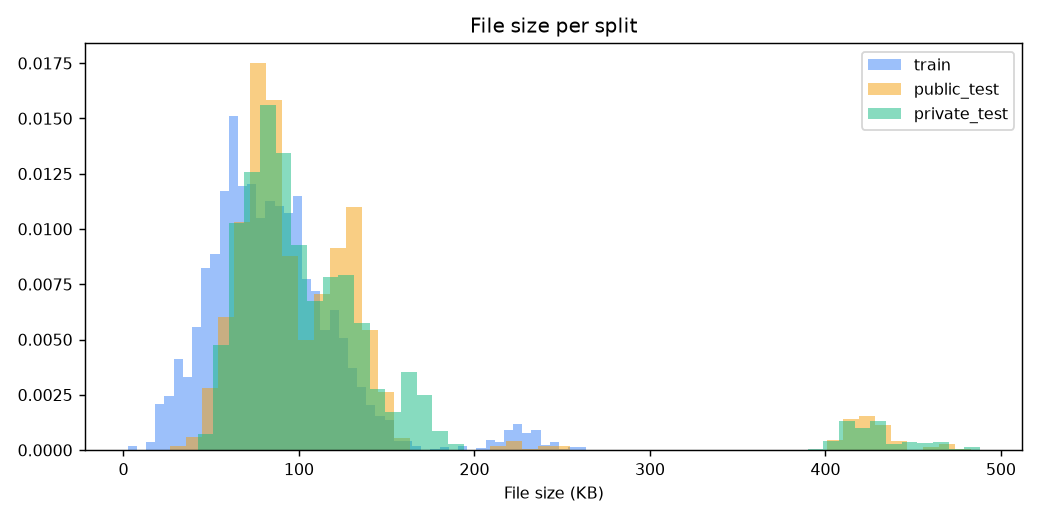
\includegraphics[width=0.85\textwidth]{filesize_hist_by_split.png}
  \caption{Phân phối dung lượng tệp (KB) theo từng tập.}
  \label{fig:eda_size_hist}
\end{figure}

\noindent\textit{Hệ quả:} (i) không cần đổi kích thước khung hình, tuy kiến trúc CRNN với \texttt{Adaptive\allowbreak AvgPool2d} vẫn đảm bảo tính tổng quát nếu gặp video khác độ phân giải; (ii) vì mọi video có ít nhất 16 khung, lấy mẫu $T=16$ khung đều nhau bằng \texttt{linspace} (\textit{Frame Downsampling}) là đủ, lặp khung (\textit{repeat padding}) chỉ giữ làm phương án dự phòng; (iii) phân phối FPS và dung lượng lệch phải với nhiều ngoại lai nên nên dùng trung vị thay vì trung bình khi mô tả.

% =====================================================================
\subsubsection{Phân tích biến mục tiêu}
\label{subsec:eda_class}

\paragraph{Script và cách thực hiện}
\begin{itemize}
  \item \textbf{Script:} \edafile{04\_target\_analysis}{01\_class\_distribution.py}.
  \item \textbf{Cách khai thác dữ liệu:} lọc các dòng của tập train trong \texttt{video\_metadata.csv}, đếm số video mỗi nhãn bằng \texttt{value\_counts()}, sau đó tính trung bình, trung vị, độ lệch chuẩn, tỷ lệ lớp lớn nhất/nhỏ nhất và số lớp có không quá 25 hoặc từ 50 video trở lên. Số video mỗi lớp sau khử trùng lặp lấy từ \texttt{class\_counts\_train\_unique\_vs\_all.csv} của bước \texttt{02\_data\_quality}.
  \item \textbf{Đầu ra:} \texttt{class\_summary.txt}, \texttt{class\_counts\_train.csv}, \texttt{class\_distribution\_all.png}, \texttt{class\_top\_bottom10.png}, \texttt{samples\_per\_class\_hist.png}.
\end{itemize}

Nhóm dùng \texttt{value\_counts()} trên cột nhãn của tập \texttt{train} để đếm số video mỗi lớp, rồi vẽ biểu đồ cho cả 100 lớp (Hình~\ref{fig:eda_class_dist}), 10 lớp nhiều nhất/ít nhất (Hình~\ref{fig:eda_top_bottom}) và histogram số video mỗi lớp (Hình~\ref{fig:eda_spc_hist}).

\begin{figure}[H]
  \centering
  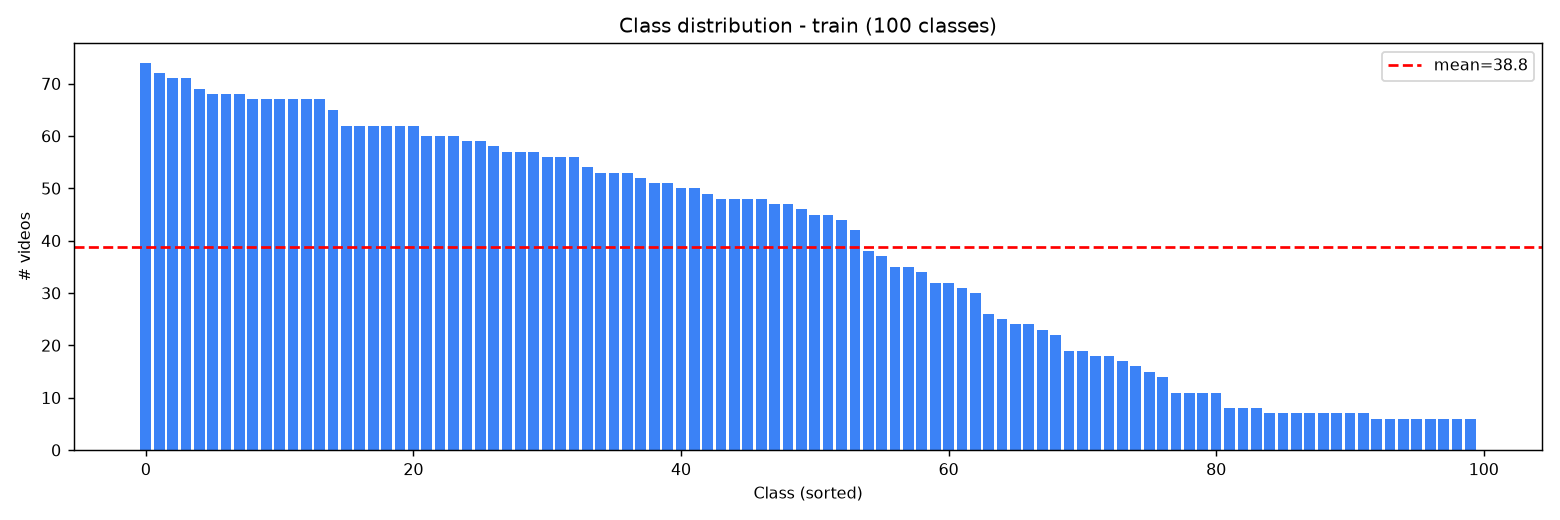
\includegraphics[width=\textwidth]{class_distribution_all.png}
  \caption{Phân phối số video theo lớp trong tập huấn luyện (100 lớp, sắp xếp giảm dần).}
  \label{fig:eda_class_dist}
\end{figure}

Tập huấn luyện gồm 3.875 video nhưng phân bố không đồng đều: trung bình 38,75 video/lớp, trung vị 45,5, độ lệch chuẩn 22,78. Lớp nhiều nhất (\textit{Trường học}) có 74 video, trong khi mười lớp chỉ có 6--7 video; tỷ lệ chênh giữa lớp lớn nhất và nhỏ nhất xấp xỉ $12{,}3$ lần (Bảng~\ref{tab:eda_top_bottom}). Có 36/100 lớp có không quá 25 video và 42/100 lớp có từ 50 video trở lên, tức phân phối có dạng hai đỉnh: nhóm lớp ``giàu'' (khoảng 45--74 video) và nhóm lớp ``nghèo'' (khoảng 6--11 video). Nhiều lớp ít mẫu thuộc nhóm từ vựng y tế -- dịch bệnh.

\begin{table}[H]
  \centering
  \caption{Mười lớp nhiều mẫu nhất và mười lớp ít mẫu nhất trong tập huấn luyện.}
  \label{tab:eda_top_bottom}
  \begin{tabular}{@{}lr@{\hspace{2.5em}}lr@{}}
    \toprule
    \multicolumn{2}{c}{\textbf{Nhiều nhất}} & \multicolumn{2}{c}{\textbf{Ít nhất}} \\
    \cmidrule(r){1-2}\cmidrule(l){3-4}
    \textbf{Lớp} & \textbf{Số video} & \textbf{Lớp} & \textbf{Số video} \\
    \midrule
    Trường học & 74 & Nhầm      & 7 \\
    Rau        & 72 & Virus     & 7 \\
    Nhà        & 71 & Bệnh nhân & 6 \\
    Áp dụng    & 71 & Cách ly   & 6 \\
    Chậm lại   & 69 & Cơ thể    & 6 \\
    Cám dỗ     & 68 & Ho        & 6 \\
    Nghe       & 68 & Phục hồi  & 6 \\
    Nói xấu    & 68 & Sốt       & 6 \\
    Biết       & 67 & Xe máy    & 6 \\
    Chạy       & 67 & Ủng hộ    & 6 \\
    \bottomrule
  \end{tabular}
\end{table}

\begin{figure}[H]
  \centering
  \begin{minipage}{0.56\textwidth}
    \centering
    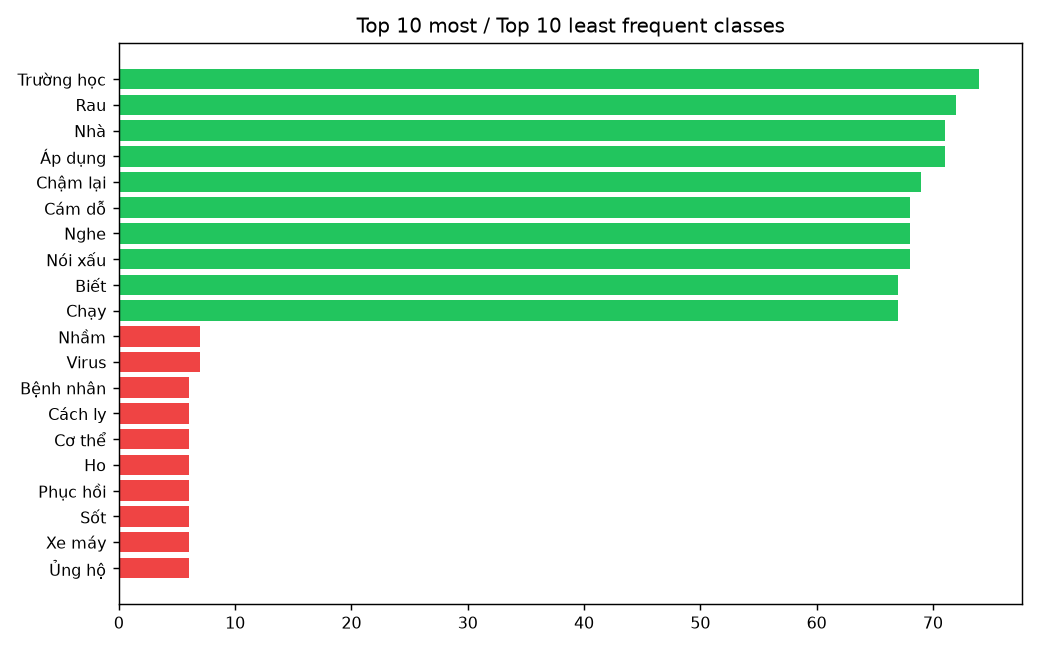
\includegraphics[width=\textwidth]{class_top_bottom10.png}
    \caption{Mười lớp nhiều nhất (xanh) và ít nhất (đỏ).}
    \label{fig:eda_top_bottom}
  \end{minipage}\hfill
  \begin{minipage}{0.42\textwidth}
    \centering
    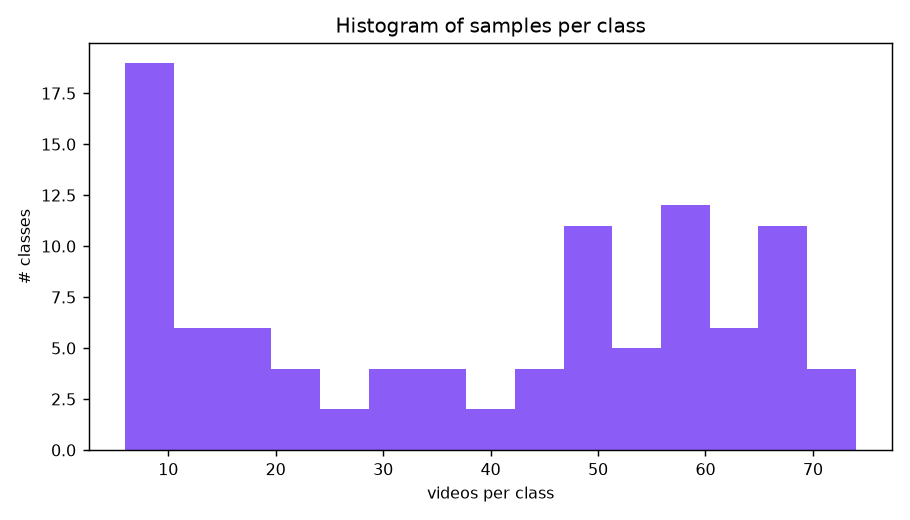
\includegraphics[width=\textwidth]{samples_per_class_hist.png}
    \caption{Histogram số video mỗi lớp.}
    \label{fig:eda_spc_hist}
  \end{minipage}
\end{figure}

Các con số trên tính trên tệp gốc, \emph{chưa} khử trùng lặp.

\noindent\textit{Hệ quả:} dữ liệu bị mất cân bằng lớp (\textit{Class Imbalance}) rõ rệt. Nếu đánh giá bằng Accuracy, mô hình có thể thiên về lớp phổ biến mà vẫn đạt điểm cao; vì vậy dùng Macro F1 (cũng là thước đo chính thức) và cần biện pháp xử lý mất cân bằng ở bước tiền xử lý/huấn luyện.

% =====================================================================
\subsubsection{Phân tích hai biến và đa biến}
\label{subsec:eda_multi}

\paragraph{Script và cách thực hiện}
\begin{itemize}
  \item \textbf{Script:} \edafile{05\_bivariate\_multivariate}{01\_correlation\_and\_label\_association.py}.
  \item \textbf{Cách khai thác dữ liệu:} ghép \texttt{video\_metadata.csv} với \texttt{video\_quality\_flags.csv} theo khoá (tập, lớp, tên tệp); bỏ các bản sao \texttt{\_N} để chỉ giữ 2.776 video duy nhất của train. Tính ma trận tương quan Pearson và Spearman (tương quan hạng, ít nhạy với ngoại lai) giữa các thuộc tính số; với từng thuộc tính, chia giá trị theo 100 lớp rồi chạy kiểm định Kruskal--Wallis (\texttt{scipy.stats.kruskal}) và tính $\eta^2 = SS_{\text{giữa lớp}}/SS_{\text{tổng}}$. Trung vị và tứ phân vị FPS của từng lớp được sắp xếp tăng dần để vẽ.
  \item \textbf{Đầu ra:} \texttt{multivariate\_summary.txt}, \texttt{corr\_heatmap.png}, \texttt{fps\_by\_class.png}, \texttt{size\_vs\_solid.png}.
\end{itemize}

Vì dữ liệu video không có đặc trưng dạng bảng, phân tích hai biến và đa biến tập trung vào mối quan hệ giữa các thuộc tính metadata với nhau và với nhãn lớp. Để tránh bản sao làm lệch kết quả, các phép tính dưới đây dùng 2.776 video duy nhất của tập train.

\paragraph{Tương quan giữa các thuộc tính} Hình~\ref{fig:eda_corr} cho thấy hệ số tương quan Pearson giữa số khung, FPS, dung lượng, tỷ lệ khung đơn sắc và độ chuyển động. (Thời lượng không đưa vào vì $\texttt{dur}=\texttt{frames}/\texttt{fps}$ nên phụ thuộc hoàn toàn vào hai biến còn lại.) Hầu hết các cặp có tương quan yếu ($|r|<0{,}35$); hai quan hệ rõ nhất là dung lượng -- tỷ lệ khung đơn sắc ($r\approx-0{,}45$; Spearman $\rho\approx-0{,}51$) và FPS -- chuyển động ($r\approx-0{,}34$; $\rho\approx-0{,}30$). Tương quan Spearman cho cùng chiều và độ lớn tương tự, nên các quan hệ này không phải do ngoại lai tạo ra. Quan hệ đầu là hợp lý: khung đơn sắc nén rất nhỏ nên video chứa nhiều khung đơn sắc có dung lượng thấp (Hình~\ref{fig:eda_size_solid}). Quan hệ sau cho thấy video có FPS thấp (clip gốc dài hơn) có độ chuyển động giữa các khung liên tiếp lớn hơn. Số khung gần như không liên quan tới các biến khác vì hầu như không đổi.

\begin{figure}[H]
  \centering
  \begin{minipage}{0.48\textwidth}
    \centering
    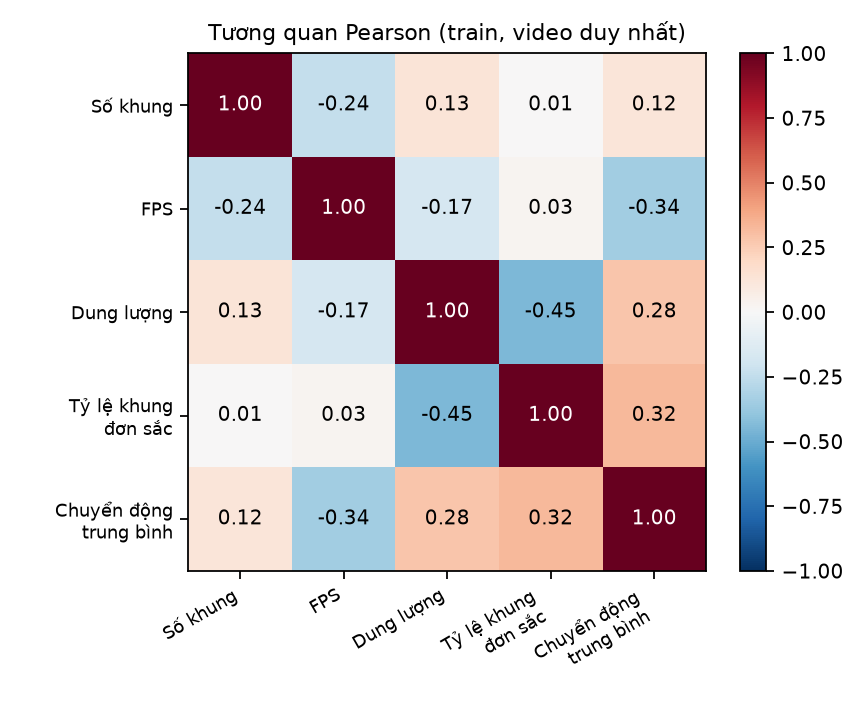
\includegraphics[width=\textwidth]{corr_heatmap.png}
    \caption{Ma trận tương quan Pearson giữa các thuộc tính (train, video duy nhất).}
    \label{fig:eda_corr}
  \end{minipage}\hfill
  \begin{minipage}{0.48\textwidth}
    \centering
    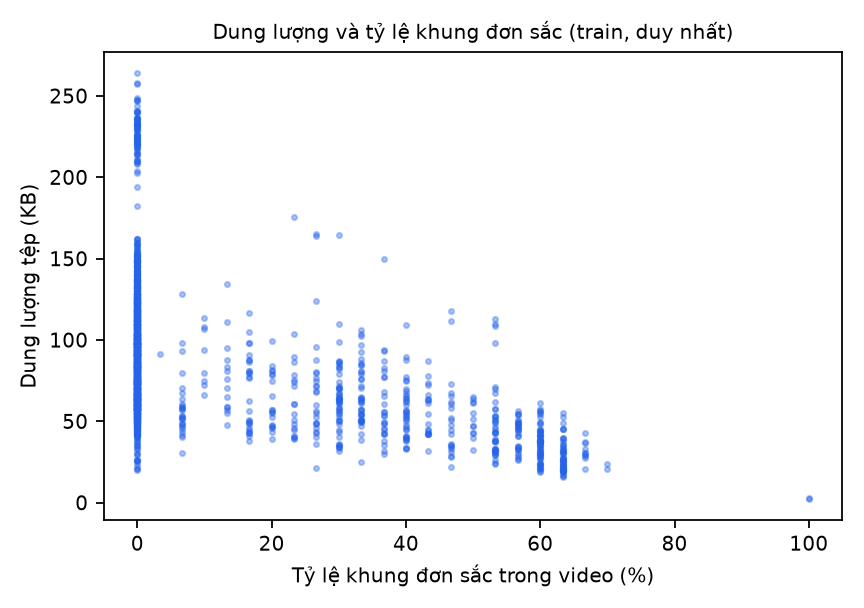
\includegraphics[width=\textwidth]{size_vs_solid.png}
    \caption{Dung lượng tệp theo tỷ lệ khung đơn sắc.}
    \label{fig:eda_size_solid}
  \end{minipage}
\end{figure}

\paragraph{Quan hệ giữa thuộc tính và nhãn lớp} Nhóm so sánh phân phối của từng thuộc tính giữa 100 lớp bằng kiểm định Kruskal--Wallis và hệ số $\eta^2$ (tỷ lệ phương sai giải thích bởi nhãn). Kết quả: FPS có $\eta^2\approx0{,}28$, dung lượng $\eta^2\approx0{,}15$, số khung $\eta^2\approx0{,}08$; cả ba đều có $p<10^{-10}$. Nói cách khác, FPS của video khác nhau rõ rệt giữa các lớp: trung vị FPS của lớp dao động từ khoảng 9,4 (\textit{Ngón tay}) đến khoảng 19,2 (\textit{Ho}), trong khi trung vị toàn tập là 12,4 (Hình~\ref{fig:eda_fps_class}). Điều này gợi ý rằng thời lượng clip gốc (và do đó FPS sau khi lấy mẫu lại) có liên hệ với từ được ký -- có thể vì các từ khác nhau có độ dài tự nhiên khác nhau -- hoặc vì cách thu thập dữ liệu theo từng lớp. Nhóm chưa xác định được nguyên nhân.

\begin{figure}[H]
  \centering
  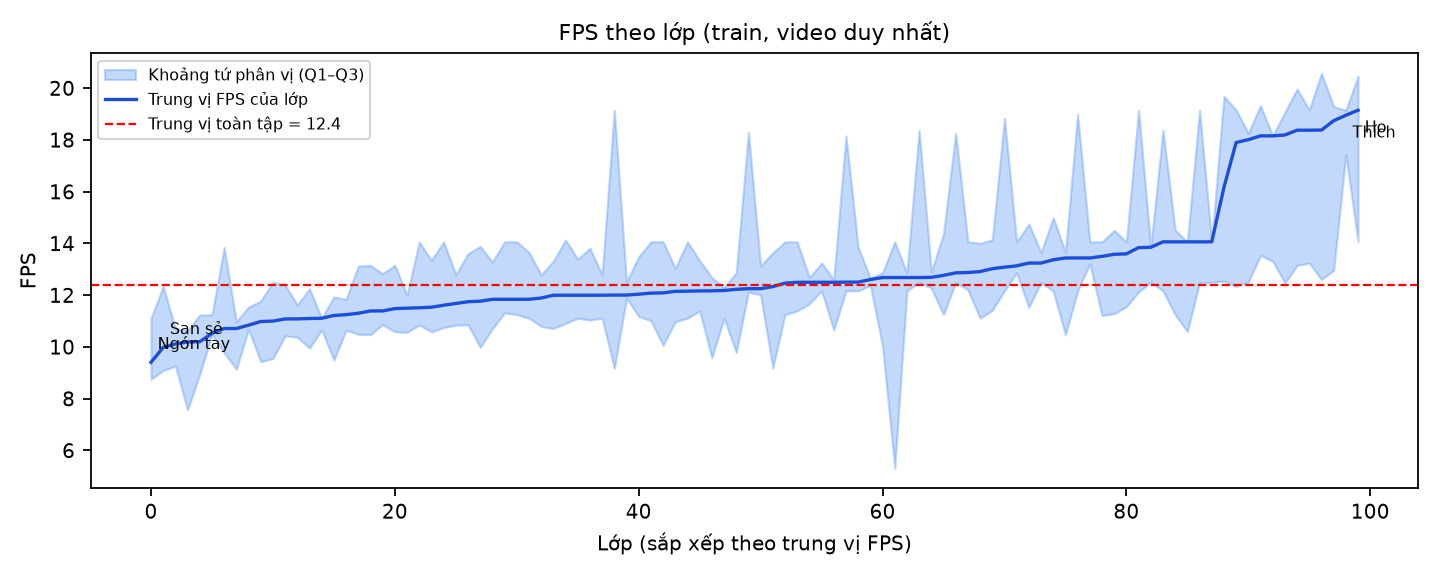
\includegraphics[width=0.95\textwidth]{fps_by_class.png}
  \caption{Trung vị và khoảng tứ phân vị của FPS theo lớp (train, video duy nhất), các lớp sắp xếp theo trung vị.}
  \label{fig:eda_fps_class}
\end{figure}

\paragraph{Khung đơn sắc theo lớp} Khung đơn sắc không phân bố đều: 78/100 lớp có ít nhất một video bị ảnh hưởng, và có lớp có tới 30--40\% video duy nhất chứa khung đơn sắc (\textit{Có thể}, \textit{Xin lỗi}, \textit{Thất lạc}, \textit{Mua}). Do đó việc loại bỏ khung đơn sắc sẽ tác động không đồng đều lên các lớp.

\noindent\textit{Hệ quả:} (i) các thuộc tính metadata phần lớn độc lập nhau nên không có cặp đặc trưng dư thừa cần loại bỏ; (ii) vì FPS và dung lượng có quan hệ thống kê với nhãn, chúng có thể trở thành ``đường tắt'' (\textit{shortcut}) mà mô hình học được thay vì học ký hiệu, nên không nên đưa FPS hoặc dung lượng làm đặc trưng đầu vào và cần theo dõi nguy cơ này khi đánh giá; (iii) cần kiểm tra lại phân phối nhãn sau khi loại khung đơn sắc.

% =====================================================================
\subsubsection{So sánh phân phối giữa các tập}
\label{subsec:eda_shift}

\paragraph{Script và cách thực hiện}
\begin{itemize}
  \item \textbf{Script:} \edafile{06\_split\_comparison}{01\_split\_shift.py}.
  \item \textbf{Cách khai thác dữ liệu:} với train chỉ giữ video duy nhất, để các bản sao không làm lệch phân phối. Với mỗi thuộc tính (\texttt{frames}, \texttt{fps}, \texttt{dur}, \texttt{size\_kb}, \texttt{motion}), script tính trung vị từng tập và chạy kiểm định Kolmogorov--Smirnov hai mẫu (\texttt{scipy.stats.ks\_2samp}) cho từng cặp tập. Thống kê $D$ là khoảng cách lớn nhất giữa hai hàm phân phối tích luỹ thực nghiệm (ECDF); $D$ càng lớn thì hai phân phối càng khác nhau. Script cũng tính tỷ lệ video có khung đơn sắc ở từng tập và số video trùng nội dung giữa các tập (theo \texttt{file\_hashes.csv}). Ngưỡng ngoại lai trên của dung lượng (167~KB, tính từ train) lấy từ bước đơn biến.
  \item \textbf{Đầu ra:} \texttt{split\_shift\_summary.txt}, \texttt{ecdf\_by\_split.png}.
\end{itemize}

Nhóm so sánh phân phối các thuộc tính giữa ba tập trên cùng trục (Bảng~\ref{tab:eda_desc}, Bảng~\ref{tab:eda_ks}, Hình~\ref{fig:eda_ecdf}) để tìm dấu hiệu khác biệt miền (\textit{Domain Shift}).

\begin{table}[H]
  \centering
  \caption{Kiểm định Kolmogorov--Smirnov hai mẫu giữa các tập (train: video duy nhất). Giá trị là thống kê $D$, trong ngoặc là $p$-value.}
  \label{tab:eda_ks}
  \small
  \begin{tabular}{@{}lccc@{}}
    \toprule
    \textbf{Thuộc tính} & \textbf{train -- public} & \textbf{train -- private} & \textbf{public -- private} \\
    \midrule
    Số khung        & 0,005 (1)                 & 0,007 (1)                 & 0,002 (1) \\
    FPS             & 0,075 ($1{,}7\cdot10^{-5}$) & 0,069 ($2{,}9\cdot10^{-6}$) & 0,094 ($1{,}7\cdot10^{-8}$) \\
    Thời lượng      & 0,075 ($1{,}7\cdot10^{-5}$) & 0,068 ($4{,}5\cdot10^{-6}$) & 0,094 ($1{,}7\cdot10^{-8}$) \\
    Dung lượng      & \textbf{0,230} ($2\cdot10^{-48}$) & \textbf{0,237} ($4\cdot10^{-70}$) & 0,059 (0,0013) \\
    Chuyển động     & 0,059 (0,0015)            & 0,079 ($4{,}8\cdot10^{-8}$) & 0,035 (0,15) \\
    \bottomrule
  \end{tabular}
\end{table}

\begin{figure}[H]
  \centering
  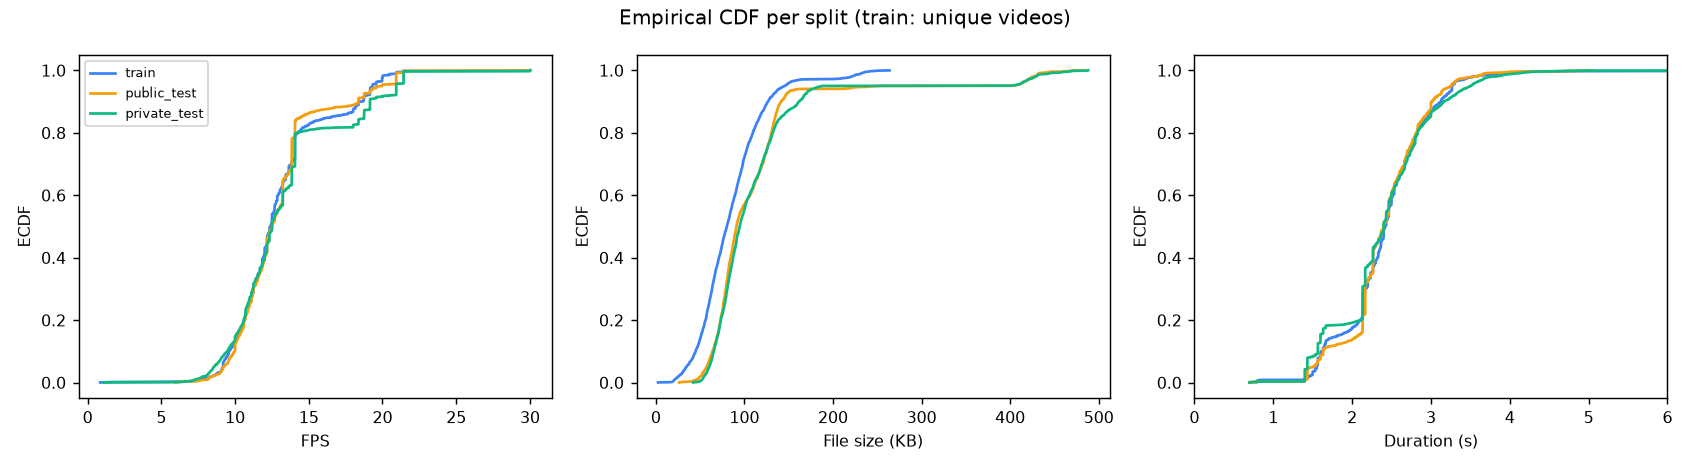
\includegraphics[width=\textwidth]{ecdf_by_split.png}
  \caption{Hàm phân phối tích luỹ thực nghiệm của FPS, dung lượng và thời lượng theo tập (train: video duy nhất). Đường dung lượng của train tách hẳn khỏi hai tập test.}
  \label{fig:eda_ecdf}
\end{figure}

Vì cỡ mẫu lớn nên mọi khác biệt dù nhỏ đều có $p$ rất bé; nhóm đánh giá chủ yếu theo độ lớn của $D$. Số khung hình giống nhau ở cả ba tập ($D<0{,}01$), độ phân giải cũng vậy. FPS, thời lượng và độ chuyển động khác biệt nhỏ ($D<0{,}1$). Riêng dung lượng khác biệt rõ giữa train và hai tập test ($D\approx0{,}23$--$0{,}24$), trong khi hai tập test gần nhau ($D\approx0{,}06$). Cụ thể:

\begin{itemize}
  \item \textbf{Dung lượng:} video test nặng hơn đáng kể (trung bình 113,6--116,3~KB so với 85,5~KB; trung vị 91,0--94,6~KB so với 80,6~KB). Tỷ lệ video vượt 167~KB (ngưỡng ngoại lai của train) là 3,1\% ở train nhưng 6,0\% ở public và 8,2\% ở private. Một phần chênh lệch có thể giải thích bởi khung đơn sắc (nén rất nhỏ) chỉ có ở train: trung vị dung lượng của video train có khung đơn sắc là 49,0~KB, còn của video train không có khung đơn sắc là 87,6~KB, gần mức của test. Tuy nhiên đuôi dài tới 488~KB ở test không xuất hiện ở train (lớn nhất 263,8~KB), cho thấy test có thể chứa các video chi tiết hoặc nhiễu hơn.
  \item \textbf{FPS:} trung vị gần như nhau (12,4 ở train, 12,5 ở hai tập test), nhưng private test có độ lệch chuẩn lớn hơn (3,69 so với 3,11 ở train) và đuôi dài hơn.
  \item \textbf{Khung đơn sắc:} khoảng 20\% video train nhưng gần như không có ở test (Bảng~\ref{tab:eda_solid}).
  \item \textbf{Người ký, nền, ánh sáng:} có thể khác giữa train và test; nhóm chưa định lượng được yếu tố này.
\end{itemize}

\noindent\textit{Hệ quả:} cần các phép tăng cường giúp mô hình bền vững với thay đổi màu sắc, độ sáng và khung cắt (\textit{ColorJitter}, \textit{Random Resized Crop}); việc loại bỏ khung đơn sắc ở train đồng thời giúp thu hẹp khoảng cách giữa phân phối train và test.

% =====================================================================
\subsubsection{Kết luận EDA và khuyến nghị cho bước tiền xử lý}
\label{subsec:eda_conclusion}

Bảng~\ref{tab:eda_reco} tổng hợp các vấn đề phát hiện được, bằng chứng và khuyến nghị cho bước tiền xử lý (Mục~\ref{sec:preprocess}) cũng như huấn luyện.

\begin{table}[H]
  \centering
  \caption{Tổng hợp vấn đề, bằng chứng và khuyến nghị cho bước tiền xử lý.}
  \label{tab:eda_reco}
  \small
  \begin{tabular}{@{}p{0.2\textwidth}p{0.36\textwidth}p{0.38\textwidth}@{}}
    \toprule
    \textbf{Vấn đề} & \textbf{Bằng chứng} & \textbf{Khuyến nghị} \\
    \midrule
    Tên lớp khác dạng Unicode & Khoá trong \texttt{label\_mapping.pkl} ở dạng NFD, thư mục lớp ở dạng NFC; 91/100 lớp không khớp nếu so nguyên văn & Chuẩn hoá NFC cả hai phía trước khi tra nhãn \\
    \addlinespace
    Video trùng lặp (\texttt{\_N}) & 1.069 tệp \texttt{\_N} giống hệt bản gốc; chỉ còn 2.776 video duy nhất & Khử trùng lặp theo MD5; chia train/validation theo ID gốc (bỏ hậu tố \texttt{\_N}) bằng \texttt{StratifiedGroupKFold} để tránh rò rỉ \\
    \addlinespace
    Mất cân bằng lớp & 6--74 video/lớp (sau khử trùng lặp: 5--51), 36/100 lớp có $\leq$25 video & Dùng Macro F1; trọng số lớp hoặc \texttt{WeightedRandomSampler}; oversample kèm tăng cường cho lớp ít mẫu; có thể dùng label smoothing \\
    \addlinespace
    Khung đơn sắc & 565/2.776 video duy nhất (20,4\%) chứa trung bình 12,2 khung đơn sắc; test gần như không có & Loại bỏ khung đơn sắc (độ lệch chuẩn điểm ảnh $<3$) \emph{trước} khi lấy mẫu $T=16$; nếu còn ít hơn 16 khung hợp lệ thì lặp khung \\
    \addlinespace
    Video rỗng & \texttt{Biết/214576}, \texttt{Khai báo/885339} (cùng 2 bản sao) đơn sắc toàn bộ & Loại khỏi tập huấn luyện \\
    \addlinespace
    Xung đột nhãn & 2 nhóm nội dung giống hệt nhưng thuộc \textit{Chậm lại} và \textit{Chào} & Xác minh nhãn đúng; nếu không xác minh được thì loại bỏ \\
    \addlinespace
    Độ dài không đồng nhất & 98,9\% video có 30 khung, tối thiểu 16 khung; thời lượng tới 35,3~s & Lấy mẫu $T=16$ khung đều bằng \texttt{linspace} \\
    \addlinespace
    FPS/dung lượng liên hệ với nhãn & $\eta^2\approx0{,}28$ (FPS), $0{,}15$ (dung lượng) giữa các lớp & Không dùng FPS, dung lượng làm đặc trưng; theo dõi nguy cơ shortcut \\
    \addlinespace
    Khác biệt miền train--test & Test nặng hơn (trung bình 114--116~KB so với 85,5~KB; KS $D\approx0{,}23$); khung đơn sắc chỉ có ở train & ColorJitter, Random Resized Crop, chuẩn hoá ImageNet; \emph{không} lật ngang \\
    \addlinespace
    Trùng train--public test & 157 video public giống hệt video train & Lưu ý khi diễn giải điểm public test \\
    \bottomrule
  \end{tabular}
\end{table}

Tóm lại, bộ dữ liệu có định dạng rất đồng nhất (100\% video $224\times224$, gần như đều 30 khung), nên khâu đọc và lấy mẫu khung đơn giản. Tuy nhiên dữ liệu huấn luyện có ba vấn đề cần xử lý trước khi huấn luyện: mất cân bằng lớp, khoảng 28\% tệp là bản sao gây nguy cơ rò rỉ dữ liệu, và khoảng 20\% video chứa khung đơn sắc vốn không xuất hiện ở dữ liệu kiểm tra. Đây là những yếu tố có thể khiến điểm validation cao hơn đáng kể so với điểm thực tế trên tập kiểm tra nếu không được xử lý.

\paragraph{Hạn chế của phân tích} FPS và thời lượng đọc từ metadata của container nên có thể không phản ánh tốc độ quay thực. Ngưỡng độ lệch chuẩn $<3$ chỉ phát hiện khung đơn sắc hoàn toàn, chưa phát hiện khung mờ hoặc chỉ có nền. Nhóm chưa định lượng sự khác biệt về người ký và bối cảnh giữa train và test, chưa xác định được nguyên nhân FPS liên hệ với nhãn, và chưa xác định được nhãn đúng cho các video xung đột.
